% !TeX program = pdflatex
\documentclass{iutbscthesis}

% ---------------------------------------------------------------------
% Extra packages used by this thesis, beyond what iutbscthesis.cls loads
% ---------------------------------------------------------------------
\usepackage{multirow}     % merged cells in wide result tables
\usepackage{longtable}    % appendix tables that span multiple pages
\usepackage{tikz}         % pipeline / architecture diagrams
\usetikzlibrary{arrows.meta, positioning, fit, backgrounds}

% The iutbscthesis class already provides \addbibresource via biblatex.
\addbibresource{citations.bib}

% =======================================================================
% FRONT-MATTER METADATA
% Everything in this block that says "PLACEHOLDER" is administrative
% information only the candidate(s) and the department can supply.
% Replace it before printing/submission; nothing else in this file
% needs to change to accommodate that.
% =======================================================================

\title{Reliability in Few-Shot Classification with Frozen CNN Adapters: A Controlled Study}

\addauthor{Hamim Saad Al Raji}{210042143}
\addauthor{MD Mainul Hasan}{210042173}
\addauthor{Ahmed Sadman Labib}{210042135}

\supervisor{Shahriar Ivan}{Assistant Professor}{Department of Computer Science and Engineering}

% No co-supervisor for now. If one is confirmed later, uncomment and fill in:
% \addcosupervisor{Md.\ Bakhtiar Hasan}{Assistant Professor}{Department of Computer Science and Engineering}

\department{Department of Computer Science and Engineering}
\program{BACHELOR OF SCIENCE IN COMPUTER SCIENCE AND ENGINEERING}

\defensedate{17}{September}{2026}

\begin{document}
\hfuzz=0.1pt
\hbadness=0

%-------------------------- FRONT MATTER --------------------------%

\coverpage

\pagenumbering{roman}

\titlepage

\declarationofcandidate

\dedicatedto{everyone who insisted that a model's confidence should mean something}

\tableofcontents
\listoffigures
\listoftables

\clearpage

\begin{abbreviations}
    \abbr{AUROC}{Area Under the Receiver Operating Characteristic Curve}
    \abbr{BSc}{Bachelor of Science}
    \abbr{CNN}{Convolutional Neural Network}
    \abbr{ECE}{Expected Calibration Error}
    \abbr{EDL}{Evidential Deep Learning}
    \abbr{FPR}{False Positive Rate}
    \abbr{FPR@95}{False Positive Rate at 95\% True Positive Rate}
    \abbr{FLOPs}{Floating-Point Operations}
    \abbr{ID}{In-Distribution}
    \abbr{KL}{Kullback--Leibler (divergence)}
    \abbr{LoRA}{Low-Rank Adaptation}
    \abbr{MCU}{Microcontroller Unit}
    \abbr{MSP}{Maximum Softmax Probability}
    \abbr{OOD}{Out-of-Distribution}
    \abbr{PEFT}{Parameter-Efficient Fine-Tuning}
    \abbr{ProtoNet}{Prototypical Network}
    \abbr{ResNet}{Residual Network}
    \abbr{TPR}{True Positive Rate}
    \abbr{TS}{Temperature Scaling}
    \abbr{ViT}{Vision Transformer}
    \abbr{W\&B}{Weights \& Biases (experiment tracking tool)}
    \abbr{YAML}{YAML Ain't Markup Language}
\end{abbreviations}

\begin{acknowledgement}

We are sincerely grateful to our supervisor, \textbf{Shahriar Ivan}, Assistant Professor, Department of Computer Science and Engineering, for the guidance, patience, and critical feedback that shaped this thesis from an initial one-episode proof of concept into a full experimental study spanning fourteen development steps. His willingness to let a negative result stand as a negative result, rather than pushing us to paper over it, is the reason this thesis can honestly report what it found rather than what it hoped to find.

We thank the Department of Computer Science and Engineering, Islamic University of Technology, for the environment, coursework, and computing support that made this research possible, and the faculty members whose courses in machine learning and probability directly underpin the Bayesian and evidential formulations used here.

This work relied heavily on freely available cloud compute: Google Colab and Kaggle's Tesla T4 GPU instances carried essentially all 120 grid runs, the 48-run matched-budget experiment, and the efficiency benchmarking reported in this thesis, at zero cost to the department. We are grateful to the maintainers of PyTorch, Weights \& Biases, and the broader open-source scientific Python ecosystem, without which a project of this experimental scale would not have been tractable for a bachelor's thesis timeline.

Finally, we thank our families and friends for their patience during the months in which a laptop screen full of ECE numbers seemed, to us, like the most interesting thing in the world.

\end{acknowledgement}

\begin{abstract}
Parameter-efficient fine-tuning (PEFT) lets a large pretrained network adapt to a new task by training only a small fraction of its parameters, but almost all PEFT research targets Vision Transformers evaluated on data-rich benchmarks, leaving open how PEFT behaves inside convolutional architectures under the two constraints that matter for edge deployment: severe data scarcity (few-shot learning) and the requirement that reported confidence be trustworthy. This thesis studies B-PEFT, a framework for reliable few-shot vision with lightweight, frozen CNN backbones (ResNet-18 and MobileNetV3-Small). A single trainable adapter — bottleneck, LoRA, or BitFit, with full fine-tuning and linear probing as baselines — is inserted into an otherwise frozen, ImageNet-pretrained backbone, and classification is performed by a parameter-free prototype head whose similarity logits are read either as ordinary softmax probabilities or, following Evidential Deep Learning, as evidence for a Dirichlet distribution over class probabilities, yielding a principled epistemic-uncertainty score (vacuity) at negligible extra inference cost. The system is evaluated on 5-way $k$-shot episodes from CIFAR-FS and MiniImageNet against far- and near-out-of-distribution pools (SVHN, Gaussian noise, CIFAR-100-heldout, TinyImageNet), measuring accuracy, calibration (Expected Calibration Error, Brier score), and out-of-distribution detection (AUROC, FPR at 95\% true-positive rate) over a balanced 120-run grid crossing dataset, shot count, backbone, adapter, and head interpretation. Four initial, comparison-framed research questions — does parallel adapter placement beat serial placement; does an evidential head calibrate better than softmax under a tiny parameter budget; does the evidential objective improve near-out-of-distribution detection; and what is the latency-versus-uncertainty-quality trade-off — were each answered on the grid, but a literature audit found three of the four substantially anticipated by prior work. This motivated a second, attribution-framed set of questions asked over the same data: how outcome variance is distributed across the experimental design axes; whether the observed uncertainty benefit is produced by the training objective or by the post-hoc scoring rule; whether adapter architecture or trainable-parameter budget governs accuracy and calibration; and whether the evidential head's calibration deficit can be remediated after training without destroying its ranking quality. A pre-registered, matched-parameter-budget follow-up experiment resolves the hardest of these: accuracy and near-out-of-distribution detection track adapter architecture regardless of which adapter holds the larger parameter budget, while the calibration gap between adapters is intrinsic to the backbone rather than to the budget. The evidential head is shown to be a substantially better out-of-distribution ranker than softmax-probability-based scores, though a training-free energy score still ranks better than it in most configurations, and its calibration deficit can be reduced by two orders of magnitude fewer parameters than the adapter itself uses — refitting only two evidence-affine parameters on a held-out split — while preserving its ranking quality in the large majority of cases.
\end{abstract}

%-------------------------- MAIN BODY --------------------------%
\pagenumbering{arabic}

% =======================================================================
\chapter{Introduction}
\label{chapter:introduction}
% =======================================================================

This thesis is a controlled study of which design choices govern which aspects of reliability in a parameter-efficient, few-shot vision system. No single design choice makes a few-shot model reliable on every axis at once; \autoref{tab:opening-summary} previews the headline mapping this thesis establishes, elaborated and evidenced fully in \autoref{chapter:results} and restated with supporting evidence in \autoref{tab:conclusion-summary}.

\begin{table}[H]
    \centering
    \small
    \begin{tabular}{l >{\raggedright\arraybackslash}p{9.5cm}}
        \toprule
        Reliability aspect & Governed mainly by \\
        \midrule
        Accuracy & shot count + adapter architecture \\
        Calibration & head type + backbone \\
        OOD detection & the uncertainty scoring rule \\
        Calibration repair & a post-hoc refit: it improves calibration but does not fully fix it \\
        \bottomrule
    \end{tabular}
    \caption{No single design choice makes a few-shot model reliable on every axis.}
    \label{tab:opening-summary}
\end{table}

\section{Background and Motivation}

Deep convolutional networks pretrained on large image corpora such as ImageNet~\cite{deng2009imagenet} learn feature representations that transfer well to new visual tasks. The dominant way to reuse such a network is fine-tuning: continuing gradient descent on all of its parameters using data from the new task. Fine-tuning a modern backbone end to end, however, means updating millions of parameters, which is wasteful when the downstream task provides only a handful of labelled examples, and risky, because a model with millions of degrees of freedom and tens of images to learn from will overfit almost by construction. This is precisely the regime of \emph{few-shot learning}: given only $k$ labelled examples per class (typically $k \in \{1, 5\}$), the model must classify unseen images correctly on classes it has never encountered in training.

Parameter-Efficient Fine-Tuning (PEFT) responds to this problem by freezing the pretrained backbone entirely and inserting a small number of trainable parameters — an \emph{adapter} — that reshapes the backbone's features for the new task. Adapters of this kind, first popularised for natural-language transformers by \textcite{houlsby2019adapters} and later refined into low-rank (\textcite{hu2022lora}) and bias-only (\textcite{benzaken2022bitfit}) variants, can match or approach full fine-tuning accuracy while training a fraction of a percent of the backbone's parameters. Almost all of this literature, however, was built for and evaluated on Vision Transformers on data-rich benchmarks; how the same idea behaves inside a \emph{convolutional} architecture, under \emph{few-shot} data scarcity, is comparatively unexplored — despite convolutional networks remaining the practical choice for any deployment target too small, too power-constrained, or too latency-sensitive to run a transformer, which describes essentially all microcontroller-class edge hardware~\cite{somvanshi2025tinydl}.

A second, largely separate problem is reliability. A classifier is not merely asked to be accurate; in any setting where its output informs a downstream decision — a medical triage suggestion, an autonomous system's fallback trigger — the classifier's stated confidence needs to mean something. A model that reports ``95\% confident'' while being correct only 60\% of the time is \emph{miscalibrated}, and \textcite{guo2017calibration} showed that modern, high-capacity neural networks are miscalibrated by default, becoming more confident as they become more accurate rather than more honest. A closely related but distinct requirement is out-of-distribution (OOD) detection: the ability to recognise that an input does not belong to any of the classes the model was trained to distinguish, and to say so via a low-confidence or high-uncertainty output rather than a confident wrong answer~\cite{hendrycks2017baseline}. Standard softmax classifiers are known to produce overconfident, poorly separated outputs for exactly this case. Evidential Deep Learning (EDL), introduced by \textcite{sensoy2018edl}, offers an alternative: rather than outputting a single point estimate of class probabilities, the network outputs the parameters of a Dirichlet distribution \emph{over} class probabilities, from which both a prediction and a principled measure of epistemic uncertainty (how much evidence the network has actually seen, as opposed to how sharply it happens to be guessing) can be read off in a single deterministic forward pass — no sampling, no ensembling, no Monte Carlo dropout.

This thesis sits at the intersection of these three lines of work — parameter-efficient adaptation, convolutional (rather than transformer) backbones, and evidential uncertainty — under the added constraint of few-shot data scarcity, and asks a question none of the individual literatures answer on its own: \emph{when a lightweight CNN is adapted to a new task using only a handful of examples and a few thousand trainable parameters, does an evidential uncertainty mechanism actually deliver more trustworthy predictions than the softmax baseline, and at what cost?}

\section{Problem Statement}

Three specific problems motivate the design of this thesis, all stemming from one observation: \textbf{a model can be accurate and still unreliable.} \autoref{fig:accuracy-vs-reliability} illustrates the two ways this happens. A model can be accurate overall while being confidently \emph{wrong} on a specific known-class input (miscalibration — its stated confidence does not track its actual correctness), and it can be accurate on the classes it recognises while producing an equally confident answer for an input from a class it was never designed to recognise at all (no OOD flag). Neither failure shows up in a top-1 accuracy number, which is exactly why this thesis measures calibration and out-of-distribution detection alongside accuracy throughout.

\begin{figure}[H]
    \centering
    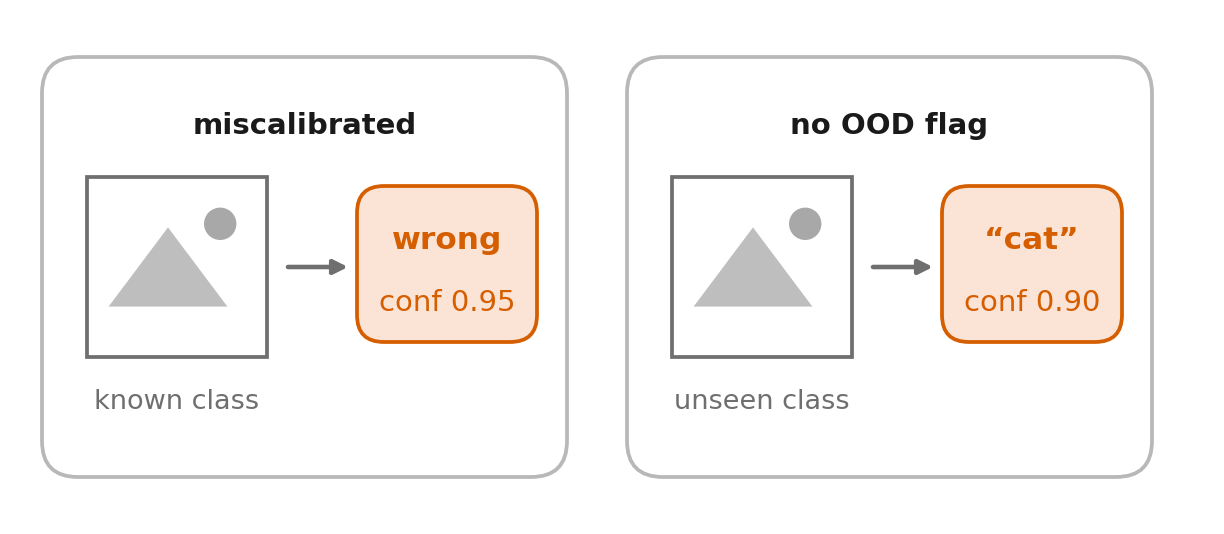
\includegraphics[width=0.75\textwidth]{figures/D1_accuracy_vs_reliability.png}
    \caption{Accuracy is not reliability. Left: a known-class input, confidently misclassified (miscalibration). Right: an input from an unseen class, confidently assigned to a known class with no indication of uncertainty (no OOD flag).}
    \label{fig:accuracy-vs-reliability}
\end{figure}

\paragraph{Parameter inefficiency.} Full fine-tuning of a CNN on a small few-shot dataset causes catastrophic forgetting of the pretrained representation and severe overfitting: with only one to five images per class, a model with millions of trainable parameters has essentially no statistical basis for its updates. A parameter-efficient alternative must be found that adapts the backbone's features without retraining the backbone itself.

\paragraph{The reliability gap.} Standard PEFT methods inherit whatever confidence behaviour the base model exhibits, and typically report only accuracy. A PEFT method that reaches high accuracy while remaining silently overconfident, or unable to flag inputs from classes it was never designed to recognise, is not safe to deploy in any setting where a wrong-but-confident answer is more costly than an honest ``I don't know.''

\paragraph{Architectural bias in the PEFT literature.} The great majority of PEFT research — adapters, LoRA, visual prompt tuning, and their many descendants — targets Vision Transformers~\cite{jia2022vpt, chen2022adaptformer, jie2023fact, zhang2022noah, lian2022ssf}. CNNs have different structural properties from transformers: locality, translation invariance, and a hierarchical (rather than globally attentive) feature extraction process. How an adapter interacts with a convolutional block — where it should be placed, and what form it should take — is not well understood, and the handful of works that do study CNN-side PEFT (\textcite{chen2024convadapter}; \textcite{aleem2024convlora}; \textcite{zhong2024convlorasam}) rarely combine it with an uncertainty-aware training objective or a rigorous OOD evaluation.

\autoref{tab:problem-response} summarises the three problems above against this thesis's response to each, stated as the concrete design decision that addresses it.

\begin{table}[H]
    \centering
    \small
    \begin{tabular}{>{\raggedright\arraybackslash}p{5.5cm} >{\raggedright\arraybackslash}p{7cm}}
        \toprule
        Challenge & This thesis's response \\
        \midrule
        Full fine-tuning updates millions of weights & Freeze the backbone; train at most 31.7K adapter parameters once. New classes require no further gradient-based adaptation. \\
        PEFT studies rarely measure reliability & Measure accuracy, calibration, \emph{and} OOD detection on the same runs. \\
        PEFT research focuses on transformers & Study adapters inside lightweight, frozen CNNs. \\
        \bottomrule
    \end{tabular}
    \caption{The three challenges motivating this thesis, and its response to each.}
    \label{tab:problem-response}
\end{table}

\section{Research Questions}
\label{sec:intro-rqs}

The project's initial research proposal posed four comparison-style questions, each of the form ``does approach A outperform approach B'' (adapter placement, evidential-versus-softmax calibration, Bayesian near-OOD detection, and a latency/uncertainty Pareto frontier). Before those answers were written up as contributions, a systematic literature check was carried out against each one, and found that three of the four had close, sometimes near-identical, precedent in prior work: the placement question is answered in essentially the same direction, on the same frozen ResNet-18 backbone and protocol, by \textcite{li2022tsa}; the near-OOD claim is the standard, well-established evidential-learning result once the comparison is restricted to softmax-probability baselines; and the Pareto-frontier reporting style is a presentational device rather than a novel finding. This motivated reframing the underlying experimental grid — the same 120 completed runs, the same metrics, the same datasets — around four \emph{attribution}-style questions, which ask not which of two options is better but \emph{what governs the outcome} across the full space of design choices. No experiment from the original four questions is discarded; each is folded into the discussion of whichever of the four questions below it now serves as evidence for (\autoref{sec:results-positioning} and \autoref{chapter:results} note explicitly where this happens). These four questions are what \autoref{chapter:results} is built around, and they are the thesis's primary scientific contribution:

\begin{description}
    \item[RQ1.] Which design choices most strongly explain variation in accuracy, calibration, and out-of-distribution detection? More precisely: how is variance in each outcome distributed across the principal design axes of a parameter-efficient few-shot classification system — dataset, shot count, backbone, adapter type, and uncertainty-head interpretation?
    \item[RQ2.] Is out-of-distribution detection explained more by the training objective, or by the scoring rule? More precisely: is OOD-detection performance attributable to the training objective under which the model was adapted (evidential versus softmax), or to the post-hoc scoring rule by which its outputs are read (vacuity, maximum softmax probability, or energy) — and can the two be separated experimentally?
    \item[RQ3.] Does accuracy follow adapter architecture, and calibration follow parameter budget? More precisely: within the adapter axis, are accuracy and calibration governed by the same property of an adapter, or does accuracy follow the adapter's \emph{architecture} while calibration follows its trainable-\emph{parameter budget} — or something else entirely?
    \item[RQ4.] Can evidential calibration be repaired after training, without breaking out-of-distribution detection? More precisely: can the calibration of an evidential prototype head be improved after training, by refitting only the two parameters of its evidence-affine transform on held-out validation episodes, without destroying the head's OOD ranking ability?
\end{description}

\autoref{tab:rq-roadmap} summarises what each question is answered by, and \autoref{fig:research-roadmap} shows how all four sit under one overarching question.

\begin{table}[H]
    \centering
    \small
    \begin{tabular}{l >{\raggedright\arraybackslash}p{7.5cm} >{\raggedright\arraybackslash}p{4cm}}
        \toprule
        & Question & Answered by \\
        \midrule
        RQ1 & Which design choices most strongly explain variation in accuracy, calibration and OOD detection? & 120-run factorial grid \\
        RQ2 & Is OOD detection explained more by the training objective or by the scoring rule? & All 120 models re-scored with 4 scores \\
        RQ3 & Does accuracy follow adapter architecture, and calibration follow parameter budget? & Grid + matched-budget experiment \\
        RQ4 & Can evidential calibration be repaired after training without breaking OOD detection? & Post-hoc refit of 60 evidential models \\
        \bottomrule
    \end{tabular}
    \caption{The four research questions and the evidence each is answered by.}
    \label{tab:rq-roadmap}
\end{table}

\begin{figure}[H]
    \centering
    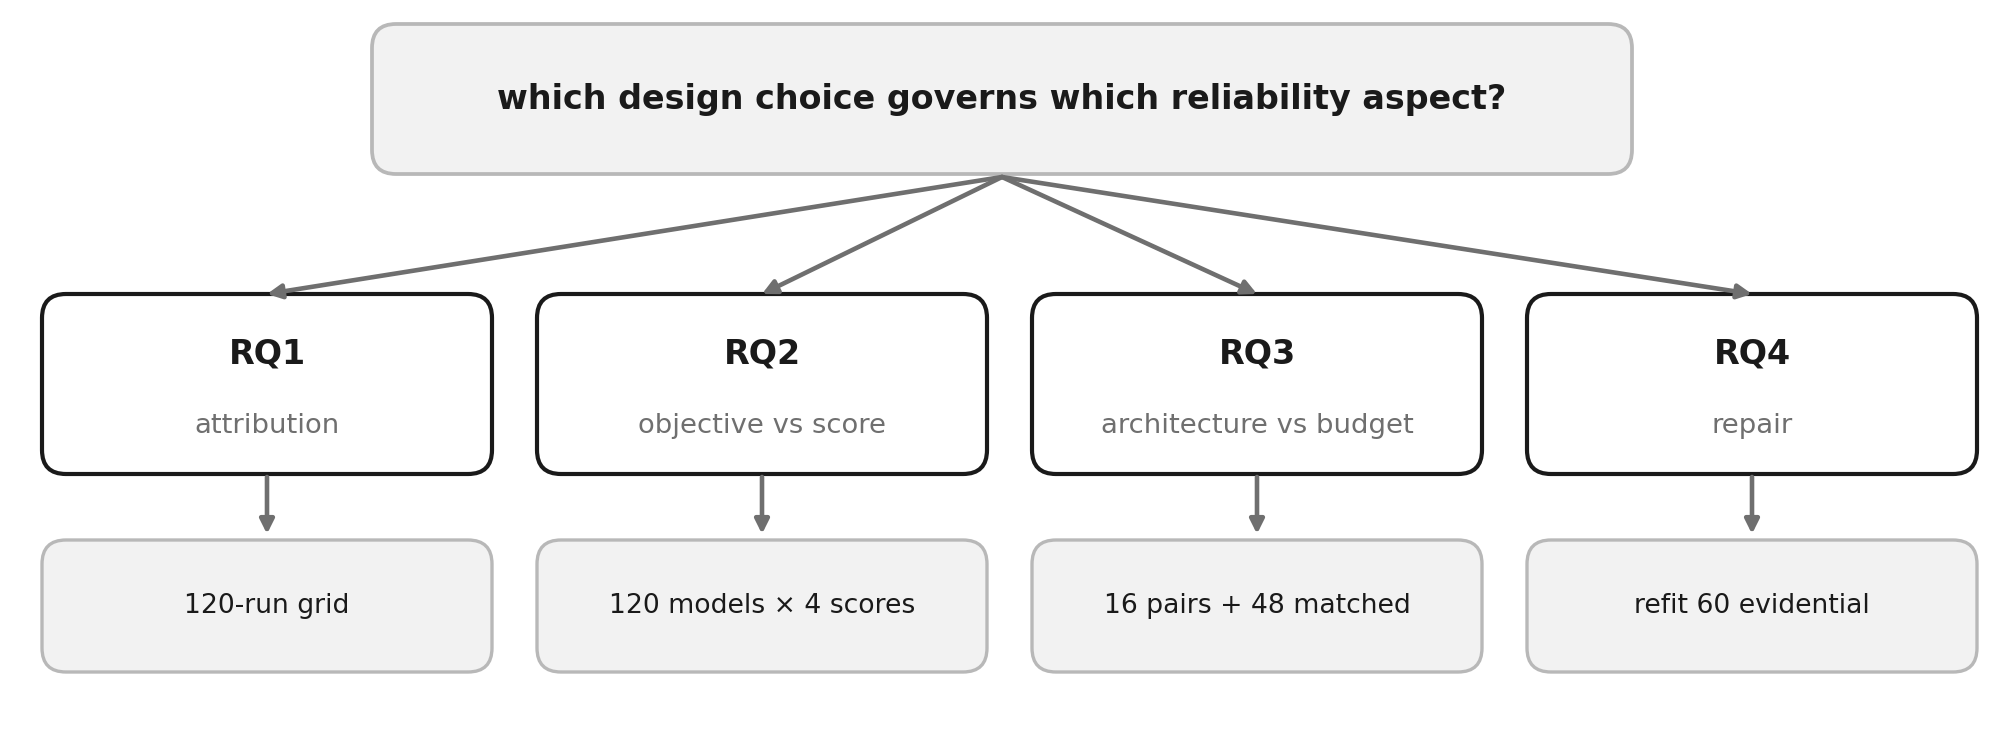
\includegraphics[width=0.95\textwidth]{figures/F1_research_roadmap.png}
    \caption{All four research questions are instances of one overarching question — which design choice governs which reliability aspect — each resolved by a specific, named piece of evidence.}
    \label{fig:research-roadmap}
\end{figure}

\section{Research Challenges}

Several challenges specific to this problem domain shaped the design of the study.

\paragraph{Confounded comparisons.} A naive comparison between two adapter types, or two backbones, is rarely a comparison of one property at a time: a larger adapter is usually also a different \emph{kind} of adapter, and a more accurate backbone is usually also a larger one. Disentangling architecture from parameter budget — the central concern of RQ3 — required first identifying a structural coincidence in the grid (the parameter-budget ordering of two adapters reverses between the two backbones used) and then, because that coincidence alone could not fully separate the two explanations, designing and running a dedicated matched-budget experiment (\autoref{sec:results-matched-budget}).

\paragraph{The evidential-collapse failure mode.} Early in development, a specific and easy-to-miss numerical failure occurred: the raw similarity logits produced by the parameter-free prototype head are large and negative, so passing them directly through the evidential mapping's non-linearity collapsed all evidence to zero, producing a uniform Dirichlet distribution and dead training gradients regardless of the input. This is exactly the kind of failure the project's governing implementation guidance warns to watch for — a technique that fails silently under conditions the original paper never tested — and its fix (an affine rescaling of the logits before the non-linearity, \autoref{sec:method-evidence-affine}) became a load-bearing design decision rather than an incidental implementation detail.

\paragraph{Reproducibility under a small-sample, high-variance regime.} Few-shot accuracy is measured over episodes sampled from a small pool of classes, so a single training run's result can be an artefact of which classes happened to be sampled for evaluation rather than a property of the method. The response taken throughout this thesis is to freeze a single set of 600 test-episode seeds for every evaluation (\autoref{sec:proto-episodic}) and to report results across three independent training seeds, rather than reporting a single number per configuration.

\paragraph{An honest audit trail.} Because several of the thesis's headline claims evolved under scrutiny — an early single-configuration result suggesting evidential uncertainty was competitive with the energy score did not survive a full 120-run grid (\autoref{sec:results-rq2}); an apparent interior optimum in calibration versus parameter budget did not survive a controlled rank sweep (\autoref{sec:results-rq5-demoted}) — this thesis reports corrected findings alongside the reasoning that produced the correction, rather than presenting only the final, cleaned-up narrative.

\section{Contributions}

This thesis makes the following contributions:

\begin{enumerate}
    \item A working B-PEFT system — a frozen, ImageNet-pretrained lightweight CNN backbone (ResNet-18 or MobileNetV3-Small), a choice of parameter-efficient adapter (bottleneck, LoRA, or BitFit, with full fine-tuning and linear probing as non-PEFT baselines), and a parameter-free prototype head whose output can be read as either softmax probabilities or Dirichlet evidential uncertainty — implemented as a reproducible, config-driven codebase with deterministic seeding and byte-identical re-evaluation.
    \item A balanced, 120-run experimental grid (40 configurations $\times$ 3 seeds) crossing two datasets, two shot regimes, two backbones, two adapters, and two head interpretations, evaluated for accuracy, macro-F1, two calibration metrics, and OOD AUROC/FPR@95 against five OOD pools — to our knowledge the first factorial design of this breadth applied to a parameter-efficient, few-shot, uncertainty-aware CNN system, permitting a formal variance decomposition (RQ1) that most PEFT studies, which vary one axis at a time, cannot compute.
    \item A resolution of the confound between adapter \emph{architecture} and adapter \emph{parameter budget} in determining accuracy and calibration (RQ3), via a pre-registered, 48-run matched-budget experiment that equalises the two adapters' trainable-parameter counts within each backbone — closing an identification gap the base grid could not close on its own, and producing the corrected finding that accuracy and near-OOD detection follow adapter architecture while the calibration gap is intrinsic to the backbone rather than the parameter budget.
    \item A cross-factorial separation (RQ2) of the training objective (evidential versus softmax) from the OOD scoring rule (vacuity, maximum softmax probability, temperature-scaled maximum softmax probability, or energy) applied to it, showing that the scoring rule — not the training objective — accounts for roughly two to three orders of magnitude more OOD-detection variance on far-OOD pools (42.69\% versus 0.17\% $\eta^2$), a confound present, by the evaluated design's own admission, in the original grid and in closely related recent work.
    \item A demonstration (RQ4) that the evidential head's calibration deficit, established across the grid, can be substantially reduced by refitting only two parameters on a held-out validation split, at a cost several orders of magnitude smaller than the adapter itself, while measuring — rather than assuming — the extent to which the head's OOD ranking survives that refitting.
    \item An honest correction record: three findings from earlier stages of the project (an early evidential-versus-energy parity claim, an apparent interior-optimum in calibration-versus-budget, and a mis-scoped external citation) are explicitly superseded in this thesis by later, more rigorous experiments, with the superseded claims and the evidence that overturned them both reported.
\end{enumerate}

\section{Thesis Organization}

\autoref{chapter:related-works} surveys the five bodies of literature this thesis draws on — parameter-efficient fine-tuning, evidential and Bayesian deep learning, calibration, out-of-distribution detection, and few-shot learning — and positions this thesis's closest prior work. \autoref{chapter:background} defines the datasets, backbones, episodic protocol, and evaluation metrics used throughout. \autoref{chapter:methodology} describes the B-PEFT system itself: the adapters, the prototype head and its two interpretations, the evidential training objective, the post-hoc recalibration mechanism, and the design of the experimental grid and the matched-budget follow-up. \autoref{chapter:results} presents and interprets all results, first for the four original research questions and then for the four attribution questions that supersede them as the thesis's primary contribution, and closes with the system's positioning against comparable published work and a statement of the study's limitations. \autoref{chapter:conclusion} restates the research questions against what was found, summarises the contributions, and proposes concrete future work. \autoref{apx:results} reproduces the full 40-configuration result tables referenced selectively in \autoref{chapter:results}, and \autoref{apx:repro} documents the configuration and reproducibility conventions used to produce them.


% =======================================================================
\chapter{Related Works}
\label{chapter:related-works}
% =======================================================================

This thesis combines five bodies of work that are usually studied separately: parameter-efficient fine-tuning, Bayesian and evidential deep learning, calibration of neural network confidence, out-of-distribution detection, and few-shot learning. Each is surveyed in turn below, organised around the specific design decision it informs rather than as an annotated list, before \autoref{sec:related-positioning} positions this thesis directly against the handful of papers close enough to require explicit differentiation.

\section{Parameter-Efficient Fine-Tuning}
\label{sec:related-peft}

The founding idea of adapter-based PEFT, due to \textcite{houlsby2019adapters}, is to freeze a pretrained transformer and insert small bottleneck modules — a down-projection to a low-dimensional space, a non-linearity, and an up-projection back — between its layers, training only the bottlenecks. \textcite{hu2022lora} propose an alternative parameterisation, Low-Rank Adaptation (LoRA), which does not insert new modules but instead represents the \emph{update} to an existing weight matrix as the product of two low-rank matrices, $W_{\text{new}} = W_{\text{frozen}} + AB$ with $A \in \mathbb{R}^{d_{\text{out}} \times r}$ and $B \in \mathbb{R}^{r \times d_{\text{in}}}$ for a small rank $r$; because the update can be algebraically merged into $W_{\text{frozen}}$ after training, LoRA adds no inference-time latency, unlike a bottleneck module inserted in series. \textcite{benzaken2022bitfit} take efficiency further still, showing that training \emph{only} the bias terms of a transformer — under 0.1\% of its parameters — recovers a surprising fraction of full fine-tuning's accuracy on several NLP tasks. \textcite{he2022unified} unify this design space, showing that adapters, LoRA, and several other PEFT mechanisms can all be read as instances of one general update equation that differs only in where the update is inserted (\emph{serial}, after a sublayer, or \emph{parallel}, alongside it) and how it is parameterised — a vocabulary this thesis adopts directly for its own placement pilot (\autoref{sec:method-adapters}).

All of the above work targets transformer architectures. The convolutional case is thinner and more recent. \textcite{chen2024convadapter} study PEFT for CNNs directly and identify a specific failure mode relevant to adapter design inside convolutional blocks: an adapter implemented as a $1{\times}1$ (or fully-connected-style) transformation loses the \emph{spatial locality} that gives a CNN its inductive bias, whereas an adapter that preserves a local receptive field does not. This caveat directly informs how this thesis's own bottleneck and LoRA adapters are placed (\autoref{sec:method-adapters}). \textcite{aleem2024convlora} and \textcite{zhong2024convlorasam} independently develop convolutional forms of LoRA — applying the low-rank decomposition to convolutional kernels rather than fully-connected weight matrices — and report that this conv-form LoRA remains effective in low-data regimes, which this thesis's own LoRA implementation follows.

\section{Bayesian and Evidential Deep Learning}
\label{sec:related-edl}

Two largely separate traditions address the shortcomings of a point-estimate softmax classifier under uncertainty. The Bayesian tradition places a distribution over the network's \emph{weights} and marginalises over it at inference time, either exactly (intractable for any modern network), via ensembling~\cite{lakshminarayanan2017ensembles}, or via a tractable approximation. Evidential Deep Learning, introduced by \textcite{sensoy2018edl} and adopted as this thesis's mechanism, instead places a distribution over the network's \emph{output} — treating the classifier's final layer as producing \emph{evidence} $e_k \geq 0$ for each class $k$, interpreted as the parameters $\alpha_k = e_k + 1$ of a Dirichlet distribution over the categorical class-probability vector. The predictive probability for class $k$ is the Dirichlet mean $\hat p_k = \alpha_k / S$ where $S = \sum_k \alpha_k$ is the total Dirichlet strength, and the model's epistemic uncertainty (vacuity) is $u = K/S$ for $K$ classes: a network that has seen little relevant evidence for any class produces low $S$ and therefore high vacuity, regardless of how the available evidence is distributed among classes. Critically for a parameter-efficient setting, this uncertainty is available from a single deterministic forward pass, unlike ensembling or Monte Carlo dropout, which require multiple forward passes at inference time — a property \textcite{sensoy2018edl} present as EDL's central practical advantage and this thesis measures directly for its own system (\autoref{sec:results-implications}).

A body of recent work applies Bayesian machinery specifically to PEFT rather than to full networks. \textcite{yang2024laplacelora} (``Laplace-LoRA'') fit a post-hoc Laplace approximation over a trained LoRA module's parameters, substantially improving calibration on language-model benchmarks at low computational overhead; \textcite{wang2024blob} (``BLoB'') instead learn a variational Bayesian posterior over LoRA parameters during training. A wider landscape of similar Bayesian-LoRA variants — variational subspace inference~\cite{samplawski2025scalabl}, Stiefel-manifold priors~\cite{shihab2026stiefelbayes}, adaptive rank allocation~\cite{duan2026bara}, sparse Bayesian posteriors~\cite{zhang2026bayesiansparselora}, and even a dedicated benchmark for the sub-field~\cite{samplawski2026bagym} — has emerged in the last two years, but every one of these works targets \emph{large language models}; none evaluates a frozen \emph{vision} backbone, and none addresses the few-shot regime. A separately-named ``Bayesian-PEFT'' work~\cite{pandey2024bayesianpeft} is close enough in name to warrant an explicit note: it studies ViT foundation models with a base-rate-adjustment and evidential-ensembling mechanism, and does not address the architecture-versus-budget question this thesis's RQ3 resolves. \textcite{gao2024edlsurvey} survey the evidential-learning literature broadly and document the design rationale for the KL-divergence regulariser used in this thesis's own evidential loss (\autoref{sec:method-evidential-loss}).

The evidential mechanism is not without documented caveats. \textcite{bengs2022pitfalls} show that na\"ive loss-minimisation-based epistemic uncertainty estimators, including standard EDL objectives, can retain non-vanishing epistemic uncertainty even in the limit of infinite training data — a theoretical result consistent with, rather than contradicted by, this thesis's own empirical finding that the evidential head remains poorly calibrated across its entire tested parameter-budget range (\autoref{sec:results-rq1}). \textcite{shen2024mirage} more pointedly ask whether EDL's uncertainty quantification is real or a ``mirage,'' a question this thesis's own RQ2 (\autoref{sec:results-rq2}) directly engages with by asking whether EDL's apparent uncertainty benefit survives being separated from its accompanying vacuity scoring rule.

\section{Calibration of Neural Network Confidence}
\label{sec:related-calibration}

\textcite{guo2017calibration} established both the diagnosis and the standard remedy for miscalibration: modern high-capacity networks are systematically overconfident, measured by the Expected Calibration Error (ECE, \autoref{sec:proto-metrics}), and \emph{temperature scaling} — dividing the pre-softmax logits by a single scalar $T > 1$ fitted on a held-out validation split — recovers most of the lost calibration at essentially no accuracy cost, because it is a monotone, rank-preserving transform. This thesis uses temperature scaling as the standard post-hoc baseline for its softmax-head configurations throughout, and designs its own evidential-head analogue (\autoref{sec:method-evidence-affine}, RQ4) explicitly against this precedent. \textcite{minderer2021revisiting} revisit the same question on more recent architectures and confirm the pattern persists. \textcite{tao2024benchmarkcalibration} run the largest calibration study to date (117{,}702 architectures) but do not perform a formal variance decomposition of the kind this thesis's RQ1 requires, which — verified directly from that paper — leaves the specific analytical method used in \autoref{sec:results-rq1} without precedent at that scale. A separate line of work, Dirichlet calibration~\cite{kull2019dirichlet}, uses the word ``Dirichlet'' in an entirely different sense — a generic post-hoc calibration map applicable to \emph{any} softmax classifier's output probabilities — and must not be confused with this thesis's evidential Dirichlet \emph{evidence} mechanism, which parameterises the network's own predictive distribution rather than recalibrating an existing one.

\section{Out-of-Distribution Detection}
\label{sec:related-ood}

\textcite{hendrycks2017baseline} propose the simplest OOD-detection baseline still in wide use: the maximum softmax probability (MSP) of a trained classifier, on the reasoning that OOD inputs tend to produce flatter, less peaked softmax distributions than in-distribution inputs. \textcite{liu2020energy} propose an alternative, training-free score derived from the same logits — the negative log-sum-exp ``energy'' — and show it separates OOD inputs more reliably than MSP without requiring any change to how the network was trained; this energy score is the strongest, and most inconvenient, competitor to this thesis's own evidential vacuity score (\autoref{sec:results-rq2}). \textcite{yang2022openood} and its successor \textcite{zhang2024openoodv15} formalise the distinction this thesis relies on throughout between \emph{far}-OOD (inputs from a semantically unrelated domain, such as SVHN digits relative to natural-image classes) and \emph{near}-OOD (inputs from a semantically related but disjoint set of classes, such as held-out CIFAR-100 classes), and standardise the evaluation protocol (AUROC, FPR@95\%TPR) this thesis adopts.

Two recent papers bear directly on this thesis's methodology and are addressed explicitly rather than left as background. \textcite{mcnamara2026vacuity} show that vacuity-based AUROC can be artificially inflated when the number of in-distribution and out-of-distribution classes differ; because every OOD sample in this thesis's protocol is scored under the same fixed 5-way episode head, the number of classes is identical for ID and OOD scoring throughout, so this artefact does not apply to the numbers reported here, and this thesis states that explicitly rather than leaving it for a reader to have to check. \textcite{genc2026objectives} run a systematic comparison of training objectives for OOD detection and explicitly name, as an open limitation of their own study, that objective and scoring rule are not fully separated in prior evaluations because ``each objective is evaluated with the confidence measure most natural to its output space'' — precisely the confound this thesis's RQ2 (\autoref{sec:results-rq2}) is designed to remove, though that paper's own objective family (metric and ranking losses) does not include an evidential/Dirichlet objective, and its protocol does not cover frozen backbones or few-shot episodic evaluation. \textcite{krumpl2026onemodel} run a related, larger-scale (56 models $\times$ 21 detectors $\times$ 8 OOD sets) training-method-by-scoring-method analysis of variance the same year, a genuine methodological precedent this thesis's RQ1 and RQ2 must be read alongside rather than presented as unprecedented in isolation. \textcite{hayta2026pluginlosses} prove, as a theoretical result, that a softmax classifier is a special case of an evidential classifier under a particular loss family — a result that pre-explains, rather than merely observes, why this thesis finds the training objective contributes so little to OOD-detection variance relative to the scoring rule (\autoref{sec:results-rq2}).

\section{Few-Shot Learning}
\label{sec:related-fewshot}

Few-shot classification is typically formalised as \emph{episodic} $N$-way $K$-shot learning: at both training and test time, the model is presented with a support set of $K$ labelled examples for each of $N$ classes and must classify a disjoint query set drawn from the same $N$ classes, with a fresh set of $N$ classes sampled for every episode. \textcite{vinyals2016matching} introduce this protocol and the MiniImageNet benchmark used in this thesis (via the frozen 64/16/20 split of \textcite{ravi2017optimization}). \textcite{snell2017protonet} propose Prototypical Networks, which classify a query by nearest-centroid similarity to each class's \emph{prototype} — the mean embedding of that class's support examples — computed with no trainable parameters beyond the embedding function itself; this thesis's own parameter-free prototype head (\autoref{sec:method-head}) is a direct application of this idea, chosen specifically because a trainable linear classification head, once trained on one set of classes, cannot transfer to the disjoint set of classes seen at test time, whereas a similarity-based head generalises to any set of classes by construction. \textcite{finn2017maml} propose an alternative meta-learning strategy, Model-Agnostic Meta-Learning, which instead learns an initialisation from which a small number of gradient steps adapts the \emph{entire} network to a new episode; this line of work is included in this thesis's literature map for comparison but is not the mechanism used, because it is designed for full-network adaptation rather than the frozen-backbone, adapter-only setting this thesis studies. \textcite{chen2019closerlook} provide the linear-probing baseline this thesis includes as a non-PEFT reference point, and additionally show — a finding this thesis's own linear-probe results echo (\autoref{sec:results-param-efficiency}) — that a simple baseline can be a surprisingly strong contender in low-shot regimes, undercutting the assumption that more sophisticated adaptation mechanisms are always worth their added complexity. \textcite{lee2019metaoptnet} and \textcite{hu2022pmf} provide, respectively, a from-scratch and a foundation-model-pretrained accuracy reference this thesis's own numbers are compared against in \autoref{sec:results-positioning}.

\section{CNN Backbones and Edge Deployment}
\label{sec:related-cnn}

This thesis uses ResNet-18~\cite{he2016resnet} and MobileNetV3-Small~\cite{howard2019mobilenetv3} as its two frozen backbones, chosen specifically for their suitability to constrained deployment targets rather than for state-of-the-art accuracy. \textcite{somvanshi2025tinydl} survey the TinyML-to-TinyDL landscape and document why this choice matters concretely: microcontroller-class hardware offers as little as 32--512\,kB of SRAM and under 1\,MB of flash, with inference budgets under 1\,mW, and even a memory-optimised transformer attention block still costs on the order of 180\,ms on representative hardware against 8--12\,ms for CNN inference on the same class of device — an 86-million-parameter Vision Transformer simply does not fit in this envelope under any quantisation scheme, whereas a 2.5-million-parameter MobileNetV3-Small does. \textcite{simeoni2025dinov3} represent the opposite end of the spectrum, training a roughly 7-billion-parameter self-supervised Vision Transformer that leads dense-prediction benchmarks with frozen features; this thesis does not dispute that transformers are the strongest backbones at scale, only that the deployment target motivating this work cannot use one. \textcite{kaya2025cnnvit}, studying the related low-data domain of few-shot geometric estimation (rather than image classification — a scope this thesis is careful to preserve when citing it), find that convolutional inductive bias allows CNNs to match Vision-Transformer accuracy specifically in low-data regimes, even when the transformer was pretrained on a far larger corpus — a pattern consistent with, though not established for, the few-shot image classification setting this thesis studies.

\section{Closest Prior Work and Positioning}
\label{sec:related-positioning}

Several individual works sit close enough to this thesis's design to require direct differentiation rather than a passing citation.

\textcite{li2022tsa} (Task-Specific Adapters, TSA) is the closest prior work for this thesis's adapter-placement pilot: it runs the same serial-versus-parallel adapter-placement comparison on a frozen ResNet-18, evaluated over 600 sampled episodic tasks with a parameter-free nearest-centroid head — the same backbone, the same episode count, the same placement question, and the same head-design philosophy as this thesis — and reaches the same conclusion, that parallel (residual) placement wins in almost all cases. TSA's own adapters, at 1.57--13.27\% of ResNet-18's parameters, are far above this thesis's 6{,}928--31{,}746-parameter range, and TSA reports neither calibration nor OOD detection. This thesis's own placement evidence is a single four-configuration pilot (\autoref{sec:method-adapters}) rather than an at-scale replication of TSA's own comparison, and it is only partially consistent with TSA's finding: it agrees on calibration and far-OOD detection but ties, rather than wins, on accuracy — a distinction this thesis states plainly rather than reporting only the agreeing half.

\textcite{shysheya2023fit} (FiT) similarly uses frozen CNN backbones with FiLM-style adapters as small as 11{,}648 parameters and a Prototypical-Networks head option, but does not compare adapter placement or type and evaluates on fixed downstream benchmarks rather than disjoint-class episodic testing. \textcite{zhang2022tipadapter} (Tip-Adapter) and \textcite{gao2025clipadapter} (CLIP-Adapter) share this thesis's general recipe — freeze a large pretrained backbone, attach a small adapter, classify with few labelled examples — but both train and test on the \emph{same} classes rather than a disjoint held-out set, evaluate one fixed test accuracy rather than an average over sampled episodes, and report neither calibration nor OOD-detection AUROC.

\textcite{linghu2022bel} (Bayesian Evidential Learning, BEL) is the nearest evidential few-shot work: it applies evidential Dirichlet uncertainty to few-shot episodes on ResNet-12/Conv-4 backbones and reports \emph{improved} calibration relative to a softmax baseline (ECE 3.59\% versus 14.69\% on MiniImageNet 5-shot) — the opposite direction from this thesis's own finding (\autoref{sec:results-rq1}). The two results are not in fact contradictory: BEL's backbone is meta-trained end to end and its evidence is fused across two networks, whereas this thesis's backbone is entirely frozen and its trainable budget is as small as two parameters. \textcite{moralesalvarez2025bayesadapter} (BayesAdapter) provides a second, independent data point in the same direction as BEL, using variational Bayes over a linear CLIP adapter and reporting calibration \emph{improving} with more capacity or data than this thesis's grid provides. Read together, these two papers sharpen rather than contradict this thesis's finding: calibration appears to improve with a Bayesian mechanism once the model has either a meta-trained backbone or a larger adaptation budget than this thesis studies, and this thesis's own negative result marks out where, at the very low end of that capacity range, the pattern reverses — precisely the low-capacity, frozen-backbone regime that matters for edge deployment, because meta-training a backbone is exactly what a microcontroller-class device cannot do at deployment time.

\section{Chapter Summary}

Across these five literatures, one gap recurs consistently: work that reports accuracy \emph{and} calibration \emph{and} OOD detection \emph{and} a trainable-parameter budget \emph{and} a genuinely episodic, disjoint-class few-shot protocol \emph{and} an edge-deployable backbone does not exist. Surveys of the entire ViT-PEFT field~\cite{xin2024vpeftsurvey} and of the entire TinyML/TinyDL field~\cite{somvanshi2025tinydl} independently confirm this: neither discusses calibration, uncertainty quantification, or OOD detection at all. \autoref{tab:research-gap} makes this concrete against the three closest individual prior works discussed above: each covers a frozen backbone, a parameter-efficient adapter, calibration, or OOD detection — never all four at once. This is the gap this thesis's B-PEFT system and experimental grid are built to close, and \autoref{chapter:methodology} describes how.

\begin{table}[H]
    \centering
    \small
    \begin{tabular}{l >{\centering\arraybackslash}p{2.6cm} >{\centering\arraybackslash}p{2.8cm} >{\centering\arraybackslash}p{2.1cm} >{\centering\arraybackslash}p{2.1cm}}
        \toprule
        & Frozen CNN backbone & Parameter-efficient adapter & Calibration & OOD detection \\
        \midrule
        TSA~\cite{li2022tsa} & \checkmark & \checkmark & -- & -- \\
        BEL~\cite{linghu2022bel} & -- (meta-trained) & -- & \checkmark & -- \\
        BayesAdapter~\cite{moralesalvarez2025bayesadapter} & -- (frozen CLIP ViT) & \checkmark & \checkmark & -- \\
        \textbf{This work} & \textbf{\checkmark} & \textbf{\checkmark} & \textbf{\checkmark} & \textbf{\checkmark} \\
        \bottomrule
    \end{tabular}
    \caption{The research gap: each of the three closest prior works covers some, but never all, of the four properties this thesis studies jointly. Published comparisons in this space typically vary two design axes at once (e.g.\ training objective and scoring rule together); this thesis separates them explicitly (\autoref{sec:results-rq2}, \autoref{sec:results-rq3}).}
    \label{tab:research-gap}
\end{table}


% =======================================================================
\chapter{Datasets, Models, and Evaluation Protocol}
\label{chapter:background}
% =======================================================================

This chapter fixes the empirical ground this thesis stands on before describing the system built on top of it: the datasets and their frozen splits, the two backbone networks, the episodic protocol shared by every experiment, and the metrics used to report accuracy, calibration, and OOD detection.

\section{Datasets and Splits}
\label{sec:proto-datasets}

\subsection{In-Distribution Datasets}

Two in-distribution (ID) datasets are used, each under a canonical, frozen 64/16/20 class split (64 classes for meta-training the adapter, 16 for validation, 20 held out entirely for testing):

\begin{itemize}
    \item \textbf{CIFAR-FS}, the few-shot reorganisation of CIFAR-100~\cite{krizhevsky2009cifar} under the split of \textcite{bertinetto2019r2d2}: 100 classes of $32{\times}32$ natural images, partitioned 64/16/20.
    \item \textbf{MiniImageNet}, under the split of \textcite{ravi2017optimization}: 100 classes drawn from ImageNet~\cite{deng2009imagenet}, resized to $84{\times}84$, partitioned 64/16/20.
\end{itemize}

Both splits are treated in this project as frozen artefacts and are never regenerated: doing so would silently change which classes are held out for testing and invalidate comparison with every previously reported result. The 20 test classes in each split are disjoint from the 64 meta-training classes, so a model's test-time accuracy reflects genuine few-shot generalisation to unseen classes rather than memorisation.

\subsection{Out-of-Distribution Pools}

Five OOD pools are used, split by \textcite{yang2022openood}'s far/near taxonomy:

\begin{itemize}
    \item \textbf{SVHN}~\cite{netzer2011svhn} (far-OOD, both ID datasets) — cropped street-view house-number digits, semantically unrelated to natural-image classes.
    \item \textbf{Synthetic Gaussian noise} (far-OOD, both ID datasets) — random noise images, the simplest possible OOD test.
    \item \textbf{CIFAR-100-heldout} (near-OOD, CIFAR-FS only) — classes from CIFAR-100 not used in the CIFAR-FS split, semantically related to the ID classes.
    \item \textbf{MiniImageNet-heldout} (near-OOD, MiniImageNet only) — the analogous held-out-class pool for MiniImageNet.
    \item \textbf{TinyImageNet}~\cite{le2015tinyimagenet} (near-OOD, both ID datasets) — a broader pool of ImageNet-derived classes disjoint from both ID splits, providing a near-OOD test not internal to either split. \textcite{malinin2018priornetworks} motivate the specific difficulty of near-OOD detection this pool is designed to probe: near-OOD inputs are, by construction, harder to separate from ID inputs than far-OOD inputs, because the semantic gap being detected is smaller.
\end{itemize}

\section{Backbone Networks}
\label{sec:proto-backbones}

Two backbones are used throughout, both pretrained on ImageNet~\cite{deng2009imagenet} and \textbf{entirely frozen} during adaptation (except in the Full-Fine-Tuning baseline, \autoref{sec:method-adapters}):

\begin{itemize}
    \item \textbf{ResNet-18}~\cite{he2016resnet} — a classic residual network, approximately 11.7 million parameters, used as the primary backbone across the grid.
    \item \textbf{MobileNetV3-Small}~\cite{howard2019mobilenetv3} — a depthwise-separable-convolution network designed for mobile and edge inference, approximately 2.5 million parameters, used as the second backbone (from Step 8 of the project onward) to test whether findings generalise across backbone scale.
\end{itemize}

Both backbones are chosen specifically for edge-deployment relevance rather than peak accuracy (\autoref{sec:related-cnn}); freezing them means a configuration's trainable-parameter count is, for every adapter type except Full-Fine-Tuning, essentially the adapter's own size, since the parameter-free prototype head (\autoref{sec:method-head}) contributes no additional trainable weights beyond the two evidence-affine parameters in the evidential head interpretation.

\section{Episodic Few-Shot Protocol}
\label{sec:proto-episodic}

Every experiment in this thesis follows the same $N$-way $K$-shot episodic protocol, illustrated in \autoref{fig:few-shot-episode}:

\begin{figure}[H]
    \centering
    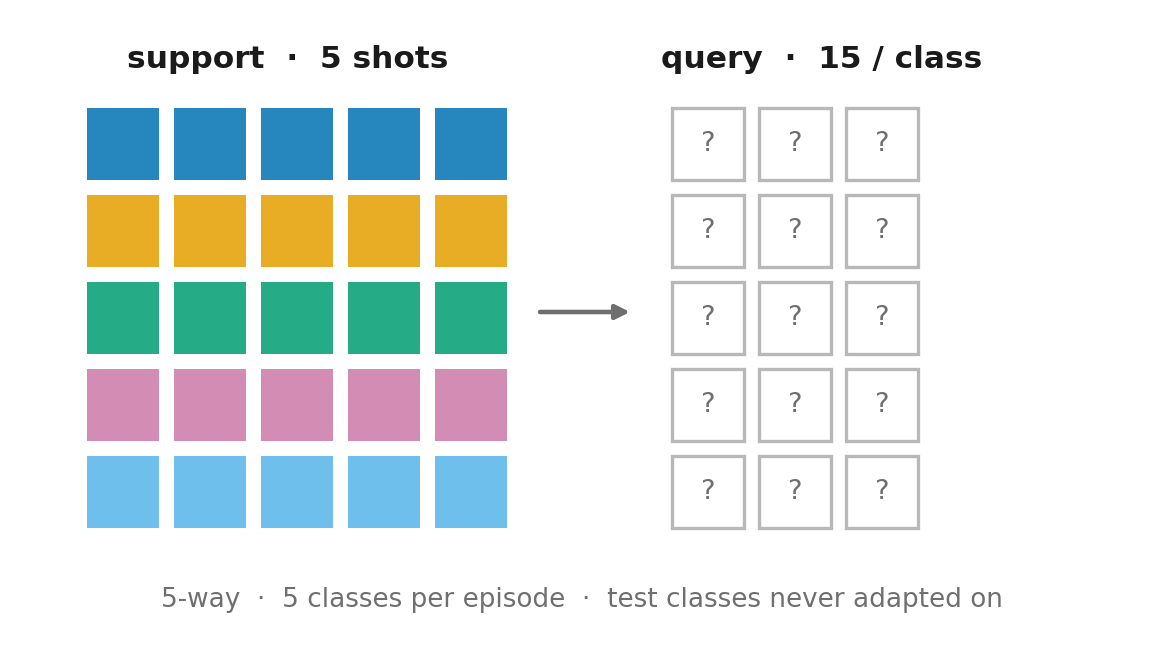
\includegraphics[width=0.7\textwidth]{figures/F2_few_shot_episode_compact.png}
    \caption{One 5-way, 5-shot episode: a support grid of 5 labelled images per class, and a query block of 15 unlabelled images per class to be classified. A fresh set of 5 classes is sampled for every episode, and the 20 test classes are never used to train the adapter.}
    \label{fig:few-shot-episode}
\end{figure}

\begin{itemize}
    \item \textbf{Task format.} 5-way $\{1, 5\}$-shot classification: each episode samples 5 classes, $K \in \{1, 5\}$ support images per class, and 15 query images per class to be classified.
    \item \textbf{Test episodes.} 600 episodes are sampled once, with their random seeds frozen in a version-controlled configuration file (\texttt{configs/test\_episodes.yaml}, seeds 0--599) that is never regenerated, so that every reported test-time number in this thesis is computed over an identical set of episodes.
    \item \textbf{Validation episodes.} A disjoint set of episodes, seeded separately (\texttt{configs/val\_episodes.yaml}, seeds 10000--10099), is used for early stopping during meta-training and for any hyperparameter selection (\autoref{sec:method-implementation}) — the 600 frozen test seeds are never used for model or hyperparameter selection, only for final reporting.
    \item \textbf{Training seeds.} Each configuration is meta-trained under 3 independent random seeds (42, 43, 44), and accuracy, calibration, and OOD numbers are reported both as a per-run 95\% confidence interval over the 600 test episodes and as the standard deviation of the per-seed means, the latter being the correct quantity for judging whether two configurations differ by more than seed noise (\autoref{chapter:results}).
    \item \textbf{Class disjointness.} The 5 classes sampled for any test episode are drawn from the 20 held-out test classes of the relevant split, which are disjoint from the 64 classes used for meta-training the adapter.
\end{itemize}

\section{Evaluation Metrics}
\label{sec:proto-metrics}

\subsection{Accuracy and Macro-F1}

Top-1 accuracy and macro-averaged F1 score are computed per episode and averaged over the 600 test episodes. In a balanced 5-way episode the two track each other closely; the gap between them, which widens specifically at 1-shot, measures per-class imbalance in the errors — with only one support image per class, a single badly-placed prototype produces a recall collapse on that one class that macro-F1 penalises more heavily than accuracy does.

\subsection{Calibration}

The Expected Calibration Error (ECE) partitions predictions into $M$ equal-width confidence bins $B_1, \dots, B_M$ and measures the average, bin-size-weighted gap between each bin's accuracy and its mean predicted confidence:
\begin{equation}
    \mathrm{ECE} = \sum_{m=1}^{M} \frac{|B_m|}{n} \, \left| \mathrm{acc}(B_m) - \mathrm{conf}(B_m) \right|.
    \label{eq:ece}
\end{equation}
Two variants are reported: \emph{pooled} ECE, computed over all query predictions from all 600 episodes pooled together, and \emph{per-episode} ECE, computed inside each episode separately and then averaged — a harsher, small-sample-sensitive variant, since a single episode contributes only 75 query predictions to its own calibration estimate. Temperature-scaled ECE is additionally reported for softmax-head configurations, following \textcite{guo2017calibration}; temperature scaling is not defined for the evidential head's Dirichlet evidence mapping and is therefore reported as not applicable in that case (\autoref{sec:method-evidence-affine} describes the evidential head's own post-hoc recalibration mechanism instead). The multi-class Brier score,
\begin{equation}
    \mathrm{BS} = \frac{1}{N} \sum_{i=1}^{N} \sum_{k=1}^{K} \left( p_{i,k} - y_{i,k} \right)^2,
    \label{eq:brier}
\end{equation}
is reported alongside ECE as a proper scoring rule that is sensitive to the full predictive distribution rather than only its maximum entry.

\subsection{Out-of-Distribution Detection}

For a chosen uncertainty score (\autoref{sec:method-ood-scores}), OOD-detection quality is measured by the Area Under the Receiver Operating Characteristic curve (AUROC) for separating in-distribution query embeddings from an OOD pool's embeddings, and by the False Positive Rate at 95\% True Positive Rate (FPR@95\%TPR) — the fraction of OOD samples incorrectly retained as in-distribution when the detection threshold is set to keep 95\% of genuine in-distribution samples. Higher AUROC and lower FPR@95 both indicate better OOD separation.

\subsection{Efficiency}

Trainable-parameter count (and, where relevant, its percentage of the frozen backbone's total parameter count), inference latency, and peak memory are reported for the efficiency and Pareto-frontier analysis (\autoref{sec:results-implications}).


% =======================================================================
\chapter{Proposed Methodology}
\label{chapter:methodology}
% =======================================================================

\section{Overview of the Methodology}
\label{sec:method-overview}

B-PEFT's architecture is a three-stage pipeline, illustrated in \autoref{fig:pipeline}: a frozen, ImageNet-pretrained CNN backbone extracts image embeddings; a small trainable adapter reshapes those embeddings for the current task, and is the \emph{only} component of the pipeline whose parameters are updated (with the sole exception of the Full-Fine-Tuning baseline, \autoref{sec:method-adapters}); and a parameter-free prototype head classifies a query image by its similarity to each class's support-set prototype, producing raw similarity logits that are then read in one of two ways — as ordinary softmax probabilities, or as evidence for a Dirichlet distribution yielding a principled uncertainty score. Each stage is described in the sections that follow, in the order data flows through them, followed by how the pipeline is trained (\autoref{sec:method-training}), how its evidential head is recalibrated after training (\autoref{sec:method-evidence-affine}), how OOD detection is scored (\autoref{sec:method-ood-scores}), and how the experimental grid itself is designed (\autoref{sec:method-grid-design}).

\begin{figure}[H]
    \centering
    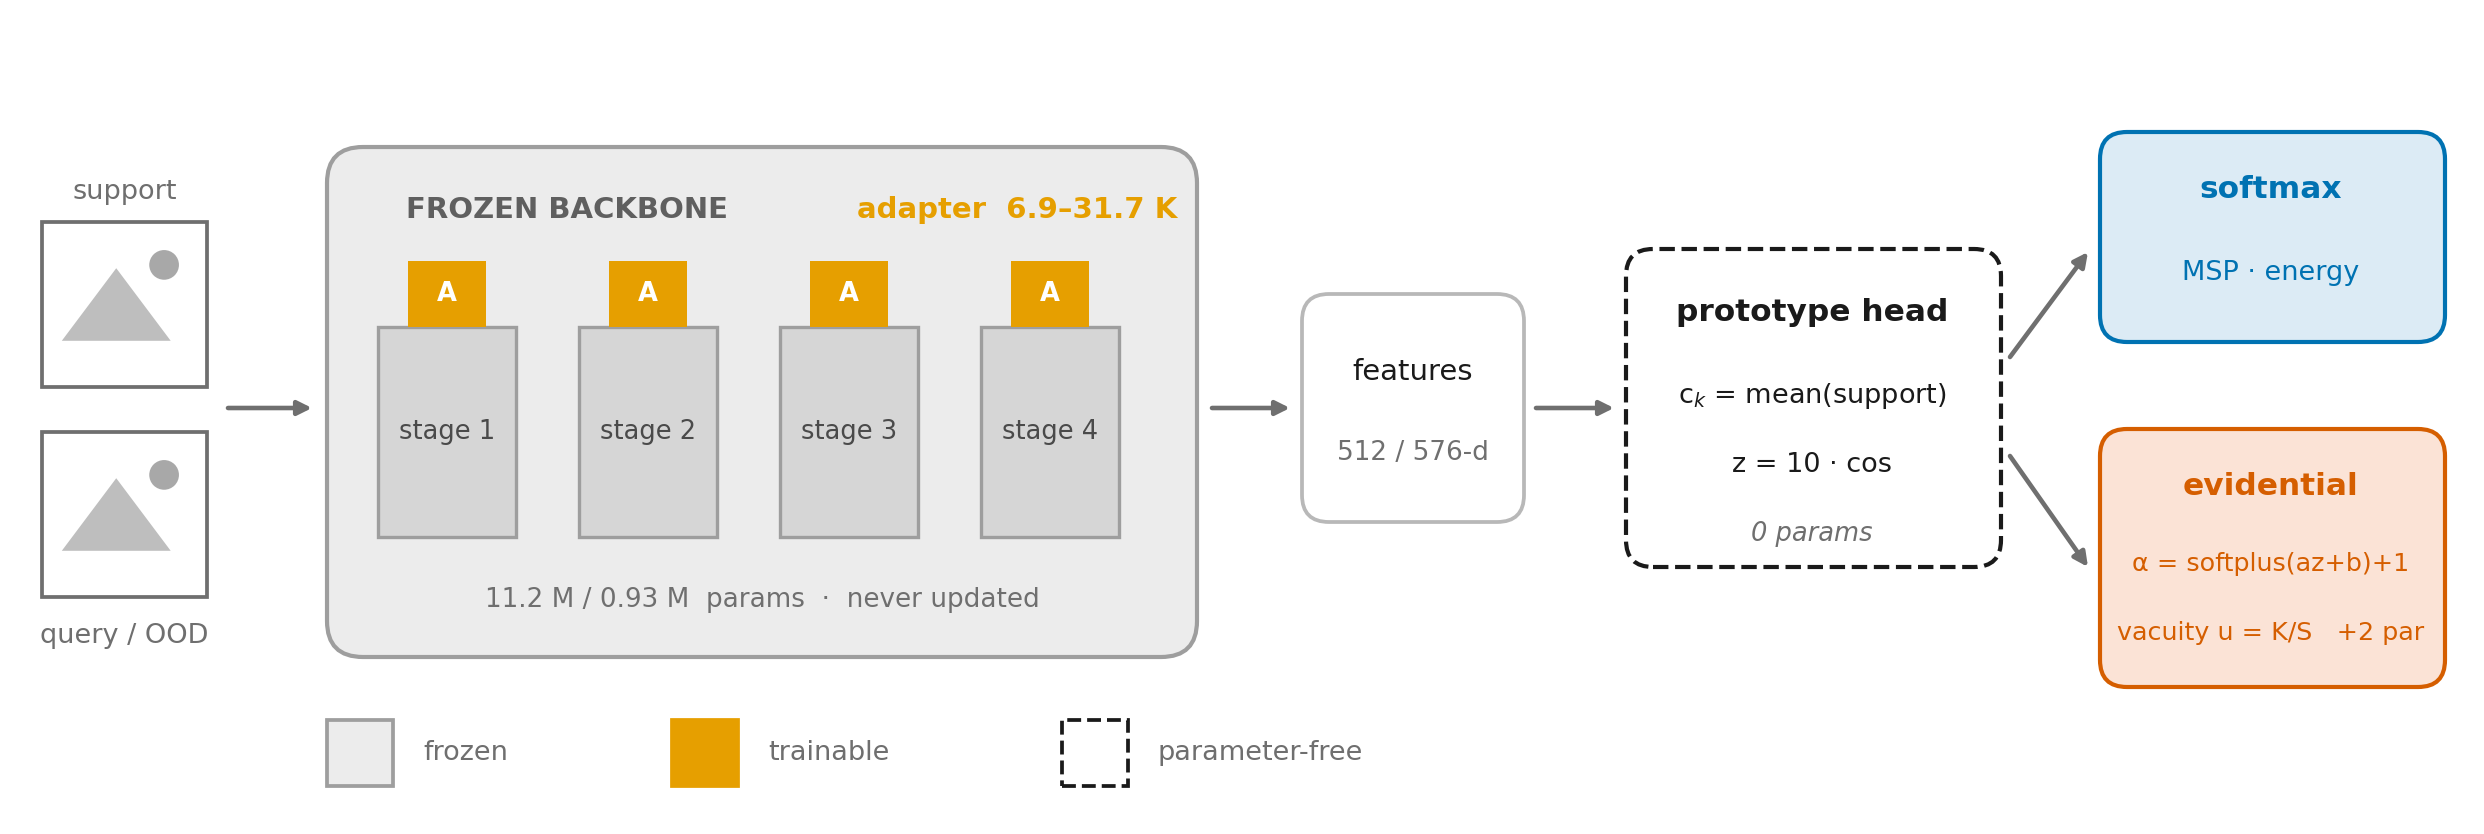
\includegraphics[width=\textwidth]{figures/F4_architecture_pipeline.png}
    \caption{The B-PEFT pipeline. Support and query images pass through the frozen backbone with a small trainable adapter inserted at each stage; the resulting features feed a parameter-free prototype head, whose similarity logits are read as either softmax or evidential (Dirichlet) probabilities. Only the adapter (orange) and, in the evidential interpretation, its two evidence-affine parameters are trained; the backbone (grey) is frozen and the prototype head has no learnable weights of its own.}
    \label{fig:pipeline}
\end{figure}

\section{Parameter-Efficient Adapters}
\label{sec:method-adapters}

Five adaptation mechanisms are compared, chosen to span the space from zero trainable parameters to full fine-tuning:

\paragraph{Bottleneck adapter~\cite{houlsby2019adapters}.} A down-projection to a bottleneck dimension $r \ll d$, a ReLU non-linearity, and an up-projection back to the original feature dimension $d$:
\begin{equation}
    \mathrm{Adapter}(x) = W_{\text{up}} \, \mathrm{ReLU}\!\left( W_{\text{down}} \, x \right), \qquad W_{\text{down}} \in \mathbb{R}^{r \times d}, \; W_{\text{up}} \in \mathbb{R}^{d \times r}.
    \label{eq:bottleneck}
\end{equation}
Following the serial/parallel vocabulary of \textcite{he2022unified}, this thesis tests both placements: \emph{serial}, where the adapter output replaces or follows the block's own output in sequence, and \emph{parallel}, where the adapter is computed from the block's \emph{input} and its output is summed into the block's output as an additional residual branch. Which placement to adopt as the standing default for the rest of the grid was settled by a single, four-configuration pilot (bottleneck adapters, serial or parallel, crossed with both head interpretations, on CIFAR-FS with ResNet-18 only, at identical trainable-parameter counts since placement changes only where the adapter's output is summed, not its size): the two placements tie on accuracy (evidential 0.915 either way; softmax 0.913 either way), but parallel is meaningfully better calibrated for the softmax head (ECE 0.063 versus 0.081) and gives substantially higher far-OOD AUROC for the evidential head (SVHN 0.933 versus 0.889), with near-OOD closely matched. On the strength of this pilot, the adapter is inserted at the final residual block of each of the four stages of ResNet-18 (and the corresponding stages of MobileNetV3-Small) in the \emph{parallel} configuration throughout the main 120-run grid, which therefore never re-tests placement at scale — this pilot, not a larger internal study, is the placement evidence this thesis's own protocol rests on; \autoref{sec:related-positioning} discusses how it relates to the much larger placement study of \textcite{li2022tsa}. Following \textcite{chen2024convadapter}'s locality caveat, this thesis's bottleneck projections use $1{\times}1$ convolutions applied per spatial location rather than a fully-connected layer over a flattened feature map, preserving the spatial locality a CNN's inductive bias depends on.

\paragraph{LoRA~\cite{hu2022lora}.} A low-rank update to a single $1{\times}1$ convolutional kernel within the backbone,
\begin{equation}
    W_{\text{new}} = W_{\text{frozen}} + A B, \qquad A \in \mathbb{R}^{d_{\text{out}} \times r}, \; B \in \mathbb{R}^{r \times d_{\text{in}}},
    \label{eq:lora}
\end{equation}
following the convolutional form of LoRA developed by \textcite{aleem2024convlora} and \textcite{zhong2024convlorasam} rather than the fully-connected form LoRA was originally proposed for. Because the target convolution is $1{\times}1$, the update itself — low-rank or not — still preserves per-pixel spatial locality, so it does not straightforwardly fall into the locality-loss failure mode \textcite{chen2024convadapter} describe for fully-connected-style adapters; this thesis treats the LoRA-versus-bottleneck comparison (\autoref{sec:results-rq3}) as a separate, corroborating data point rather than an instance of that already-named mechanism.

\begin{figure}[H]
    \centering
    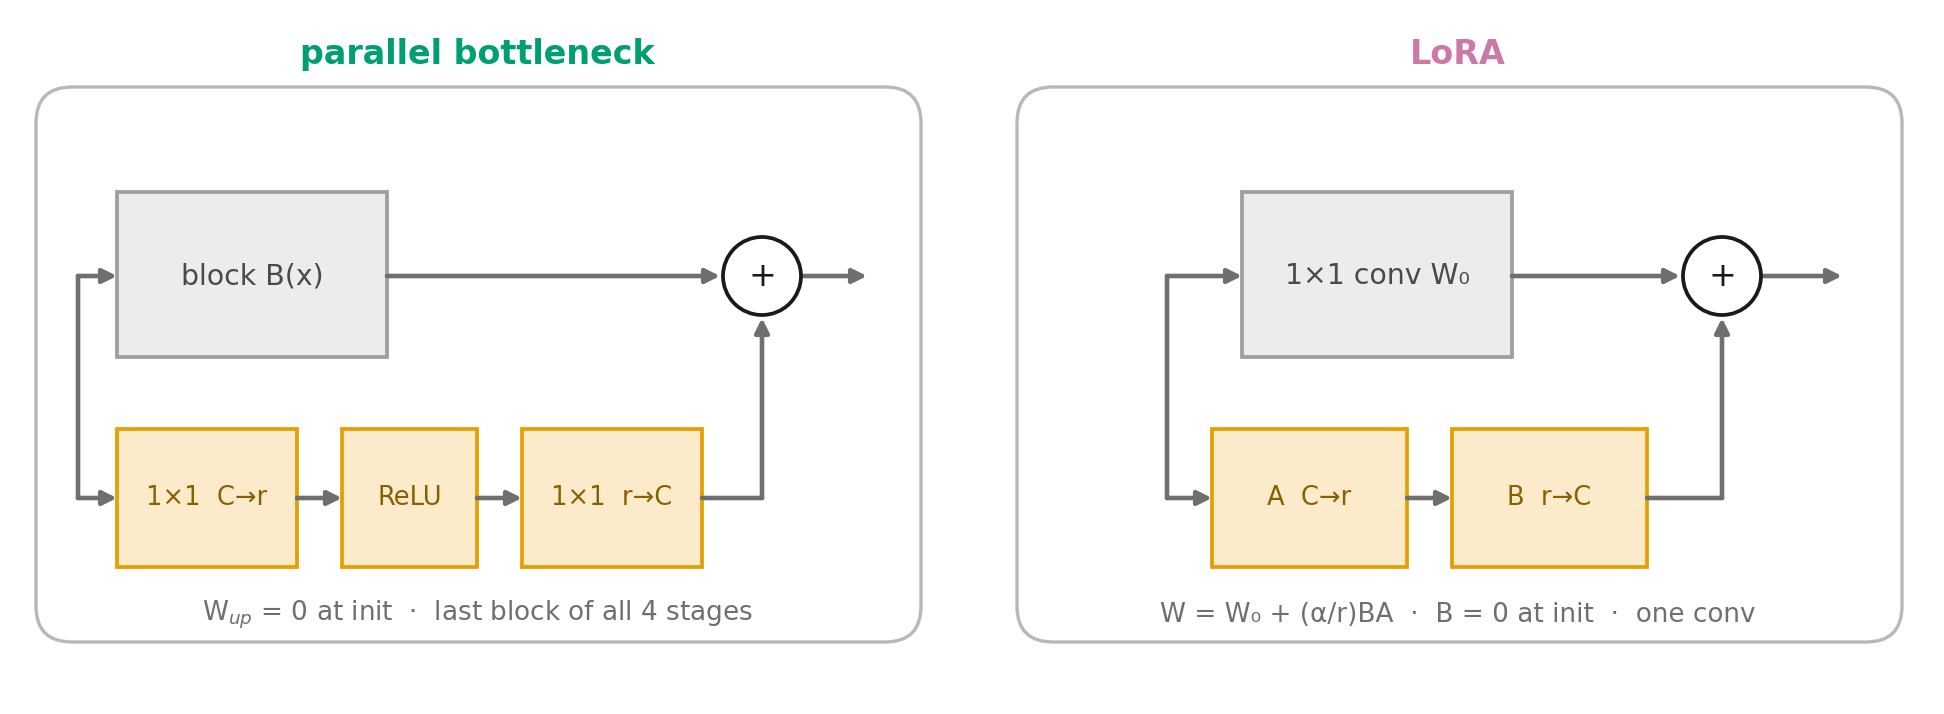
\includegraphics[width=\textwidth]{figures/F5a_adapter_zooms.png}
    \caption{The two adapter architectures compared throughout this thesis: the parallel bottleneck, a down-project/ReLU/up-project side branch added at every stage; and LoRA, a low-rank update inside a single frozen $1{\times}1$ convolution.}
    \label{fig:adapter-zooms}
\end{figure}

\paragraph{BitFit~\cite{benzaken2022bitfit}.} Only the bias terms of the backbone's convolutional and normalisation layers are unfrozen, leaving all weight tensors untouched — the most parameter-efficient mechanism tested, at under 0.1\% of the backbone's total parameters.

\paragraph{Full-Fine-Tuning (baseline).} Every backbone parameter is trainable, included as the proposal's mandatory non-PEFT reference point and as the empirical demonstration of \emph{why} PEFT is necessary in this regime: with only 5--25 labelled images per episode, full fine-tuning's 11.18-million trainable parameters (for ResNet-18) risk catastrophic overfitting, and \autoref{sec:results-param-efficiency} quantifies exactly how much accuracy and parameter cost this trades against a parameter-efficient adapter.

\paragraph{Linear-Probe (baseline).} No backbone parameter is trained at all; the frozen backbone's own features are used directly by the prototype head. Following \textcite{chen2019closerlook}'s finding that simple baselines are sometimes surprisingly competitive in low-shot regimes, this configuration is included specifically to test whether adaptation is earning its parameter cost at all — a question \autoref{sec:results-param-efficiency} answers directly.

\section{The Parameter-Free Prototype Head}
\label{sec:method-head}

Classification is performed by a Prototypical-Network-style head~\cite{snell2017protonet}: for each of the $N$ classes in an episode, a class prototype $c_n$ is computed as the mean embedding of that class's $K$ support examples,
\begin{equation}
    c_n = \frac{1}{K} \sum_{i \in \text{support}(n)} f_{\theta}(x_i),
    \label{eq:prototype}
\end{equation}
where $f_\theta$ is the frozen-backbone-plus-adapter embedding function. A query image $x$ is classified by its scaled cosine similarity to each prototype, giving one raw logit per class:
\begin{equation}
    z_n(x) = \tau \, \frac{f_\theta(x) \cdot c_n}{\lVert f_\theta(x) \rVert \, \lVert c_n \rVert}, \qquad \tau = 10.
    \label{eq:proto-logit}
\end{equation}
This head has \emph{no trainable parameters of its own}: its only dependence on the adapter is through the embedding function $f_\theta$. This design choice is deliberate rather than incidental — a trainable linear classification head, once fit to the 64 meta-training classes, has no principled way to generalise to the 20 disjoint classes seen only at test time, whereas a similarity-based head is defined for any set of classes by construction, since it only ever compares a query embedding to the prototypes computed \emph{from that same episode's} support set. This is a deliberate, documented departure from the naive reading of the original research proposal, which had assumed a trainable linear head; the switch was made once the disjoint-class evaluation protocol (\autoref{sec:proto-episodic}) made clear that a linear head trained on the 64 base classes cannot be evaluated on the 20 held-out test classes without either retraining it per episode (defeating the purpose of a frozen adaptation budget) or accepting that its logits are meaningless for classes it never saw.

Every configuration in this thesis uses scaled cosine similarity rather than the negative squared Euclidean distance \textcite{snell2017protonet} report as the stronger metric for Prototypical Networks. This is a deliberate departure, made for two reasons rather than by default: raw Euclidean-distance logits from a ResNet-18 embedding are large and negative, which is precisely what collapsed the evidential mapping in \autoref{sec:method-evidence-affine} before the affine rescaling was introduced, whereas cosine similarity is bounded in $[-\tau, \tau]$ by construction; and using the same metric for both head interpretations keeps the softmax-versus-evidential comparison from being confounded with a metric choice as well. Cosine-similarity prototype classifiers are themselves a standard few-shot baseline, following \textcite{chen2019closerlook}'s cosine-similarity classifier. No Euclidean-distance run was repeated under this thesis's final training recipe, so the accuracy cost of this choice relative to the metric \textcite{snell2017protonet} recommend is not separately measured here and is stated as an open question rather than assumed to be negligible.

\section{From Logits to Belief: Softmax versus Evidential Interpretation}
\label{sec:method-evidence-affine}

The prototype head's raw logits $z_n(x)$ from \autoref{eq:proto-logit} are, by design, a fixed quantity computed identically regardless of what happens next; \emph{head interpretation} is a separate design axis (\autoref{sec:method-grid-design}) that decides how those logits are read.

\subsection{Softmax interpretation}

The standard reading: $\hat p_n = \mathrm{softmax}(z)_n$, with prediction confidence given by the maximum softmax probability (MSP, \autoref{sec:method-ood-scores}).

\subsection{Evidential (Dirichlet) interpretation}

\begin{figure}[H]
    \centering
    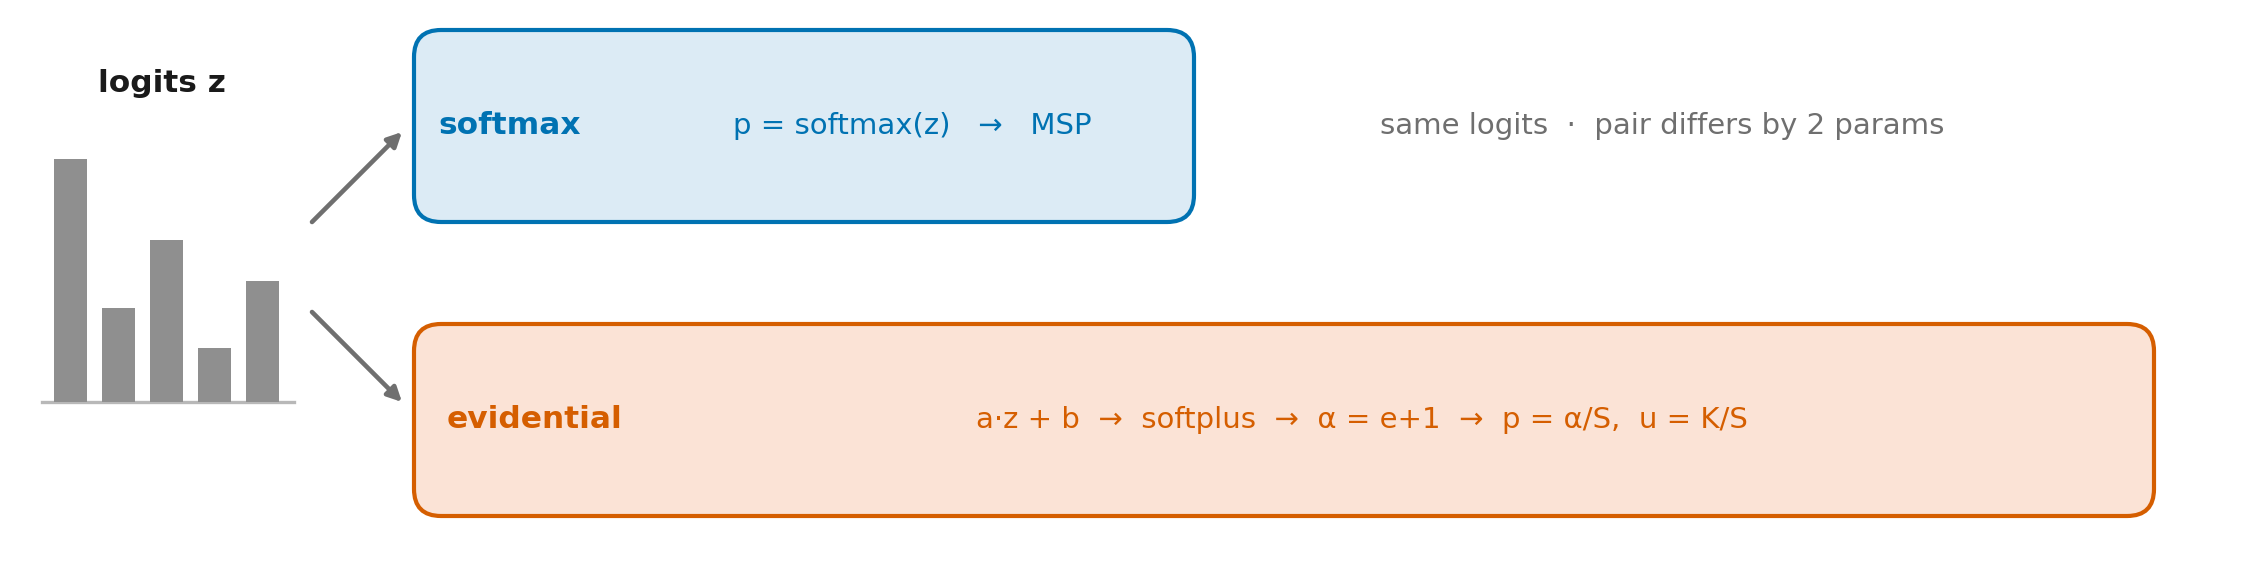
\includegraphics[width=0.85\textwidth]{figures/F6a_head_two_readouts.png}
    \caption{One set of raw similarity logits, read two ways: softmax probabilities scored by MSP/energy, or Dirichlet evidence scored by vacuity. The two interpretations differ by exactly the two evidence-affine parameters.}
    \label{fig:head-two-readouts}
\end{figure}

Following \textcite{sensoy2018edl}, the logits are instead mapped to non-negative \emph{evidence} $e_n$ for each class, from which Dirichlet concentration parameters $\alpha_n = e_n + 1$ are formed, giving total Dirichlet strength $S = \sum_n \alpha_n$, predictive probability $\hat p_n = \alpha_n / S$, and epistemic uncertainty (vacuity) $u = K/S$ for $K = 5$ classes — a network with little evidence for any class produces small $S$ and therefore high vacuity, independent of how that scant evidence happens to be distributed among the $N$ classes.

The mapping from logit to evidence is the single most consequential implementation detail in this thesis, and it is worth explaining why. The originally proposed mapping, following EDL's presentation in general terms, was $e_n = \mathrm{ReLU}(z_n)$. Applied directly to this thesis's similarity-based logits from \autoref{eq:proto-logit}, this mapping fails silently: negative-squared-distance logits from a ResNet-18 embedding space are large in magnitude and almost always negative, so $\mathrm{ReLU}(z_n) = 0$ for essentially every class in essentially every episode, collapsing the Dirichlet distribution to uniform ($\alpha_n = 1$ for all $n$) regardless of the input, and producing dead gradients throughout training. This is exactly the class of failure the project's implementation guidance warns to watch for: a mechanism drawn correctly from its source paper, but silently broken by an assumption (small-magnitude, sign-mixed logits) that does not hold for this thesis's specific head design. The corrected mapping introduces a learned affine rescaling before the non-linearity, and replaces $\mathrm{ReLU}$ with the strictly-positive, smooth $\mathrm{softplus}$:
\begin{equation}
    e_n = \mathrm{softplus}\!\left( z_n \cdot \mathrm{scale} + \mathrm{bias} \right), \qquad \alpha_n = e_n + 1, \qquad S = \sum_{n} \alpha_n, \qquad u = \frac{K}{S}.
    \label{eq:evidence-affine}
\end{equation}
The two parameters $\mathrm{scale}$ and $\mathrm{bias}$ are the \emph{only} trainable parameters this mapping adds — exactly two — which is why an evidential-head configuration's trainable-parameter count is always two more than the corresponding softmax-head configuration's (for example, 31{,}746 versus 31{,}744 for the ResNet-18 parallel-bottleneck adapter). This mapping — \autoref{eq:evidence-affine} — is implemented once and shared, by design, between the training loss and the evaluator's OOD scoring code, specifically so that the two can never silently drift apart and reintroduce the same collapse failure in only one of the two consumers.

\begin{table}[H]
    \centering
    \small
    \begin{tabular}{lll}
        \toprule
        & Softmax & Evidential (Dirichlet) \\
        \midrule
        Output & Class probabilities & Evidence $\to$ Dirichlet $\to$ probabilities \\
        Uncertainty signal & Maximum probability (MSP) & Vacuity (``I don't know'') \\
        Extra parameters & 0 & 2 (learnable scale and bias) \\
        \bottomrule
    \end{tabular}
    \caption{The two head interpretations compared. Both read the same underlying similarity logits (\autoref{eq:proto-logit}); they differ only in the transform applied afterward and its two extra parameters.}
    \label{tab:head-comparison}
\end{table}

\section{The Evidential Training Objective}
\label{sec:method-evidential-loss}

Following \textcite{sensoy2018edl}, the evidential head is trained with the Type-II maximum-likelihood evidential loss — the expected sum-of-squares error of the predicted Dirichlet mean against the one-hot label, marginalised over the Dirichlet distribution itself — plus a Kullback--Leibler divergence term that regularises the \emph{evidence} for incorrect classes toward zero, i.e.\ toward the uniform Dirichlet prior, for correctly-classified examples only. \textcite{gao2024edlsurvey} document the standard design rationale for this KL term: without it, the evidential loss alone has no mechanism preventing the network from accumulating spurious evidence for wrong classes, since spreading evidence across all classes proportionally does not change the predicted mean. Because applying the full KL penalty from the first training step can suppress the network from producing \emph{any} confident evidence before it has learned to discriminate between classes at all, the KL term's weight is annealed in from zero over the early part of training rather than applied at full strength immediately — a stabilisation this project's own early development history (an initial configuration that disabled the KL term entirely and used cross-entropy directly on the softplus evidence) showed to be necessary empirically, not merely as a theoretical nicety: correcting this single issue, together with the ReLU-to-softplus change of \autoref{eq:evidence-affine}, reduced this system's ECE by close to an order of magnitude in an early single-episode pilot, before the project moved to the full episodic protocol used for every result in \autoref{chapter:results}.

\section{Episodic Meta-Training Procedure}
\label{sec:method-training}

The adapter (and, in the evidential configuration, the two evidence-affine parameters) is meta-trained by sampling many episodes per epoch from the 64 meta-training classes, in each case: (1) computing the embedding, via the frozen backbone plus the current adapter, of every support and query image in the sampled episode; (2) computing class prototypes from the support embeddings (\autoref{eq:prototype}); (3) computing query logits by similarity to each prototype (\autoref{eq:proto-logit}); (4) computing the training loss appropriate to the configured head interpretation (\autoref{sec:method-evidential-loss} for evidential, standard cross-entropy for softmax); and (5) backpropagating through the adapter only, since the backbone is frozen and the prototype head has no parameters of its own. This is repeated for many sampled episodes per epoch, with performance on a fixed stream of validation episodes (\autoref{sec:proto-episodic}) checked after every epoch and training stopped once validation accuracy plateaus. This \emph{episodic} meta-training procedure, introduced to the project from Step 4 onward, replaced an earlier, simpler single-fixed-episode procedure used in the project's first three development steps, in which 200 direct gradient steps were taken on one fixed episode with no meta-training across episodes at all; the earlier procedure is retained in the codebase for reproduction purposes but is not the source of any result reported in \autoref{chapter:results}, all of which use the true episodic procedure described here.

\section{Post-Hoc Recalibration of the Evidential Head}
\label{sec:method-recalibration}

The two evidence-affine parameters of \autoref{eq:evidence-affine} — $\mathrm{scale}$ and $\mathrm{bias}$ — are \emph{not} frozen: they are initialised at $(2, -6)$ and learned jointly with the adapter during meta-training, the same as any other trainable parameter in that configuration. Across the evidential checkpoints in the main grid they move to a range of roughly $\mathrm{scale} \in [1.5, 4.5]$ and $\mathrm{bias} \in [-9.3, -5.6]$ — i.e.\ every configuration ends training at its own point, not at the shared initial value. RQ4 (\autoref{sec:results-rq4}) asks a distinct question: if these two parameters are instead \emph{refit after training}, holding the adapter itself fixed, on that configuration's own validation episodes, does the evidential head's calibration improve further beyond wherever joint training already left it — and, since the affine transform is monotone in each \emph{individual} logit but vacuity ($u = K/S$) is a function of \emph{all} $K$ logits jointly, does the head's OOD ranking survive the refit? Unlike temperature scaling for a softmax head, which is provably rank-preserving because it is a single monotone transform of the arguments to a rank-invariant $\arg\max$, no such guarantee holds here a priori, so whether ranking is preserved is treated in this thesis as an empirical question to be measured (\autoref{sec:results-rq4}), not assumed.

\section{Out-of-Distribution Scoring Rules}
\label{sec:method-ood-scores}

Four uncertainty scores are computed and compared throughout this thesis, following \textcite{yang2022openood}'s near/far taxonomy for the OOD pools they are evaluated against (\autoref{sec:proto-datasets}):

\begin{itemize}
    \item \textbf{Vacuity} ($u = K/S$, evidential head only) — this thesis's primary evidential uncertainty score, as derived in \autoref{sec:method-evidence-affine}.
    \item \textbf{Maximum softmax probability (MSP)}~\cite{hendrycks2017baseline} — the softmax head's standard confidence score, $\max_n \hat p_n$.
    \item \textbf{Temperature-scaled MSP (TS-MSP)} — MSP computed after fitting a single scalar temperature on the validation split, following \textcite{guo2017calibration}.
    \item \textbf{Energy}~\cite{liu2020energy} — a training-free score computed directly from the raw logits, $-\log \sum_n \exp(z_n)$, requiring no probabilistic interpretation of the head at all.
\end{itemize}

Because the base experimental grid scores evidential-head runs with vacuity only and softmax-head runs with MSP, TS-MSP, and energy only, every naturally-arising comparison in the grid varies the training objective (evidential versus softmax) and the scoring rule \emph{together}; RQ2 (\autoref{sec:results-rq2}) is designed specifically to break this confound by computing all four scores on all runs regardless of which head trained them.

\section{Experimental Design}
\label{sec:method-grid-design}

\subsection{The main grid}

The main experimental grid crosses five binary or near-binary design axes into a balanced $2^5$ full factorial of 32 cells, plus 8 additional baseline cells that are not part of the balanced factorial:

\begin{itemize}
    \item \textbf{Dataset} $\in \{$CIFAR-FS, MiniImageNet$\}$
    \item \textbf{Shots} $\in \{1, 5\}$
    \item \textbf{Backbone} $\in \{$ResNet-18, MobileNetV3-Small$\}$
    \item \textbf{Adapter} $\in \{$Bottleneck-parallel, LoRA$\}$ (the balanced factorial; Full-Fine-Tuning and Linear-Probe appear only as unbalanced baseline cells on CIFAR-FS $\times$ ResNet-18)
    \item \textbf{Head interpretation} $\in \{$Softmax, Evidential$\}$
\end{itemize}

giving $2 \times 2 \times 2 \times 2 \times 2 = 32$ balanced cells plus $2$ (baseline adapters) $\times 2$ (heads) $= 4$... and, because both Full-Fine-Tuning and Linear-Probe are additionally run at both shot counts, $8$ baseline cells in total, for $40$ unique configurations. Each configuration is meta-trained under 3 seeds (42, 43, 44), giving $40 \times 3 = 120$ completed runs, all evaluated over the identical frozen 600-episode test stream (\autoref{sec:proto-episodic}) under a single hyperparameter recipe fixed once in advance and never re-tuned per cell — the grid therefore answers ``how do these design axes compare under one fixed recipe,'' not ``what is the best achievable number in each cell,'' a scope limitation this thesis states explicitly rather than leaving implicit (\autoref{sec:results-limitations}).

\begin{figure}[H]
    \centering
    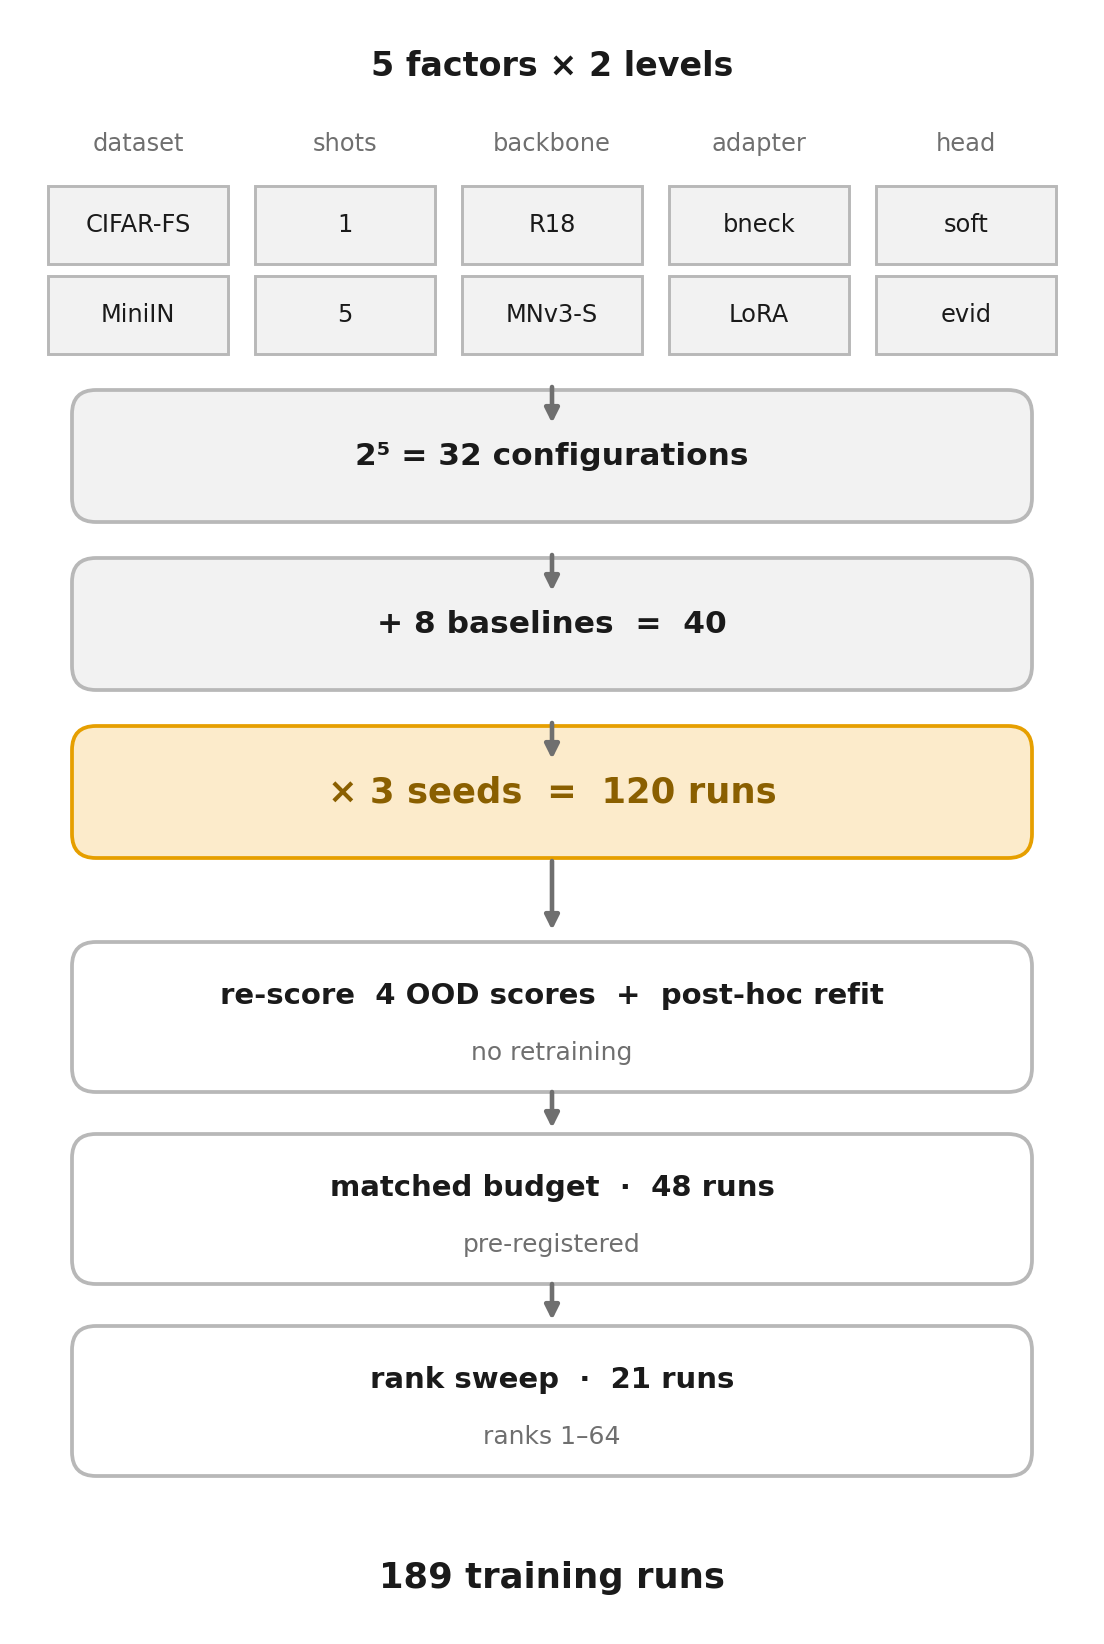
\includegraphics[width=0.6\textwidth]{figures/F7_experimental_design_flow.png}
    \caption{The full experimental design: the base grid (120 runs), re-scored with 4 OOD scores and a post-hoc refit at no extra training cost, followed by the matched-budget experiment (48 runs) and the rank sweep (21 runs) — 189 training runs in total.}
    \label{fig:experimental-design-flow}
\end{figure}

A structural fact about this grid makes RQ3 possible. The trainable-parameter counts of the two balanced-factorial adapters are:

\begin{table}[H]
    \centering
    \small
    \begin{tabular}{lrr >{\raggedright\arraybackslash}p{3.4cm}}
        \toprule
        Backbone & Bottleneck-parallel & LoRA & Larger adapter \\
        \midrule
        ResNet-18 & 31{,}744 & 12{,}288 & Bottleneck, by 2.58$\times$ \\
        MobileNetV3-Small & 6{,}928 & 10{,}752 & LoRA, by 1.55$\times$ \\
        \bottomrule
    \end{tabular}
    \caption{Trainable-parameter counts (softmax head; the evidential head adds exactly 2 to each cell) for the two balanced-factorial adapters, by backbone. The ordering reverses between backbones.}
    \label{tab:param-reversal}
\end{table}

The larger adapter is bottleneck on ResNet-18 but LoRA on MobileNetV3-Small — a reversal that falls out of the two backbones' channel widths rather than being designed in, and that partially deconfounds adapter \emph{architecture} from adapter \emph{parameter budget}, which is normally impossible in a PEFT study because the more accurate adapter is usually also the larger one everywhere. \autoref{sec:results-rq3} shows why this reversal, while informative, is not sufficient on its own to fully separate the two explanations, and why a dedicated follow-up experiment was required.

\subsection{The matched-budget follow-up experiment}
\label{sec:method-matched-budget}

Because the parameter-budget reversal in \autoref{tab:param-reversal} is welded to the choice of backbone, a finding of the form ``the larger-budget adapter is better calibrated'' and a finding of the form ``something about the backbone determines calibration'' predict the \emph{identical} 16-pair pattern in the base grid — the two explanations cannot be told apart by that data alone. To adjudicate between them, a second, pre-registered experiment was designed and run: both adapter architectures are rebuilt at the \emph{same} trainable-parameter budget \emph{within} each backbone (rather than relying on the accidental cross-backbone reversal), at two budget levels per backbone, on MiniImageNet 5-shot, with both head interpretations trained separately and 3 seeds each, for $2~\text{backbones} \times 2~\text{levels} \times 2~\text{adapters} \times 2~\text{heads} \times 3~\text{seeds} = 48$ runs. The decision rule for adjudicating between the budget hypothesis and the backbone-intrinsic hypothesis was fixed \emph{before} the 48 runs were executed, so that the result reported in \autoref{sec:results-matched-budget} is a genuine test rather than a post-hoc rationalisation of whichever pattern happened to appear. Residual parameter-count mismatch between the matched pairs is kept under 3.10\%, against 55--158\% mismatch in the original 16-pair comparison, making this experiment a substantially tighter test of the budget hypothesis than the base grid alone could provide.

\section{Implementation and Reproducibility}
\label{sec:method-implementation}

The system is implemented as a configuration-driven codebase: every experiment is specified by a YAML configuration file that may \texttt{extend} a parent configuration (recursively deep-merged, with the child's keys taking precedence), so that each of the 40-plus experiment configurations used in this thesis need only state what differs from a shared base configuration rather than repeating every hyperparameter. Two command-line entry points, a training script and an evaluation script, consume these configurations and dispatch to the appropriate adapter, head, and trainer implementation via a small factory function per component, so that adding a new adapter or head variant requires adding one class and one branch in that component's factory rather than modifying any calling code. Every run seeds Python, NumPy, and PyTorch's CPU and CUDA random-number generators and forces deterministic cuDNN behaviour, so that re-running the identical configuration reproduces a byte-identical result file; this determinism is checked as a standing convention rather than asserted once and forgotten; two of the forty configurations in this grid (Full-Fine-Tuning and Linear-Probe) additionally have \emph{zero} across-seed variance by construction, since Full-Fine-Tuning starts from the same pretrained weights regardless of seed and Linear-Probe has no trainable parameters for a seed to perturb at all — a fact this thesis's own interpretation of those two baselines' results accounts for explicitly (\autoref{sec:results-limitations}) rather than treating their 3 nominal seeds as 3 independent observations. Experiment tracking is handled uniformly across online, offline, and fully-disabled modes by a thin wrapper, with logging disabled by default so that a run produces no tracking-service side effects unless explicitly requested. All training in this thesis was carried out on cloud GPU instances (Google Colab and Kaggle, predominantly NVIDIA Tesla T4 hardware); no local GPU hardware was used, and the efficiency measurements reported in \autoref{sec:results-implications} are explicitly qualified by which hardware profile they were measured on, after an earlier internal error in which several plotting scripts silently selected the wrong latency profile was caught and corrected.


% =======================================================================
\chapter{Results and Discussion}
\label{chapter:results}
% =======================================================================

This chapter reports every result the thesis rests on. It opens with the parameter-efficiency comparison that motivates parameter-efficient adaptation in the first place, then addresses the four research questions of \autoref{sec:intro-rqs} in turn, each built on the 120-run grid plus the dedicated matched-budget follow-up (\autoref{sec:method-matched-budget}) where relevant. It closes with the measured deployment-cost implications, the system's positioning against comparable published work (\autoref{sec:results-positioning}), and the study's limitations stated without euphemism (\autoref{sec:results-limitations}).

\section{Overview of the Experiment Grid}

\autoref{tab:grid-recap} recaps the grid design of \autoref{sec:method-grid-design}: 40 unique configurations (32 in a balanced factorial plus 8 unbalanced baseline cells), each run under 3 seeds, for 120 completed training runs, every one evaluated on the identical frozen 600-episode test stream. The complete result tables — accuracy, macro-F1, and trainable-parameter count (\autoref{tab:apx-accuracy}); calibration (\autoref{tab:apx-calibration}); OOD AUROC (\autoref{tab:apx-auroc}); and OOD FPR@95\%TPR (\autoref{tab:apx-fpr95}) — are reproduced in full in \autoref{apx:results}; this chapter presents the subsets and derived statistics needed to answer each research question in turn.

\begin{table}[H]
    \centering
    \small
    \begin{tabular}{>{\raggedright\arraybackslash}p{3cm} >{\raggedright\arraybackslash}p{10.5cm}}
        \toprule
        Axis & Values \\
        \midrule
        Dataset & CIFAR-FS, MiniImageNet \\
        Shots & 1-shot, 5-shot (5-way throughout) \\
        Backbone & ResNet-18, MobileNetV3-Small (both frozen, ImageNet-pretrained) \\
        Adapter & Bottleneck-parallel, LoRA, Full-FT*, Linear-Probe* (* baseline, CIFAR-FS/ResNet-18 only) \\
        Head interpretation & Evidential (Dirichlet), Softmax \\
        Seeds & 42, 43, 44 \\
        \bottomrule
    \end{tabular}
    \caption{The experimental grid: 40 unique configurations $\times$ 3 seeds = 120 runs.}
    \label{tab:grid-recap}
\end{table}

\section{Results: Parameter Efficiency}
\label{sec:results-param-efficiency}

At 5-shot, the 31{,}744-parameter parallel-bottleneck adapter on ResNet-18 \emph{beats} the 11{,}176{,}512-parameter Full-Fine-Tuning baseline outright (91.44\% versus 90.47\% accuracy, \autoref{tab:apx-accuracy}) — 352$\times$ fewer trainable parameters for higher accuracy — direct empirical support for this thesis's central premise that full fine-tuning is not merely unnecessary but actively counterproductive in this data regime. The Linear-Probe baseline, with zero trainable adapter parameters, still reaches a respectable 87.41\% at 5-shot, confirming \textcite{chen2019closerlook}'s observation that a simple baseline is a real contender in low-shot settings, but it is decisively beaten by every adapter tested, so adaptation is earning its parameter cost.

\begin{figure}[H]
    \centering
    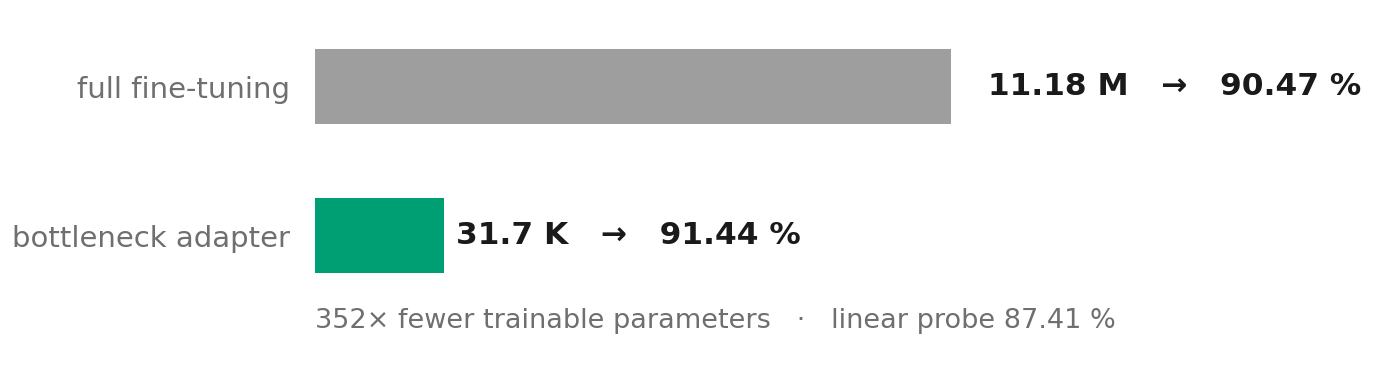
\includegraphics[width=0.8\textwidth]{figures/D2_parameter_efficiency_bars.png}
    \caption{Full fine-tuning versus the parallel-bottleneck adapter versus the linear probe: trainable parameters and accuracy, CIFAR-FS 5-shot, ResNet-18.}
    \label{fig:param-efficiency-bars}
\end{figure}

\section{RQ1: Attribution of Outcome Variance Across Design Axes}
\label{sec:results-rq1}

Main-effect $\eta^2$ (share of total variance explained) was computed over the balanced $2^5$ factorial on all 96 per-seed observations (not seed-averaged first, so that a genuine residual/error term is retained rather than mechanically suppressed):

\begin{table}[H]
    \centering
    \footnotesize
    \begin{tabular}{>{\raggedright\arraybackslash}p{3.4cm} rrrrrr}
        \toprule
        Metric & Dataset & Shots & Backbone & Adapter & Head & Residual \\
        \midrule
        Accuracy & 1.75\% & \textbf{76.05\%} & 3.92\% & 9.14\% & 0.19\% & 8.95\% \\
        ECE & 2.02\% & 2.13\% & 4.63\% & 0.63\% & \textbf{82.89\%} & 7.70\% \\
        OOD AUROC (far) & 1.18\% & 22.68\% & 11.54\% & 1.73\% & \textbf{39.01\%} & 23.87\% \\
        OOD AUROC (near, TinyImageNet) & 1.64\% & \textbf{42.60\%} & 0.61\% & 21.98\% & 20.98\% & 11.42\% \\
        \bottomrule
    \end{tabular}
    \caption{Per-seed $\eta^2$ variance decomposition (96 observations) across the five balanced-factorial design axes. Bold marks the dominant axis for each outcome.}
    \label{tab:rq1-eta2}
\end{table}

\begin{figure}[H]
    \centering
    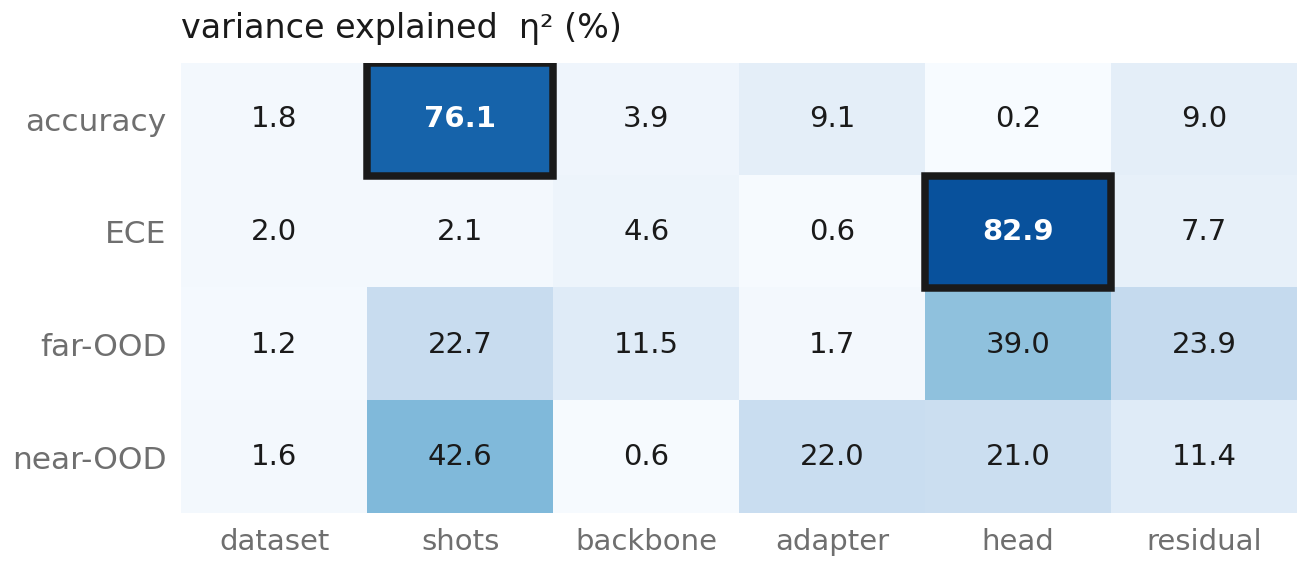
\includegraphics[width=0.85\textwidth]{figures/F11_main_effects_heatmap.png}
    \caption{Main-effects heatmap: share of variance ($\eta^2$, \%) each design axis explains for each outcome. Accuracy is dominated by shots; ECE by head; neither OOD pool has one dominant factor.}
    \label{fig:main-effects-heatmap}
\end{figure}

Two results stand out. First, \textbf{head interpretation explains roughly 83\% of calibration variance and under 0.2\% of accuracy variance} — close to a clean separation of concerns between which design choices govern accuracy and which govern calibration. This was first computed on seed-\emph{averaged} data (84.0\%/0.2\%, with residuals of only 6.5--20.3\%), and a concern was raised, informed by a contemporaneous large-scale study reporting a genuine 10.6\% per-observation residual for a similar decomposition~\cite{krumpl2026onemodel}, that averaging seeds before decomposing variance mechanically suppresses the error term and manufactures an artificially clean split. Recomputing the full decomposition on all 96 raw per-seed observations, as reported in \autoref{tab:rq1-eta2}, moves the residual by only 0.3--3.6 percentage points — nowhere near enough to explain the accuracy/calibration split as an averaging artefact. The claim holds on per-seed data. Second, across all 40 cells the rank correlation between ECE and OOD AUROC is \emph{positive} (Spearman $\rho = +0.433$ for SVHN-far, $+0.477$ for TinyImageNet-near) — worse-calibrated configurations appear, superficially, to detect OOD \emph{better}. Stratifying by head interpretation collapses this correlation to $\rho = +0.150$/$+0.195$ within the evidential head and $+0.263$/$+0.242$ within the softmax head: the apparent tension is entirely a head effect, and the defensible statement is that calibration and OOD-detection quality are \emph{orthogonal}, not that one trades against the other, once head interpretation is held fixed.

The concrete evidence behind the 83\% calibration share is a clean, decisive negative result and is worth stating in full rather than only as a percentage. Across all 20 matched evidential-versus-softmax comparisons in the balanced grid (holding dataset, shots, backbone, and adapter fixed), the evidential head's pooled ECE is \emph{worse} than the corresponding softmax head's in every single case, by factors of 1.4$\times$ to 9.1$\times$, and worse still relative to temperature-scaled softmax (5.3$\times$ to 51$\times$). \autoref{tab:head-ece-subset} reproduces a representative subset from \autoref{tab:apx-calibration}. The gap does not narrow with more support examples: at 5-shot, evidential ECE on CIFAR-FS/ResNet-18/Bottleneck-parallel is 0.3010 against a softmax ECE of 0.0670 — a widening, not narrowing, of the gap relative to 1-shot. Accuracy does not compensate for this either: in only 7 of the 20 matched pairs is the evidential head's accuracy high enough to plausibly offset its calibration cost, and even there the calibration gap remains an order of magnitude larger than the accuracy difference would justify.

\begin{table}[H]
    \centering
    \small
    \begin{tabular}{llrrr}
        \toprule
        Dataset & Shots & ECE (Evidential) & ECE (Softmax) & ECE (Softmax, temp.\ scaled) \\
        \midrule
        CIFAR-FS & 1-shot & 0.2765 & 0.0560 & 0.0297 \\
        CIFAR-FS & 5-shot & 0.3010 & 0.0670 & 0.0152 \\
        MiniImageNet & 1-shot & 0.3073 & 0.1012 & 0.0073 \\
        MiniImageNet & 5-shot & 0.2938 & 0.0850 & 0.0057 \\
        \bottomrule
    \end{tabular}
    \caption{Pooled ECE for the ResNet-18, Bottleneck-parallel configuration, evidential versus softmax (with and without post-hoc temperature scaling). Lower is better; the evidential head is worse in every row.}
    \label{tab:head-ece-subset}
\end{table}

This negative result is not an isolated artefact of this thesis's specific implementation: \textcite{bengs2022pitfalls} show theoretically that loss-minimisation-based evidential objectives of this kind can retain non-vanishing epistemic uncertainty even in the infinite-data limit, and \textcite{hoarau2026epistemic} report an independent 2026 theoretical analysis reaching a compatible conclusion for second-order (evidential) classifiers trained with a reverse-KL objective. Read together with this thesis's own 20/20 negative result, the empirical finding and the theoretical literature point the same way, and this thesis presents the negative result as convergent evidence rather than as a failed experiment to be explained away. At the same time, as \autoref{sec:results-rq2} shows next, the same evidential head that calibrates worse is simultaneously a substantially \emph{better} OOD ranker than the softmax baseline it is compared against here — the central tension RQ2 is built to resolve.

The specific analytical method here — a formal $\eta^2$ decomposition of accuracy, calibration, and OOD AUROC in a PEFT/few-shot setting — appears methodologically novel: the largest existing calibration benchmark, at 117{,}702 architectures~\cite{tao2024benchmarkcalibration}, was verified directly to run no comparable variance decomposition, using box plots and rank correlations only. The \emph{qualitative} pattern that calibration and accuracy are governed by different factors, however, is not new — it follows directly from \textcite{guo2017calibration} and \textcite{minderer2021revisiting} — and this thesis presents it as rigorous confirmation and precise quantification in a new setting, not as an independent discovery. The correlation-collapse-under-stratification result (ECE/AUROC orthogonality once head is fixed) was not found described anywhere else in the literature reviewed for this thesis and is presented as the section's genuinely new contribution.

\section{RQ2: Training Objective versus Scoring Rule}
\label{sec:results-rq2}

The motivation for this question comes from a correction the project made to its own earlier reading of the grid. Vacuity beats the softmax-probability scores (MSP and TS-MSP) in 37--38 of 40 matched cells across the full grid, by margins of $+0.045$ to $+0.141$ AUROC depending on the OOD pool — the standard, well-established evidential-uncertainty result. Against the training-free \emph{energy} score, however, the picture reverses: an earlier, single-configuration result from mid-project development had suggested vacuity was roughly on par with energy, but the full 120-run grid overturns this — vacuity beats energy in only 10 of 40 far-OOD and 14 of 40 near-OOD matched comparisons, with energy the better default OOD score in roughly 70\% of cells. This thesis corrects the earlier single-configuration reading explicitly rather than quietly discarding it: \emph{the defensible claim is narrower than ``evidential is on par with energy''} — vacuity is a substantially better OOD ranker than softmax-probability-based scores, but a well-chosen logit-space score such as energy still generally beats it.

That correction, however, leaves a confound unresolved: the base grid scores every evidential run with vacuity only, and every softmax run with MSP, TS-MSP, and energy only, so a statement like ``energy beats vacuity in 70\% of cells'' cannot on its own distinguish ``energy is a better score'' from ``softmax training happens to produce better-separated features for any score to work with.'' Computing all four scores on every one of the 120 grid checkpoints resolves this directly: a full $2 \times 4$ (objective $\times$ score) factorial ANOVA, fully crossed with no missing cells, on $n = 960$ comparisons per OOD pool, finds

\begin{table}[H]
    \centering
    \small
    \begin{tabular}{lrr}
        \toprule
        Pool & Scoring rule $\eta^2$ & Training objective $\eta^2$ \\
        \midrule
        Far-OOD & \textbf{42.69\%} & 0.17\% \\
        Near-OOD & \textbf{14.72\%} & 0.63\% \\
        \bottomrule
    \end{tabular}
    \caption{$\eta^2$ decomposition of OOD-detection variance into training objective and scoring rule, on the full cross-applied $2 \times 4$ factorial (120/120 checkpoints, $n=960$ comparisons per pool).}
    \label{tab:rq2-eta2}
\end{table}

\begin{figure}[H]
    \centering
    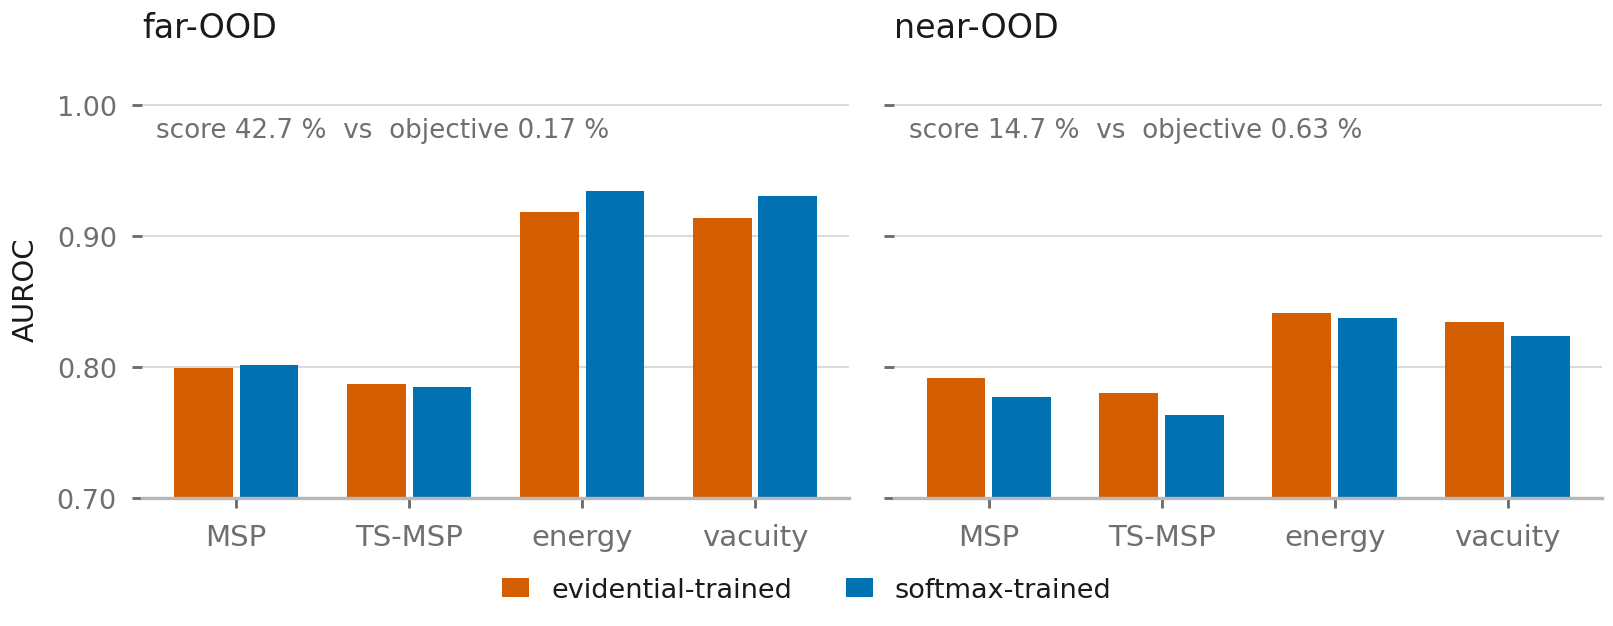
\includegraphics[width=\textwidth]{figures/F12_ood_score_vs_objective.png}
    \caption{OOD AUROC by scoring rule, split by which objective trained the model, for far- and near-OOD pools. The same score gives nearly the same AUROC regardless of which objective produced the logits it scores; the gap between scores dwarfs the gap between objectives.}
    \label{fig:ood-score-vs-objective}
\end{figure}

that the scoring rule accounts for roughly two to three orders of magnitude more OOD-detection variance than the training objective does. \textbf{This thesis deliberately reports the $\eta^2$ shares themselves rather than their quotient.} An earlier version of this analysis, computed on 99 of the 120 checkpoints before the grid's three missing cells were filled in, reported this as a ``163$\times$'' ratio; completing the remaining 21 checkpoints left both shares essentially unchanged (far-OOD score share moved from 43.68\% to 42.69\%, objective share from 0.267\% to 0.170\%) but moved the \emph{quotient} from 163$\times$ to 250.5$\times$ purely because the objective's already-tiny denominator shrank slightly further. A ratio computed against a near-zero denominator is unstable by construction and is not a number this thesis is willing to stand behind; the $\eta^2$ shares in \autoref{tab:rq2-eta2} are the stable, load-bearing quantity, and ``two to three orders of magnitude'' is as precise a verbal summary as the shares support. Concretely, the energy score achieves 0.9185 mean AUROC on evidential-trained logits and 0.9342 on softmax-trained logits (far-OOD) — close performance from the \emph{same} score regardless of which objective produced the logits it is scoring, while MSP remains close to 0.80 under either objective (0.7993 evidential-trained, 0.8014 softmax-trained). \textbf{It is the scoring rule, not the training objective, that produces the OOD-detection benefit the evidential head appeared to offer above.}

This precise gap — objective and scoring rule confounded in standard evaluation practice — is explicitly named as an open limitation by \textcite{genc2026objectives}, whose own study nonetheless covers a different objective family (metric and ranking losses, no evidential objective) and no frozen-backbone or few-shot setting, making this thesis's cross-application onto Dirichlet-trained logits a genuine extension rather than a duplication. \textcite{krumpl2026onemodel} run a related, larger-scale training-method-by-scoring-method ANOVA the same year and must be cited alongside this result rather than allowed to surface as an unacknowledged precedent; and \textcite{hayta2026pluginlosses}'s theoretical result that softmax is a special case of an evidential classifier under a particular loss family independently \emph{pre-explains} why the training objective contributes so little variance here — a result this thesis cites proactively rather than leaving for a reader to raise. What remains, after both of these are accounted for, is the specific empirical finding that cross-applying the energy score to Dirichlet-trained logits produces near-equivalence to softmax-trained energy scores — an evidential-specific angle this thesis's literature review found no precedent for.

\section{RQ3: Adapter Architecture versus Parameter Budget}
\label{sec:results-rq3}

\autoref{tab:rq1-eta2} found the adapter axis explains only 0.63\% of ECE variance overall — a small \emph{total} contribution. RQ3 asks a different, more targeted question: \emph{conditional on directly comparing two adapters}, which property of the adapter predicts the winner? An axis can contribute little total variance while still exhibiting a highly consistent \emph{direction} once the comparison is made pairwise, and that is exactly the pattern found here.

\subsubsection{The 16-pair evidence}

Sixteen matched bottleneck-versus-LoRA comparisons (2 datasets $\times$ 2 shot regimes $\times$ 2 backbones $\times$ 2 head interpretations, head interpretation held fixed within each pair) give the summary in \autoref{tab:rq3-16pair}.

\begin{table}[H]
    \centering
    \small
    \begin{tabular}{>{\raggedright\arraybackslash}p{4.4cm} >{\centering\arraybackslash}p{3.4cm} >{\centering\arraybackslash}p{3.4cm}}
        \toprule
        Outcome & Winner is bottleneck architecture & Winner is larger-budget arm \\
        \midrule
        Accuracy & \textbf{16 / 16} & 8 / 16 \\
        OOD AUROC (near, native score) & \textbf{16 / 16} & 8 / 16 \\
        OOD AUROC (TinyImageNet near) & \textbf{16 / 16} & 8 / 16 \\
        OOD AUROC (SVHN far) & 11 / 16 & 7 / 16 \\
        ECE (pooled) & 8 / 16 & \textbf{16 / 16} \\
        \bottomrule
    \end{tabular}
    \caption{Summary of 16 matched bottleneck-versus-LoRA comparisons. Because the parameter-budget ordering reverses between backbones (\autoref{tab:param-reversal}), the ``8/16'' entries are arithmetically implied by the other column, not independent evidence.}
    \label{tab:rq3-16pair}
\end{table}

\begin{figure}[H]
    \centering
    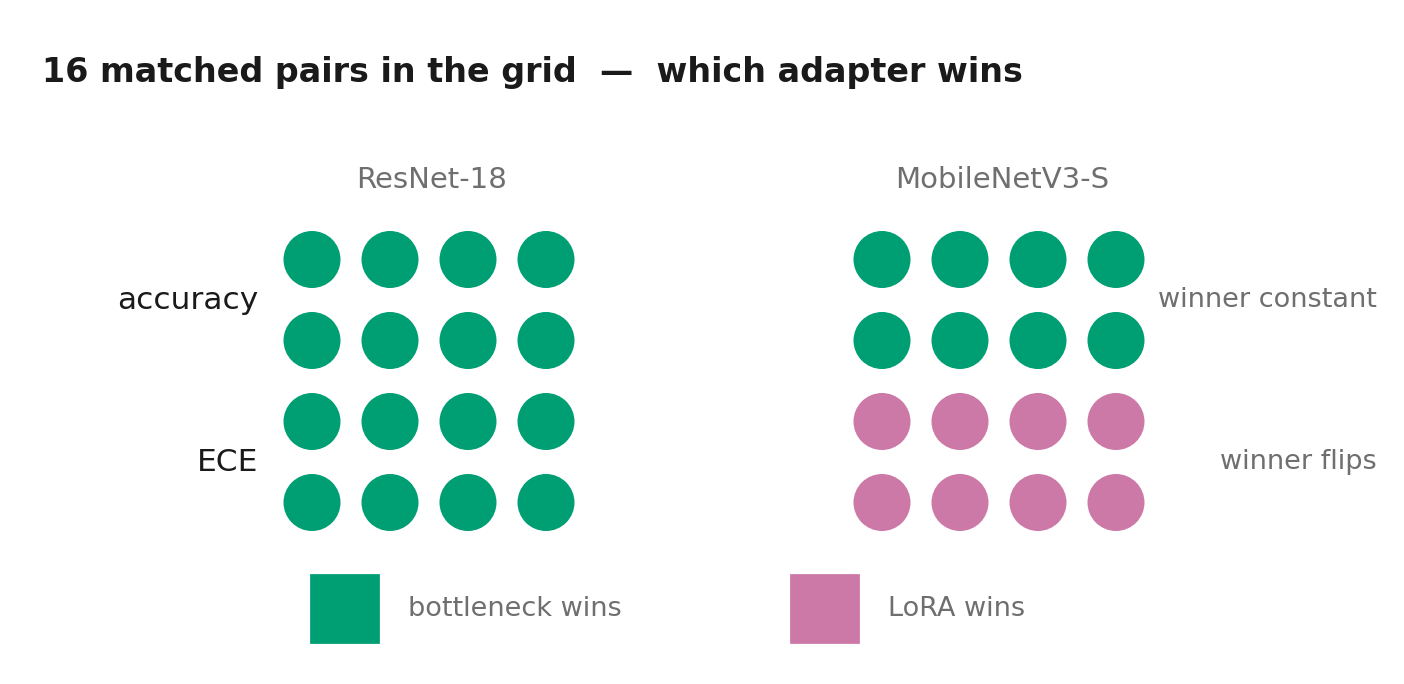
\includegraphics[width=0.85\textwidth]{figures/F13_matched_pairs_deltas.png}
    \caption{The 16 matched pairs: which adapter wins on accuracy and ECE, by backbone. The accuracy winner is constant (bottleneck); the ECE winner flips with the backbone.}
    \label{fig:matched-pairs-deltas}
\end{figure}

\begin{figure}[H]
    \centering
    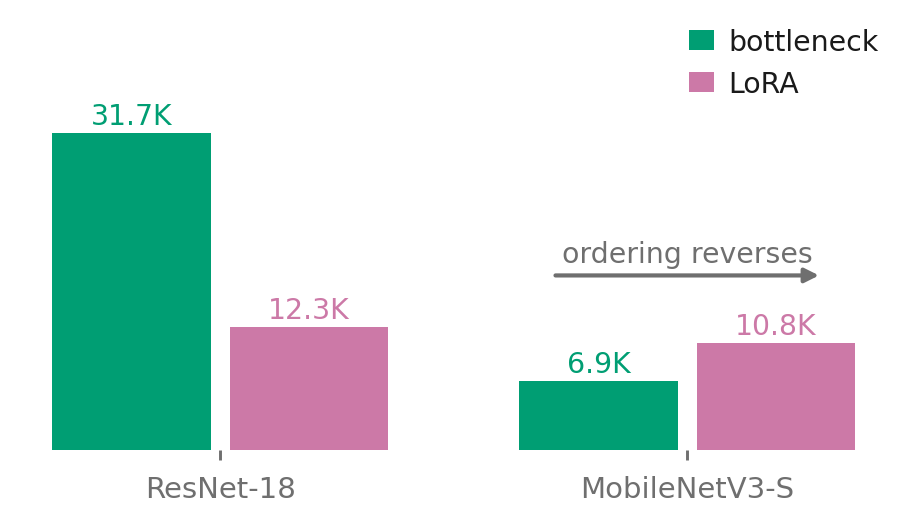
\includegraphics[width=0.7\textwidth]{figures/F5b_parameter_bars.png}
    \caption{The trainable-parameter-count reversal behind \autoref{tab:param-reversal}: bottleneck is the larger adapter on ResNet-18, LoRA is the larger adapter on MobileNetV3-Small.}
    \label{fig:parameter-bars-reversal}
\end{figure}

Because the budget ordering reverses exactly with the backbone (\autoref{tab:param-reversal}), any outcome perfectly consistent with architecture is \emph{necessarily} 8/16 on budget and vice versa, so the real content of \autoref{tab:rq3-16pair} is two directly observed facts, not the arithmetic 8/16 rows: (1) the accuracy winner does not change when the budget ordering reverses — bottleneck wins on both backbones despite holding 2.58$\times$ \emph{more} parameters on one and 1.55$\times$ \emph{fewer} on the other; and (2) the ECE winner \emph{does} change, exactly in step with the budget ordering — LoRA is better calibrated in all 8 MobileNetV3-Small pairs (where LoRA is larger) and bottleneck in all 8 ResNet-18 pairs (where bottleneck is larger). Each direction is a 16/16 sign-consistent result (two-sided $p \approx 3.05 \times 10^{-5}$ under a null of random direction), though the \emph{magnitude} of the ECE effect is weaker on CIFAR-FS: $|\Delta\mathrm{ECE}|$ exceeds twice the pooled across-seed standard deviation in only 2 of the 8 CIFAR-FS pairs, against all 8 of the MiniImageNet pairs.

On this evidence alone, ``calibration follows the larger parameter budget'' (hypothesis H3.2) and ``calibration follows some other, backbone-intrinsic property'' (hypothesis H3.2-alt) predict the \emph{identical} 16-pair pattern, because the two explanations are welded together by the accident of \autoref{tab:param-reversal}. The budget hypothesis is the more parsimonious reading of this data alone, but it is not \emph{established} by this data — it is merely not contradicted by it — which is precisely why the matched-budget follow-up experiment of \autoref{sec:method-matched-budget} was designed and run.

\subsubsection{The matched-budget adjudication}
\label{sec:results-matched-budget}

\autoref{tab:rq3-matched} reports the 48-run matched-budget experiment's per-cell calibration results, at residual parameter mismatch under 3.10\% (against 55--158\% in the unmatched 16-pair comparison above).

\begin{table}[H]
    \centering
    \footnotesize
    \begin{tabular}{>{\raggedright\arraybackslash}p{2.3cm} >{\raggedright\arraybackslash}p{1.6cm} >{\centering\arraybackslash}p{1.7cm} >{\centering\arraybackslash}p{1.5cm} >{\centering\arraybackslash}p{1.7cm} >{\raggedright\arraybackslash}p{2.6cm}}
        \toprule
        Backbone & Head & ECE (Bottl.) & ECE (LoRA) & $\Delta$ECE (LoRA $-$ Btl.) & Beyond 2$\sigma$? \\
        \midrule
        ResNet-18 & Evidential & \textbf{0.2955} & 0.4079 & $+0.112$ & Yes (both levels) \\
        ResNet-18 & Softmax & \textbf{0.0839} & 0.1829 & $+0.099$ & Yes (both levels) \\
        MobileNetV3-S & Evidential & 0.3171 & \textbf{0.3109} & $-0.006$ & Mostly yes (small effect) \\
        MobileNetV3-S & Softmax & 0.1122 & \textbf{0.1062} & $-0.006$ & Mixed (1 of 2 levels) \\
        \bottomrule
    \end{tabular}
    \caption{Matched-budget calibration results (averaged over the two pre-registered budget levels per backbone $\times$ head cell). Full per-level numbers are in \autoref{apx:results}.}
    \label{tab:rq3-matched}
\end{table}

\begin{figure}[H]
    \centering
    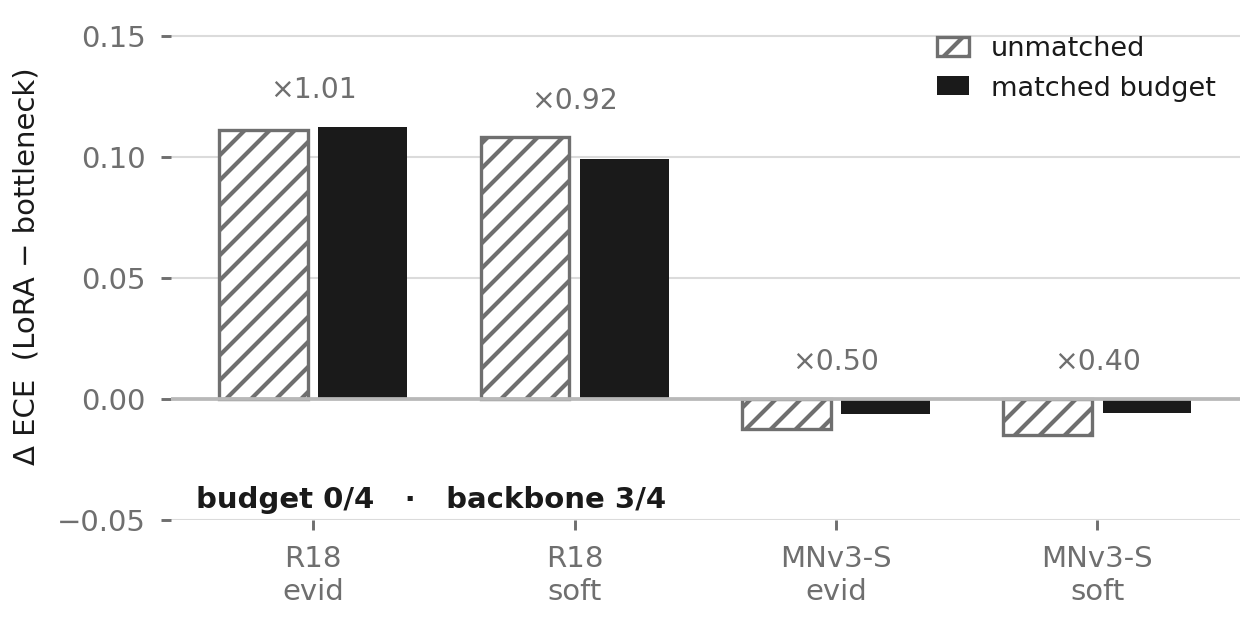
\includegraphics[width=0.85\textwidth]{figures/F14a_matched_budget_bars.png}
    \caption{$\Delta$ECE (LoRA $-$ bottleneck), unmatched versus matched budget, by backbone and head. The gap stays intact on ResNet-18 and roughly halves on MobileNetV3-Small — the backbone determines the sign, the budget only modulates the magnitude.}
    \label{fig:matched-budget-bars}
\end{figure}

\begin{figure}[H]
    \centering
    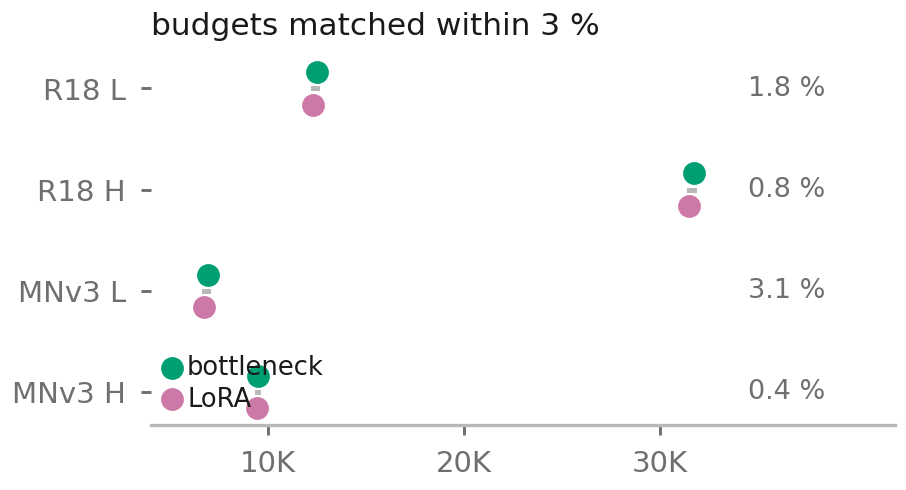
\includegraphics[width=0.6\textwidth]{figures/F8a_budget_match_inset.png}
    \caption{Residual parameter-count mismatch for each matched-budget pair, all under 3.1\% — the matched arms are close enough in size that the budget confound of \autoref{tab:param-reversal} genuinely no longer applies.}
    \label{fig:budget-match-inset}
\end{figure}

The pre-registered decision rule fires for \textbf{backbone-intrinsic} (H3.2-alt) in 3 of the 4 backbone-by-head cells, and for the budget hypothesis (H3.2) in \textbf{0 of 4}. On ResNet-18, equalising the adapters' parameter budgets leaves the calibration gap \emph{fully intact} — if anything slightly larger than in the unmatched comparison (collapse ratios of 1.01 and 0.92, i.e.\ the matched gap is as large as, or larger than, the original) — which is the opposite of what should happen if the budget difference were the actual cause. On MobileNetV3-Small, the matched gaps shrink to roughly half the unmatched ones (collapse ratios of 0.50 and 0.61), so budget is not entirely \emph{irrelevant} either — the honest reading is that \textbf{budget modulates the magnitude of the calibration gap, while the backbone determines its sign}. The two backbones' matched effect sizes are also wildly asymmetric and must not be presented as symmetric halves of one phenomenon: ResNet-18's matched $|\Delta\mathrm{ECE}|$ is on the order of 0.10--0.12, while MobileNetV3-Small's is on the order of 0.006 — an order of magnitude smaller.

Crucially, the accuracy half of RQ3's dissociation was genuinely at risk in this experiment and did not collapse: at matched budget, bottleneck wins accuracy and near-OOD AUROC in \textbf{8 of 8} cells, beyond 2$\sigma$ in all 8, with no cell's gap shrinking by more than about 40\% relative to the unmatched comparison. \textbf{RQ3's answer, restated to what the matched-budget experiment actually supports:} accuracy and near-OOD ranking follow adapter \emph{architecture}, invariant to which arm holds the larger parameter budget; calibration follows \emph{neither} architecture nor budget cleanly — it follows the \emph{backbone}, by a mechanism this two-backbone design cannot identify (\autoref{sec:results-limitations}). \textbf{The earlier reading, ``calibration follows the larger parameter budget,'' is superseded by this result and must not be presented as this thesis's finding.}

This finding appears to be genuinely novel: the standard convention in the NLP-PEFT literature is to \emph{equalise} budgets specifically to make comparisons fair, never to deliberately exploit a reversed budget ordering the way the base grid's structural accident permits, and no comparable architecture-versus-budget dissociation, adjudicated by a matched-budget design, was found in either the vision or NLP PEFT literature reviewed for this thesis. A same-family-named paper, \textcite{pandey2024bayesianpeft}, was checked specifically because of its similar name and confirmed to study a materially different question (ViT foundation models, no architecture-versus-budget dissociation) and is cited here as an explicit differentiation rather than left for a reader to conflate with this result.

\subsubsection{A demoted hypothesis: the interior-optimum budget curve}
\label{sec:results-rq5-demoted}

An earlier four-point curve across heterogeneous adapter types (Linear-Probe $\to$ LoRA $\to$ Bottleneck $\to$ Full-Fine-Tuning on CIFAR-FS/ResNet-18) appeared to show ECE falling then rising as trainable-parameter count increased, suggesting an interior calibration optimum distinct from the accuracy optimum. This comparison confounds parameter budget with adapter \emph{type} and with \emph{which} weights are trainable at all, so a controlled rank sweep was run instead — bottleneck architecture, backbone, dataset, and shot count all held fixed, only the bottleneck's internal rank varied across $\{1, 2, 4, 8, 16, 32, 64\}$ at 3 seeds each (21 runs). The interior optimum did \textbf{not} survive this controlled test: evidential ECE is lowest at the smallest rank tested (rank 1, ECE 0.291) and drifts noisily upward through rank 64 (ECE 0.309); the softmax curve moves in the \emph{opposite} direction, from 0.093 at rank 1 down to 0.081 at rank 64. The accuracy/calibration budget mismatch survives (the best-ECE rank and the best-accuracy rank differ) but via two roughly monotonic, oppositely-signed trends rather than a genuine U-shape, and — given that 3 seeds across 7 ranks is plausibly underpowered to rule out a subtle U-shape entirely — this thesis states the finding as \emph{``no interior optimum observed in the tested range''} rather than the stronger and less defensible \emph{``no interior optimum exists.''} One partial contradiction from the literature requires an explicit response: \textcite{muhlematter2026loraensemble} (LoRA-Ensemble), verified directly from its appendix figures, reports calibration \emph{degrading} at rank 32 for a Vision-Transformer, self-attention-based LoRA ensemble on CIFAR-100 — the same dataset family as CIFAR-FS, and a reversal this thesis's own softmax-head rank curve does not reproduce anywhere in the overlapping range. Three factors plausibly explain the discrepancy without dismissing it: LoRA-Ensemble adapts self-attention projections in a transformer rather than $1{\times}1$ convolutions in a CNN; it uses a trainable linear head over 100 classes rather than a parameter-free, similarity-bounded prototype head; and its tested rank range represents a far larger fraction of the backbone's own capacity than rank 64 does here (approximately 0.56\% of the frozen ResNet-18's parameters). This finding is retained in the thesis as a corrected negative result, not deleted, because it is itself informative: it retroactively supports RQ3's conclusion that architecture, not raw parameter count, is the more reliable causal lever for understanding these systems' calibration behaviour.

\section{RQ4: Post-Hoc Remediation of the Calibration Deficit}
\label{sec:results-rq4}

Refitting only the two evidence-affine parameters ($\mathrm{scale}$, $\mathrm{bias}$ in \autoref{eq:evidence-affine}) on each configuration's own held-out validation episodes, holding the adapter itself fixed at its already-trained weights, improves pooled ECE in \textbf{60 of 60 evidential cells (100\%)} across the full grid, by a mean absolute reduction of \textbf{0.139} (mean ECE falls from 0.323 to 0.185). Refit values cluster around $\mathrm{scale} \in [7, 14]$, well beyond the range the jointly-trained affine reaches on its own ($\mathrm{scale} \in [1.5, 4.5]$, \autoref{sec:method-recalibration}) — so the correct reading is that the operating point joint training converges to is far from the operating point that minimises validation ECE, not that a fixed default was poorly chosen.

\begin{figure}[H]
    \centering
    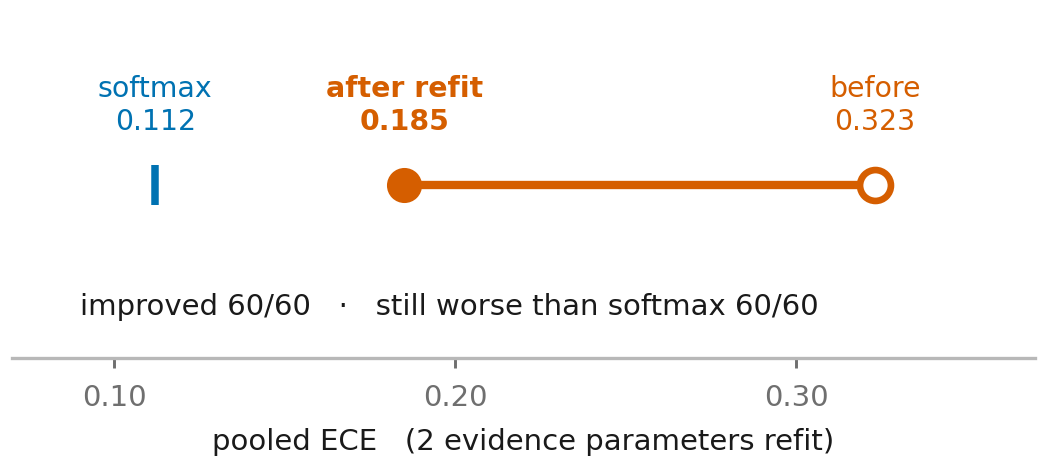
\includegraphics[width=0.75\textwidth]{figures/F15a_ece_before_after_dumbbell.png}
    \caption{Pooled ECE before and after the post-hoc refit, against the plain-softmax reference. The refit closes most, but not all, of the gap to softmax.}
    \label{fig:ece-before-after}
\end{figure}

\textbf{The refit narrows the calibration gap; it does not close it.} Even after refitting, the evidential head remains worse-calibrated than the plain softmax head in \textbf{60 of 60 cells} (mean 2.18$\times$ worse, best case 1.07$\times$, worst case 5.8$\times$) and worse than temperature-scaled softmax in \textbf{60 of 60 cells} (mean 13.6$\times$ worse). An earlier draft of this section reported only the improvement and not this comparison, which risks leaving the impression that post-hoc refitting closes the gap identified for RQ1 (\autoref{sec:results-rq1}); it does not, and both halves of the result are reported together here for that reason.

Because vacuity ($u = K/S$) is a function of \emph{all} $K$ logits jointly rather than a per-logit monotone transform, ranking preservation under this refit is not a guaranteed analytic consequence and was measured directly: OOD AUROC changes by no more than a small tolerance in \textbf{192 of 240 comparisons (80\%)}, with a mean AUROC change of essentially zero. Reordering does occur — the worst-case pool-and-cell combination shows a Spearman rank correlation of only 0.866 between the pre- and post-refit vacuity orderings, confirming the affine transform is not automatically rank-preserving for a sum-of-logits quantity like vacuity, exactly as the theoretical argument in \autoref{sec:method-recalibration} anticipated — but even that worst case remains a high, not a collapsed, correlation. In the remaining 20\% of comparisons, AUROC drops by more than the pre-specified tolerance; this thesis states the honest version of the claim, \emph{``the OOD ranking survives in the large majority of cases, with a measured minority exception,''} rather than the stronger and unsupported \emph{``ranking always survives.''}

\begin{figure}[H]
    \centering
    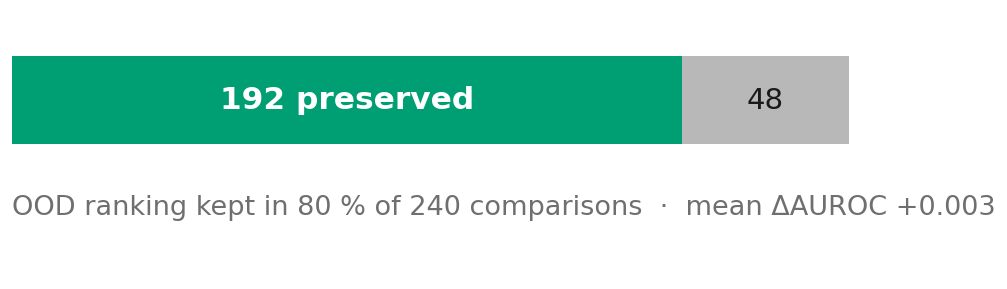
\includegraphics[width=0.75\textwidth]{figures/F15b_delta_auroc_strip.png}
    \caption{Change in OOD AUROC after the post-hoc refit, per pool and cell. Most changes cluster near zero; the minority exception is visible as the scattered points furthest from it.}
    \label{fig:delta-auroc-strip}
\end{figure}

This is deliberately the narrowest of the four research questions, and its scope must not be overstated. Post-hoc calibration itself is a mature field — Dirichlet calibration~\cite{kull2019dirichlet} (a differently-scoped use of the same word, \autoref{sec:related-calibration}) and invertible-logit post-hoc calibration~\cite{zhao2026invertible} both already exist for softmax-style classifiers. The magnitude of the ECE improvement found here is also not, on its own, remarkable: \textcite{guo2017calibration} report comparably large or larger temperature-scaling drops, and \textcite{linghu2022bel} (BEL), a directly analogous few-shot evidential system, reports drops of a similar order. The claim this thesis makes is therefore precisely scoped: a two-parameter post-hoc recalibration specifically for an \emph{evidential prototype head} in a frozen-backbone, few-shot regime, with OOD-ranking preservation \emph{measured} across 60 cells and 240 comparisons rather than assumed from the transform's algebraic form, and with the residual gap to softmax reported rather than left implicit — a systematic quantification this thesis's literature review found no precedent for, even though the general idea of post-hoc recalibration is well established.

\section{Implications: Deployment Cost}
\label{sec:results-implications}

Efficiency measurements across the twelve grid configurations profiled, plus real (untrained) reference measurements for ViT-B/16 and DeiT-Tiny, show that \textbf{backbone choice}, not adapter choice, is what drives inference latency: ResNet-18 is 5.12$\times$ slower than MobileNetV3-Small at matched adapter and head configuration, while switching adapter type changes latency by only 3.9--5.8\%. The evidential head's uncertainty computation is effectively free at inference: the mean absolute latency difference between evidential and softmax heads at matched backbone and adapter is 1.29\%, below this measurement session's own 5.91\% noise floor, and the uncertainty-scoring step itself costs only 1.09\% of a single image's backbone forward-pass time for a 75-query episode — directly confirming, in this specific system, \textcite{sensoy2018edl}'s claim that evidential uncertainty is available at negligible extra inference cost compared to ensembling or Monte Carlo sampling.

\begin{table}[H]
    \centering
    \begin{tabular}{lr}
        \toprule
        Design choice & Effect on latency \\
        \midrule
        Backbone (ResNet-18 vs.\ MobileNetV3-Small) & \textbf{5.1$\times$} \\
        Adapter type & 4--6\% \\
        Evidential vs.\ softmax head & $\sim$1\%, within measurement noise \\
        \bottomrule
    \end{tabular}
    \caption{Measured effect of each design choice on inference latency. The backbone dominates; adapter choice matters far more for accuracy (\autoref{sec:results-rq3}) than for latency.}
    \label{tab:latency-effects}
\end{table}

\begin{figure}[H]
    \centering
    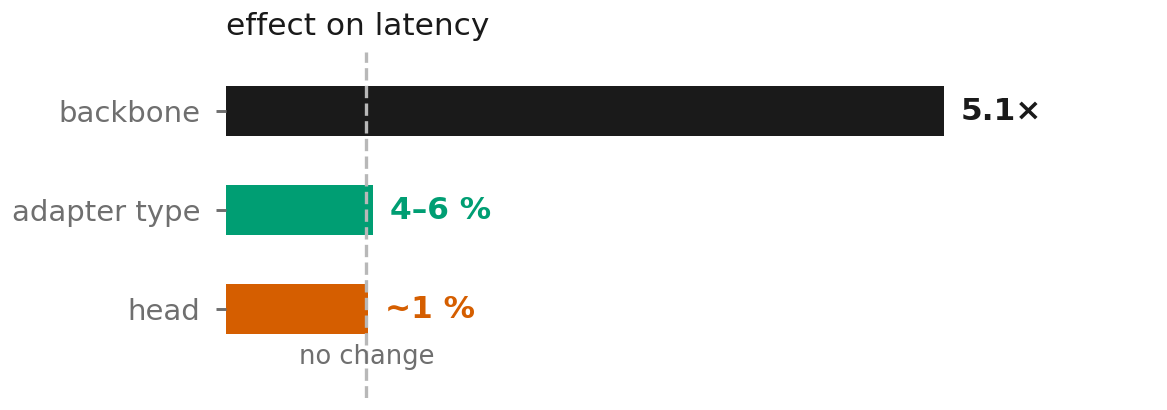
\includegraphics[width=0.75\textwidth]{figures/D3_latency_effect_bars.png}
    \caption{Effect on inference latency of backbone, adapter type, and head interpretation, measured on a canonical edge-proxy CPU session.}
    \label{fig:latency-effect-bars}
\end{figure}

The recommended edge-deployment point identified by this analysis is MobileNetV3-Small with a parallel-bottleneck adapter and an evidential head: 11.86\,ms inference latency at 6{,}930 trainable parameters, combining the smallest backbone, a near-Pareto-optimal adapter (\autoref{sec:results-param-efficiency}), and an uncertainty mechanism that costs essentially nothing at inference despite its calibration cost at training time (\autoref{sec:results-rq1}).

\section{Positioning Against the State of the Art}
\label{sec:results-positioning}

Because this thesis's absolute accuracy numbers rest on a frozen ImageNet-pretrained backbone while the standard few-shot literature trains its backbone from scratch on the base classes, and because MiniImageNet's classes are themselves a subset of ImageNet, the comparisons in this section are read as a controlled study of \emph{parameter efficiency at fixed protocol}, not a claim of new state-of-the-art accuracy (\autoref{sec:results-limitations} states this caveat again explicitly, as it must be kept in view throughout this section).

\begin{table}[H]
    \centering
    \footnotesize
    \begin{tabular}{>{\raggedright\arraybackslash}p{4cm} >{\raggedright\arraybackslash}p{2.3cm} >{\raggedright\arraybackslash}p{1.7cm} r r}
        \toprule
        Method & Backbone & Trainable params & CIFAR-FS 5-shot & MiniImageNet 5-shot \\
        \midrule
        Sup-21k$\to$ProtoNet~\cite{hu2022pmf} & ViT-B/16 & $\sim$85.8\,M & 96.7 & 99.2 \\
        DINO$\to$ProtoNet~\cite{caron2021dino,hu2022pmf} & ViT-B/16 & $\sim$85.8\,M & 92.2 & 98.4 \\
        DINO$\to$ProtoNet~\cite{caron2021dino,hu2022pmf} & ViT-S/16 & $\sim$21\,M & 92.5 & 98.0 \\
        DINO$\to$ProtoNet~\cite{caron2021dino,hu2022pmf} & ResNet-50 & $\sim$25\,M & --- & 92.0 \\
        BEL~\cite{linghu2022bel} & ResNet-12 & not reported & 86.92 & 79.60 \\
        MetaOptNet (from scratch)~\cite{lee2019metaoptnet} & ResNet-12 & not reported & 84.2 & 78.63 \\
        \textbf{B-PEFT (ours)}, parallel bottleneck & \textbf{ResNet-18, frozen} & \textbf{31{,}744} & \textbf{91.44} & \textbf{95.56} \\
        \textbf{B-PEFT (ours)}, parallel bottleneck & \textbf{MobileNetV3-S, frozen} & \textbf{6{,}928} & \textbf{90.74} & 90.10 \\
        \bottomrule
    \end{tabular}
    \caption{Accuracy versus trainable-parameter budget on the same 5-way 5-shot episodic protocol. No competing method in this table reports macro-F1, calibration, or OOD detection.}
    \label{tab:positioning-accuracy}
\end{table}

Three conclusions follow from \autoref{tab:positioning-accuracy}, kept deliberately separate rather than blurred into one headline number. First, at 5-shot on CIFAR-FS the parameter saving is close to free: this thesis's 31{,}744-parameter ResNet-18 adapter is 1.06 percentage points behind a fully meta-trained DINO ViT-S while training 662$\times$ fewer parameters, and 0.76 points behind ViT-B at 2{,}703$\times$ fewer. Second, backbone-family-matched, this thesis's system simply wins: against DINO$\to$ProtoNet on a ResNet-50 backbone, this thesis's adapter is 3.56 and 5.83 percentage points \emph{ahead} on MiniImageNet 5-shot and 1-shot respectively, at 788$\times$ fewer trainable parameters — indicating that the residual gap to the strongest published numbers is a Vision-Transformer gap, not a parameter-efficiency gap. Third, the trade is genuinely unfavourable at 1-shot and on MiniImageNet with the smaller backbone, by as much as 18 percentage points against the strongest ViT baselines; this thesis volunteers this rather than reporting only the favourable comparisons, because MiniImageNet's classes are themselves drawn from ImageNet, so a larger pretrained representation carries proportionally more of the answer there than on CIFAR-FS.

On the deployment side, this thesis's system trains 6{,}928 to 31{,}744 parameters against 240{,}000 to 85{,}840{,}000 for standard Vision-Transformer PEFT methods on the unrelated VTAB-1k protocol~\cite{lian2022ssf,jia2022vpt,zhou2022coop} — a difference of one to four orders of magnitude — and its 2.5-million-parameter MobileNetV3-Small backbone is 34.6$\times$ smaller at inference than a CLIP ViT-B/16 backbone, which itself cannot fit within the 32--512\,kB SRAM and sub-1\,MB flash budgets typical of microcontroller-class edge hardware~\cite{somvanshi2025tinydl} under any quantisation scheme. This is the deployment case this thesis's choice of frozen, lightweight CNN backbones is built to support, and it is not disputed that a sufficiently large Vision Transformer remains the stronger backbone where its resource footprint is affordable~\cite{simeoni2025dinov3}.

\section{Threats to Validity and Limitations}
\label{sec:results-limitations}

Five limitations apply across every result in this chapter and are stated here rather than left implicit.

\begin{enumerate}
    \item \textbf{ImageNet-pretraining overlap.} Both backbones are ImageNet-pretrained, while the standard CIFAR-FS/MiniImageNet protocol assumes training from scratch on the base classes; MiniImageNet's ``novel'' test classes were, in fact, seen during ImageNet pretraining. This means the absolute accuracies reported in \autoref{sec:results-positioning} are not directly comparable to from-scratch few-shot literature. The research questions of \autoref{sec:intro-rqs} concern \emph{relative} differences between design choices under a fixed backbone, which mitigates but does not eliminate this caveat.
    \item \textbf{One frozen hyperparameter recipe.} All 40 grid configurations share a single hyperparameter recipe, tuned once rather than re-tuned per cell. The grid therefore answers ``how do these design axes compare under one fixed recipe,'' not ``what is the best achievable number for each individual cell.''
    \item \textbf{Three training seeds, and effectively one for two baselines.} Full-Fine-Tuning and Linear-Probe have zero across-seed variance by construction (\autoref{sec:method-implementation}), so any claim resting on a small margin over either baseline should be read with $n=1$ effective seeds for that comparison, not $n=3$.
    \item \textbf{The mechanism behind RQ3's backbone-intrinsic finding is not identified.} ``Backbone-intrinsic'' (\autoref{sec:results-matched-budget}) describes where the matched-budget evidence points, not an explanation of \emph{why}: depth, width, normalisation scheme, the inverted-residual block structure specific to MobileNetV3, and feature-norm scale at the adapter insertion sites are all plausible candidate mechanisms, and two backbones cannot separate them. This is stated as an open question for future work (\autoref{chapter:conclusion}) rather than resolved with a plausible-sounding but untested narrative.
    \item \textbf{Novelty claims rest on a non-exhaustive literature search.} The positioning and novelty statements throughout \autoref{chapter:related-works} and this chapter reflect a systematic but necessarily incomplete literature review; absence of a found precedent is evidence of absence only to the extent the search was thorough, and is reported here as the best available evidence rather than a certainty.
\end{enumerate}


% =======================================================================
\chapter{Conclusion}
\label{chapter:conclusion}
% =======================================================================

\section{Restating the Research Questions}

This thesis set out to answer four questions about which design choices govern which aspects of reliability in a parameter-efficient, few-shot vision system built on frozen, lightweight CNN backbones: which design choices most strongly explain variation in accuracy, calibration, and out-of-distribution detection (RQ1); whether out-of-distribution detection is explained more by the training objective or by the scoring rule (RQ2); whether accuracy follows adapter architecture and calibration follows parameter budget (RQ3); and whether evidential calibration can be repaired after training without breaking out-of-distribution detection (RQ4). These four questions supersede the original research proposal's four comparison-style questions (adapter placement, evidential-versus-softmax calibration, Bayesian near-OOD detection, and a latency Pareto frontier, \autoref{sec:intro-rqs}), three of which a literature audit found closely anticipated by prior work; every experiment behind those original questions is retained as evidence for whichever of RQ1--RQ4 it now supports. All four questions are answered in \autoref{chapter:results}, RQ3 adjudicated by a dedicated, pre-registered matched-budget experiment, and these four answers are what this thesis is ultimately judged on.

\section{Summary of Key Findings}

A single placement pilot ties on accuracy between serial and parallel bottleneck insertion but favours parallel on calibration and far-OOD detection, and a 31{,}744-parameter parallel-bottleneck adapter matches or beats full fine-tuning of an 11.18-million-parameter backbone at 0.28\% of its parameter cost. The evidential head is decisively worse-calibrated than softmax across every tested configuration — a clean, reproducible negative result consistent with independent theoretical work — while simultaneously being a substantially better OOD ranker than softmax-probability-based scores, though a training-free energy score generally beats it. Separating training objective from scoring rule shows the scoring rule, not the objective, accounts for roughly two to three orders of magnitude more of that OOD-detection benefit (42.69\% versus 0.17\% $\eta^2$ on far-OOD). Head interpretation governs roughly 83\% of calibration variance and under 0.2\% of accuracy variance, while shot count governs roughly three-quarters of accuracy variance — accuracy and calibration are controlled by almost entirely separate design axes. Within the adapter axis specifically, accuracy and near-OOD detection follow adapter \emph{architecture} regardless of which adapter holds the larger parameter budget, confirmed at matched budget in 8 of 8 cells; calibration, however, is governed by the \emph{backbone} rather than by either architecture or budget, a finding only a dedicated matched-budget experiment — not the base grid alone — could establish, and by a mechanism this two-backbone design leaves genuinely unidentified. Finally, the evidential head's calibration deficit can be meaningfully narrowed, at negligible additional parameter cost, by refitting only its two evidence-affine parameters after training — though even after refitting it remains worse-calibrated than softmax in every tested configuration — while its OOD ranking survives that refit in the large majority, though not all, of the configurations tested.

\begin{table}[H]
    \centering
    \small
    \begin{tabular}{l >{\raggedright\arraybackslash}p{3.4cm} >{\raggedright\arraybackslash}p{6.3cm}}
        \toprule
        Reliability aspect & Main factor & Evidence \\
        \midrule
        Accuracy & Shots + adapter architecture & 76\% of variation; bottleneck wins 8/8 at matched budget \\
        Calibration & Head + backbone & 83\% of variation; backbone dependence 3/4 cells, budget 0/4 \\
        OOD detection & Scoring rule & 42.7\% vs.\ 0.17\% of far-OOD variation (score vs.\ objective) \\
        Calibration repair & Post-hoc evidence refit & ECE improved 60/60; still worse than softmax 60/60 \\
        \bottomrule
    \end{tabular}
    \caption{What this thesis learned: no single design choice optimises every reliability axis.}
    \label{tab:conclusion-summary}
\end{table}

\begin{figure}[H]
    \centering
    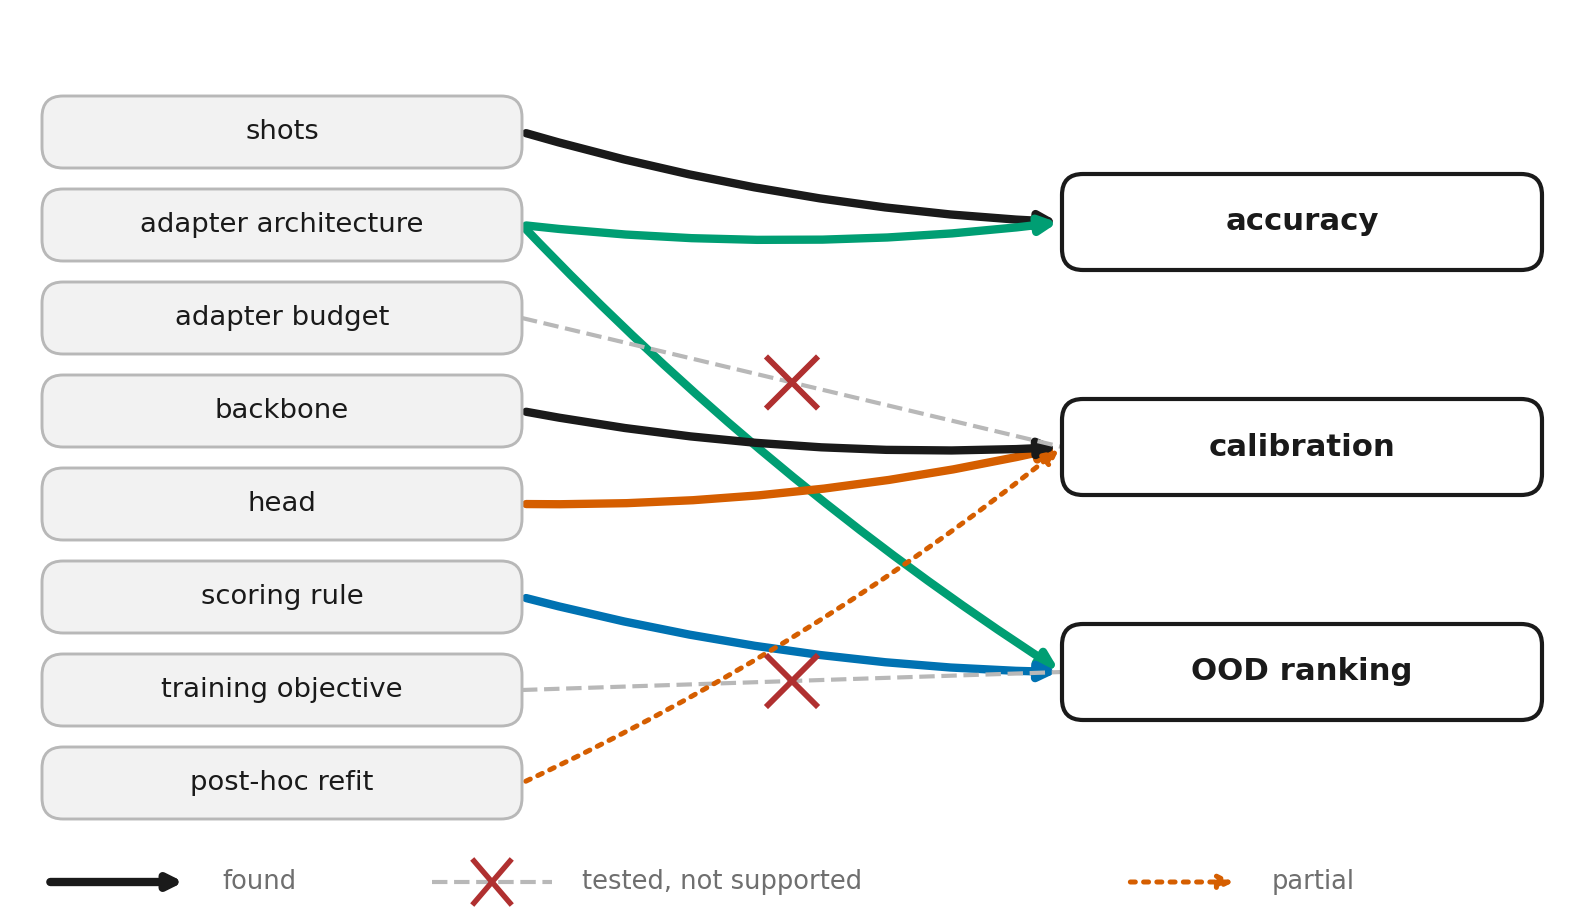
\includegraphics[width=0.85\textwidth]{figures/F16_findings_graph.png}
    \caption{Every design factor tested against every reliability outcome: which links were found, which were tested and not supported, and which are partial. Adapter budget alone does not reach calibration or OOD ranking; architecture and scoring rule do the work that a first look at parameter count alone would suggest budget was doing.}
    \label{fig:findings-graph}
\end{figure}

The main contribution of this thesis is not a universally superior model, but a controlled decomposition of which design choices govern which aspects of reliability in this few-shot PEFT regime.

\section{Contributions of the Research}

Beyond the specific findings above, this thesis contributes a reproducible, config-driven B-PEFT implementation; a balanced 120-run experimental grid permitting a formal variance decomposition that single-axis PEFT studies cannot compute; a pre-registered matched-budget experiment design, generally applicable beyond this thesis's specific adapters, for separating architecture from parameter budget in any PEFT comparison where the two happen to be confounded; and an explicit correction record for three claims (an early evidential-versus-energy parity result, an apparent interior-optimum calibration curve, and a mis-scoped external citation) that did not survive more rigorous later testing, reported alongside the evidence that overturned them rather than silently revised away.

\section{Limitations}

The five limitations of \autoref{sec:results-limitations} — ImageNet-pretraining overlap, a single frozen hyperparameter recipe, effectively single-seed baselines, an unidentified mechanism behind the backbone-intrinsic calibration finding, and a necessarily incomplete literature search — apply to every finding in this thesis and are not repeated in full here; the most consequential for future work is the second-to-last, addressed directly in the next section.

\section{Suggestions for Future Work}

Four directions follow directly from this thesis's own findings rather than from a generic wish list. First, and most directly motivated by \autoref{sec:results-limitations}'s fourth point, adding a third and fourth backbone family — varying depth, width, normalisation, and block structure independently rather than jointly, as ResNet-18 and MobileNetV3-Small currently do — would let a future study separate the specific structural property responsible for the backbone-intrinsic calibration effect this thesis identifies but cannot explain. Second, a Vision-Transformer arm (a ViT-Tiny or DeiT-Small backbone under this thesis's exact protocol) would convert \autoref{sec:results-positioning}'s literature-based accuracy comparison into a directly measured one, closing the single most exposed gap in this thesis's positioning argument. Third, a from-scratch (non-ImageNet-pretrained) backbone control run would directly quantify the pretraining-overlap confound rather than only bounding it qualitatively. Fourth, the two additional in-distribution datasets named in the original proposal but not run in this thesis's grid — CUB-200-2011 for fine-grained classification and a medical-imaging dataset such as ISIC — would test whether this thesis's attribution findings, established on natural-image benchmarks, generalise to domains where the visual features distinguishing classes are far more subtle.

\section{Concluding Remarks}

This thesis set out to ask whether a Bayesian uncertainty mechanism makes a parameter-efficiently adapted, lightweight CNN more reliable in the few-shot regime, and found an answer more nuanced than a simple yes or no: the evidential head this thesis studies is a worse-calibrated, but more discriminative, alternative to softmax, and that trade-off is governed by design axes — training objective versus scoring rule, adapter architecture versus parameter budget, a fixed default versus a post-hoc refit — that a single comparison-style research question cannot separate, but a balanced experimental grid and a purpose-built adjudicating experiment can. The final, defensible claims are narrower and more precisely scoped than the thesis's original proposal anticipated, and are reported here exactly as narrow as the evidence supports: not because the ambitious version would have been more satisfying to write, but because a thesis whose claims survive its own literature audit is worth more than one that does not.

%-------------------------- BACK MATTER --------------------------%

\printbib

\begin{appendices}

% =======================================================================
\chapter{Full Experimental Result Tables}
\label{apx:results}
% =======================================================================

This appendix reproduces, in full, the four core result tables selectively referenced throughout \autoref{chapter:results}: accuracy, macro-F1 and trainable-parameter count (\autoref{tab:apx-accuracy}); calibration (\autoref{tab:apx-calibration}); OOD-detection AUROC (\autoref{tab:apx-auroc}); and OOD FPR@95\%TPR (\autoref{tab:apx-fpr95}). All four are computed over the identical frozen 600-episode test stream (\autoref{sec:proto-episodic}), averaged over 3 training seeds (42, 43, 44) per configuration.

\begingroup
\footnotesize
\begin{longtable}{ll l >{\raggedright\arraybackslash}p{3.1cm} rrr}
\caption{Accuracy, macro-F1, and trainable parameters for all 40 grid configurations.}
\label{tab:apx-accuracy} \\
\toprule
Dataset & Shots & Backbone & Adapter/Head & Params & Accuracy \% & Macro-F1 \% \\
\midrule
\endfirsthead
\multicolumn{7}{c}{\tablename\ \thetable\ -- continued} \\
\toprule
Dataset & Shots & Backbone & Adapter/Head & Params & Accuracy \% & Macro-F1 \% \\
\midrule
\endhead
\midrule \multicolumn{7}{r}{continued on next page} \\
\endfoot
\bottomrule
\endlastfoot
CIFAR-FS & 1-shot & ResNet-18 & Bottleneck-par / Evid. & 31{,}746 & 79.19 & 78.29 \\
CIFAR-FS & 1-shot & ResNet-18 & Bottleneck-par / Softmax & 31{,}744 & 78.57 & 77.50 \\
CIFAR-FS & 1-shot & ResNet-18 & LoRA / Evid. & 12{,}290 & 73.76 & 72.61 \\
CIFAR-FS & 1-shot & ResNet-18 & LoRA / Softmax & 12{,}288 & 75.44 & 74.33 \\
CIFAR-FS & 1-shot & ResNet-18 & Full-FT* / Evid. & 11{,}176{,}514 & 80.36 & 79.14 \\
CIFAR-FS & 1-shot & ResNet-18 & Full-FT* / Softmax & 11{,}176{,}512 & 81.14 & 80.02 \\
CIFAR-FS & 1-shot & ResNet-18 & Linear-Probe* / Evid. & 2 & 70.25 & 69.10 \\
CIFAR-FS & 1-shot & ResNet-18 & Linear-Probe* / Softmax & 0 & 70.25 & 69.10 \\
CIFAR-FS & 1-shot & MobileNetV3-S & Bottleneck-par / Evid. & 6{,}930 & 78.88 & 77.83 \\
CIFAR-FS & 1-shot & MobileNetV3-S & Bottleneck-par / Softmax & 6{,}928 & 78.80 & 77.69 \\
CIFAR-FS & 1-shot & MobileNetV3-S & LoRA / Evid. & 10{,}754 & 74.03 & 72.47 \\
CIFAR-FS & 1-shot & MobileNetV3-S & LoRA / Softmax & 10{,}752 & 75.43 & 74.09 \\
CIFAR-FS & 5-shot & ResNet-18 & Bottleneck-par / Evid. & 31{,}746 & 91.58 & 91.46 \\
CIFAR-FS & 5-shot & ResNet-18 & Bottleneck-par / Softmax & 31{,}744 & 91.44 & 91.29 \\
CIFAR-FS & 5-shot & ResNet-18 & LoRA / Evid. & 12{,}290 & 83.33 & 82.96 \\
CIFAR-FS & 5-shot & ResNet-18 & LoRA / Softmax & 12{,}288 & 86.25 & 85.98 \\
CIFAR-FS & 5-shot & ResNet-18 & Full-FT* / Evid. & 11{,}176{,}514 & 88.82 & 88.56 \\
CIFAR-FS & 5-shot & ResNet-18 & Full-FT* / Softmax & 11{,}176{,}512 & 90.47 & 90.27 \\
CIFAR-FS & 5-shot & ResNet-18 & Linear-Probe* / Evid. & 2 & 87.41 & 87.28 \\
CIFAR-FS & 5-shot & ResNet-18 & Linear-Probe* / Softmax & 0 & 87.41 & 87.28 \\
CIFAR-FS & 5-shot & MobileNetV3-S & Bottleneck-par / Evid. & 6{,}930 & 90.24 & 90.08 \\
CIFAR-FS & 5-shot & MobileNetV3-S & Bottleneck-par / Softmax & 6{,}928 & 90.74 & 90.59 \\
CIFAR-FS & 5-shot & MobileNetV3-S & LoRA / Evid. & 10{,}754 & 86.97 & 86.73 \\
CIFAR-FS & 5-shot & MobileNetV3-S & LoRA / Softmax & 10{,}752 & 88.05 & 87.79 \\
MiniImageNet & 1-shot & ResNet-18 & Bottleneck-par / Evid. & 31{,}746 & 84.81 & 84.21 \\
MiniImageNet & 1-shot & ResNet-18 & Bottleneck-par / Softmax & 31{,}744 & 85.03 & 84.34 \\
MiniImageNet & 1-shot & ResNet-18 & LoRA / Evid. & 12{,}290 & 79.16 & 78.11 \\
MiniImageNet & 1-shot & ResNet-18 & LoRA / Softmax & 12{,}288 & 80.29 & 79.36 \\
MiniImageNet & 1-shot & MobileNetV3-S & Bottleneck-par / Evid. & 6{,}930 & 75.61 & 74.53 \\
MiniImageNet & 1-shot & MobileNetV3-S & Bottleneck-par / Softmax & 6{,}928 & 74.92 & 73.71 \\
MiniImageNet & 1-shot & MobileNetV3-S & LoRA / Evid. & 10{,}754 & 72.48 & 70.97 \\
MiniImageNet & 1-shot & MobileNetV3-S & LoRA / Softmax & 10{,}752 & 72.45 & 70.98 \\
MiniImageNet & 5-shot & ResNet-18 & Bottleneck-par / Evid. & 31{,}746 & 95.88 & 95.85 \\
MiniImageNet & 5-shot & ResNet-18 & Bottleneck-par / Softmax & 31{,}744 & 95.56 & 95.53 \\
MiniImageNet & 5-shot & ResNet-18 & LoRA / Evid. & 12{,}290 & 88.32 & 88.20 \\
MiniImageNet & 5-shot & ResNet-18 & LoRA / Softmax & 12{,}288 & 91.56 & 91.48 \\
MiniImageNet & 5-shot & MobileNetV3-S & Bottleneck-par / Evid. & 6{,}930 & 90.64 & 90.55 \\
MiniImageNet & 5-shot & MobileNetV3-S & Bottleneck-par / Softmax & 6{,}928 & 90.10 & 89.97 \\
MiniImageNet & 5-shot & MobileNetV3-S & LoRA / Evid. & 10{,}754 & 87.96 & 87.79 \\
MiniImageNet & 5-shot & MobileNetV3-S & LoRA / Softmax & 10{,}752 & 87.96 & 87.82 \\
\end{longtable}
\endgroup

\begingroup
\footnotesize
\begin{longtable}{ll >{\raggedright\arraybackslash}p{4.6cm} rrr}
\caption{Calibration (pooled ECE, per-episode ECE, Brier score) for all 40 grid configurations. ECE after temperature scaling applies to softmax cells only.}
\label{tab:apx-calibration} \\
\toprule
Dataset & Shots & Backbone / Adapter / Head & ECE (pooled) & ECE (per-ep.) & Brier \\
\midrule
\endfirsthead
\multicolumn{6}{c}{\tablename\ \thetable\ -- continued} \\
\toprule
Dataset & Shots & Backbone / Adapter / Head & ECE (pooled) & ECE (per-ep.) & Brier \\
\midrule
\endhead
\midrule \multicolumn{6}{r}{continued on next page} \\
\endfoot
\bottomrule
\endlastfoot
CIFAR-FS & 1-shot & ResNet-18 / Bottleneck-par / Evid. & 0.2765 & 0.2885 & 0.4050 \\
CIFAR-FS & 1-shot & ResNet-18 / Bottleneck-par / Softmax & 0.0560 & 0.1364 & 0.3084 \\
CIFAR-FS & 1-shot & ResNet-18 / LoRA / Evid. & 0.2970 & 0.3096 & 0.4959 \\
CIFAR-FS & 1-shot & ResNet-18 / LoRA / Softmax & 0.0969 & 0.1592 & 0.3579 \\
CIFAR-FS & 1-shot & ResNet-18 / Full-FT* / Evid. & 0.3207 & 0.3290 & 0.4254 \\
CIFAR-FS & 1-shot & ResNet-18 / Full-FT* / Softmax & 0.0854 & 0.1468 & 0.2850 \\
CIFAR-FS & 1-shot & ResNet-18 / Linear-Probe* / Evid. & 0.4397 & 0.4397 & 0.7038 \\
CIFAR-FS & 1-shot & ResNet-18 / Linear-Probe* / Softmax & 0.2818 & 0.2944 & 0.5283 \\
CIFAR-FS & 1-shot & MobileNetV3-S / Bottleneck-par / Evid. & 0.2540 & 0.2702 & 0.3973 \\
CIFAR-FS & 1-shot & MobileNetV3-S / Bottleneck-par / Softmax & 0.0499 & 0.1347 & 0.3070 \\
CIFAR-FS & 1-shot & MobileNetV3-S / LoRA / Evid. & 0.2156 & 0.2423 & 0.4361 \\
CIFAR-FS & 1-shot & MobileNetV3-S / LoRA / Softmax & 0.0287 & 0.1357 & 0.3461 \\
CIFAR-FS & 5-shot & ResNet-18 / Bottleneck-par / Evid. & 0.3010 & 0.3070 & 0.2513 \\
CIFAR-FS & 5-shot & ResNet-18 / Bottleneck-par / Softmax & 0.0670 & 0.0989 & 0.1332 \\
CIFAR-FS & 5-shot & ResNet-18 / LoRA / Evid. & 0.3294 & 0.3366 & 0.3888 \\
CIFAR-FS & 5-shot & ResNet-18 / LoRA / Softmax & 0.1016 & 0.1353 & 0.2156 \\
CIFAR-FS & 5-shot & ResNet-18 / Full-FT* / Evid. & 0.3383 & 0.3423 & 0.3220 \\
CIFAR-FS & 5-shot & ResNet-18 / Full-FT* / Softmax & 0.0728 & 0.1048 & 0.1536 \\
CIFAR-FS & 5-shot & ResNet-18 / Linear-Probe* / Evid. & 0.6234 & 0.6234 & 0.7078 \\
CIFAR-FS & 5-shot & ResNet-18 / Linear-Probe* / Softmax & 0.4476 & 0.4516 & 0.4554 \\
CIFAR-FS & 5-shot & MobileNetV3-S / Bottleneck-par / Evid. & 0.3043 & 0.3117 & 0.2708 \\
CIFAR-FS & 5-shot & MobileNetV3-S / Bottleneck-par / Softmax & 0.0703 & 0.1039 & 0.1464 \\
CIFAR-FS & 5-shot & MobileNetV3-S / LoRA / Evid. & 0.2879 & 0.2993 & 0.2991 \\
CIFAR-FS & 5-shot & MobileNetV3-S / LoRA / Softmax & 0.0616 & 0.1065 & 0.1793 \\
MiniImageNet & 1-shot & ResNet-18 / Bottleneck-par / Evid. & 0.3073 & 0.3158 & 0.3523 \\
MiniImageNet & 1-shot & ResNet-18 / Bottleneck-par / Softmax & 0.1012 & 0.1416 & 0.2352 \\
MiniImageNet & 1-shot & ResNet-18 / LoRA / Evid. & 0.3708 & 0.3785 & 0.4909 \\
MiniImageNet & 1-shot & ResNet-18 / LoRA / Softmax & 0.1748 & 0.2035 & 0.3282 \\
MiniImageNet & 1-shot & MobileNetV3-S / Bottleneck-par / Evid. & 0.2534 & 0.2664 & 0.4402 \\
MiniImageNet & 1-shot & MobileNetV3-S / Bottleneck-par / Softmax & 0.0650 & 0.1433 & 0.3551 \\
MiniImageNet & 1-shot & MobileNetV3-S / LoRA / Evid. & 0.2194 & 0.2417 & 0.4557 \\
MiniImageNet & 1-shot & MobileNetV3-S / LoRA / Softmax & 0.0242 & 0.1368 & 0.3796 \\
MiniImageNet & 5-shot & ResNet-18 / Bottleneck-par / Evid. & 0.2938 & 0.2993 & 0.1883 \\
MiniImageNet & 5-shot & ResNet-18 / Bottleneck-par / Softmax & 0.0850 & 0.1014 & 0.0856 \\
MiniImageNet & 5-shot & ResNet-18 / LoRA / Evid. & 0.4049 & 0.4093 & 0.3977 \\
MiniImageNet & 5-shot & ResNet-18 / LoRA / Softmax & 0.1930 & 0.2063 & 0.1913 \\
MiniImageNet & 5-shot & MobileNetV3-S / Bottleneck-par / Evid. & 0.3177 & 0.3229 & 0.2817 \\
MiniImageNet & 5-shot & MobileNetV3-S / Bottleneck-par / Softmax & 0.1107 & 0.1339 & 0.1699 \\
MiniImageNet & 5-shot & MobileNetV3-S / LoRA / Evid. & 0.3053 & 0.3119 & 0.3095 \\
MiniImageNet & 5-shot & MobileNetV3-S / LoRA / Softmax & 0.0955 & 0.1276 & 0.1938 \\
\end{longtable}
\endgroup

\begingroup
\footnotesize
\begin{longtable}{ll >{\raggedright\arraybackslash}p{3.4cm} rr >{\centering\arraybackslash}p{1.7cm} rr}
\caption{OOD-detection AUROC by pool, primary score per head (vacuity for evidential, MSP for softmax). ``Near'' lists CIFAR-100-heldout for CIFAR-FS rows and MiniImageNet-heldout for MiniImageNet rows (\autoref{sec:proto-datasets}).}
\label{tab:apx-auroc} \\
\toprule
Dataset & Shots & Backbone / Adapter / Head & SVHN & Gauss. & Near & TIN & Mean \\
\midrule
\endfirsthead
\multicolumn{8}{c}{\tablename\ \thetable\ -- continued} \\
\toprule
Dataset & Shots & Backbone / Adapter / Head & SVHN & Gauss. & Near & TIN & Mean \\
\midrule
\endhead
\midrule \multicolumn{8}{r}{continued on next page} \\
\endfoot
\bottomrule
\endlastfoot
CIFAR-FS & 1-shot & ResNet-18 / Bottleneck-par / Evid. & 0.8762 & 0.9482 & 0.7936 & 0.8311 & 0.8623 \\
CIFAR-FS & 1-shot & ResNet-18 / Bottleneck-par / Softmax & 0.7837 & 0.8265 & 0.6964 & 0.7378 & 0.7611 \\
CIFAR-FS & 1-shot & ResNet-18 / LoRA / Evid. & 0.8328 & 0.9398 & 0.7250 & 0.7713 & 0.8172 \\
CIFAR-FS & 1-shot & ResNet-18 / LoRA / Softmax & 0.7470 & 0.6858 & 0.6673 & 0.7098 & 0.7025 \\
CIFAR-FS & 1-shot & ResNet-18 / Full-FT* / Evid. & 0.8805 & 0.9899 & 0.7909 & 0.8310 & 0.8731 \\
CIFAR-FS & 1-shot & ResNet-18 / Full-FT* / Softmax & 0.8348 & 0.9060 & 0.7349 & 0.7925 & 0.8171 \\
CIFAR-FS & 1-shot & ResNet-18 / Linear-Probe* / Evid. & 0.6819 & 1.0000 & 0.5800 & 0.8677 & 0.7824 \\
CIFAR-FS & 1-shot & ResNet-18 / Linear-Probe* / Softmax & 0.6721 & 0.7330 & 0.6625 & 0.7278 & 0.6988 \\
CIFAR-FS & 1-shot & MobileNetV3-S / Bottleneck-par / Evid. & 0.8317 & 0.9546 & 0.8005 & 0.8698 & 0.8642 \\
CIFAR-FS & 1-shot & MobileNetV3-S / Bottleneck-par / Softmax & 0.7504 & 0.8608 & 0.7233 & 0.7871 & 0.7804 \\
CIFAR-FS & 1-shot & MobileNetV3-S / LoRA / Evid. & 0.8175 & 0.7680 & 0.7433 & 0.7468 & 0.7689 \\
CIFAR-FS & 1-shot & MobileNetV3-S / LoRA / Softmax & 0.7561 & 0.8025 & 0.6704 & 0.6976 & 0.7317 \\
CIFAR-FS & 5-shot & ResNet-18 / Bottleneck-par / Evid. & 0.9165 & 0.9814 & 0.9031 & 0.9256 & 0.9317 \\
CIFAR-FS & 5-shot & ResNet-18 / Bottleneck-par / Softmax & 0.8851 & 0.9363 & 0.8179 & 0.8518 & 0.8728 \\
CIFAR-FS & 5-shot & ResNet-18 / LoRA / Evid. & 0.8900 & 0.9810 & 0.8143 & 0.8489 & 0.8835 \\
CIFAR-FS & 5-shot & ResNet-18 / LoRA / Softmax & 0.8197 & 0.8600 & 0.7421 & 0.7821 & 0.8010 \\
CIFAR-FS & 5-shot & ResNet-18 / Full-FT* / Evid. & 0.9090 & 0.9954 & 0.8683 & 0.8974 & 0.9175 \\
CIFAR-FS & 5-shot & ResNet-18 / Full-FT* / Softmax & 0.8938 & 0.9098 & 0.8260 & 0.8670 & 0.8741 \\
CIFAR-FS & 5-shot & ResNet-18 / Linear-Probe* / Evid. & 0.7079 & 1.0000 & 0.5842 & 0.8856 & 0.7944 \\
CIFAR-FS & 5-shot & ResNet-18 / Linear-Probe* / Softmax & 0.8551 & 0.8115 & 0.7966 & 0.8429 & 0.8265 \\
CIFAR-FS & 5-shot & MobileNetV3-S / Bottleneck-par / Evid. & 0.9444 & 0.9624 & 0.8785 & 0.9186 & 0.9260 \\
CIFAR-FS & 5-shot & MobileNetV3-S / Bottleneck-par / Softmax & 0.8450 & 0.8623 & 0.8322 & 0.8859 & 0.8564 \\
CIFAR-FS & 5-shot & MobileNetV3-S / LoRA / Evid. & 0.9295 & 0.9898 & 0.8575 & 0.8798 & 0.9141 \\
CIFAR-FS & 5-shot & MobileNetV3-S / LoRA / Softmax & 0.8288 & 0.9099 & 0.7867 & 0.8099 & 0.8338 \\
MiniImageNet & 1-shot & ResNet-18 / Bottleneck-par / Evid. & 0.9142 & 0.8902 & 0.8521 & 0.8704 & 0.8817 \\
MiniImageNet & 1-shot & ResNet-18 / Bottleneck-par / Softmax & 0.8160 & 0.7581 & 0.7894 & 0.8104 & 0.7935 \\
MiniImageNet & 1-shot & ResNet-18 / LoRA / Evid. & 0.9602 & 0.9623 & 0.7795 & 0.7736 & 0.8689 \\
MiniImageNet & 1-shot & ResNet-18 / LoRA / Softmax & 0.8086 & 0.6974 & 0.7403 & 0.7745 & 0.7552 \\
MiniImageNet & 1-shot & MobileNetV3-S / Bottleneck-par / Evid. & 0.8806 & 0.8946 & 0.7796 & 0.8563 & 0.8528 \\
MiniImageNet & 1-shot & MobileNetV3-S / Bottleneck-par / Softmax & 0.7328 & 0.7551 & 0.7138 & 0.7428 & 0.7361 \\
MiniImageNet & 1-shot & MobileNetV3-S / LoRA / Evid. & 0.8317 & 0.8646 & 0.7573 & 0.7896 & 0.8108 \\
MiniImageNet & 1-shot & MobileNetV3-S / LoRA / Softmax & 0.6385 & 0.5999 & 0.6683 & 0.6894 & 0.6490 \\
MiniImageNet & 5-shot & ResNet-18 / Bottleneck-par / Evid. & 0.9731 & 0.9576 & 0.9414 & 0.9582 & 0.9576 \\
MiniImageNet & 5-shot & ResNet-18 / Bottleneck-par / Softmax & 0.9106 & 0.8614 & 0.8973 & 0.9124 & 0.8954 \\
MiniImageNet & 5-shot & ResNet-18 / LoRA / Evid. & 0.9841 & 0.9831 & 0.8501 & 0.8692 & 0.9216 \\
MiniImageNet & 5-shot & ResNet-18 / LoRA / Softmax & 0.9178 & 0.7171 & 0.8223 & 0.8488 & 0.8265 \\
MiniImageNet & 5-shot & MobileNetV3-S / Bottleneck-par / Evid. & 0.9104 & 0.9283 & 0.8761 & 0.9110 & 0.9065 \\
MiniImageNet & 5-shot & MobileNetV3-S / Bottleneck-par / Softmax & 0.7949 & 0.7747 & 0.8199 & 0.8442 & 0.8084 \\
MiniImageNet & 5-shot & MobileNetV3-S / LoRA / Evid. & 0.9118 & 0.9128 & 0.8484 & 0.8895 & 0.8906 \\
MiniImageNet & 5-shot & MobileNetV3-S / LoRA / Softmax & 0.7509 & 0.7466 & 0.7663 & 0.7916 & 0.7639 \\
\end{longtable}
\endgroup

\begingroup
\footnotesize
\begin{longtable}{ll >{\raggedright\arraybackslash}p{4cm} rr >{\centering\arraybackslash}p{1.9cm} r}
\caption{OOD FPR@95\%TPR by pool, primary score per head (lower is better). ``Near'' lists CIFAR-100-heldout for CIFAR-FS rows and MiniImageNet-heldout for MiniImageNet rows (\autoref{sec:proto-datasets}).}
\label{tab:apx-fpr95} \\
\toprule
Dataset & Shots & Backbone / Adapter / Head & SVHN & Gauss. & Near & TIN \\
\midrule
\endfirsthead
\multicolumn{7}{c}{\tablename\ \thetable\ -- continued} \\
\toprule
Dataset & Shots & Backbone / Adapter / Head & SVHN & Gauss. & Near & TIN \\
\midrule
\endhead
\midrule \multicolumn{7}{r}{continued on next page} \\
\endfoot
\bottomrule
\endlastfoot
CIFAR-FS & 1-shot & ResNet-18 / Bottleneck-par / Evid. & 0.5071 & 0.2916 & 0.6563 & 0.6197 \\
CIFAR-FS & 1-shot & ResNet-18 / Bottleneck-par / Softmax & 0.7423 & 0.6863 & 0.8389 & 0.7992 \\
CIFAR-FS & 1-shot & ResNet-18 / LoRA / Evid. & 0.6228 & 0.3217 & 0.7310 & 0.6774 \\
CIFAR-FS & 1-shot & ResNet-18 / LoRA / Softmax & 0.7698 & 0.8639 & 0.8536 & 0.8174 \\
CIFAR-FS & 1-shot & ResNet-18 / Full-FT* / Evid. & 0.4973 & 0.0607 & 0.6436 & 0.6069 \\
CIFAR-FS & 1-shot & ResNet-18 / Full-FT* / Softmax & 0.6469 & 0.4892 & 0.7752 & 0.7143 \\
CIFAR-FS & 1-shot & ResNet-18 / Linear-Probe* / Evid. & 0.8764 & 0.0000 & 0.8983 & 0.5797 \\
CIFAR-FS & 1-shot & ResNet-18 / Linear-Probe* / Softmax & 0.8865 & 0.7750 & 0.8889 & 0.8270 \\
CIFAR-FS & 1-shot & MobileNetV3-S / Bottleneck-par / Evid. & 0.5875 & 0.2342 & 0.6567 & 0.5334 \\
CIFAR-FS & 1-shot & MobileNetV3-S / Bottleneck-par / Softmax & 0.7607 & 0.5809 & 0.8064 & 0.7317 \\
CIFAR-FS & 1-shot & MobileNetV3-S / LoRA / Evid. & 0.6486 & 0.6245 & 0.7424 & 0.7440 \\
CIFAR-FS & 1-shot & MobileNetV3-S / LoRA / Softmax & 0.7725 & 0.7238 & 0.8494 & 0.8250 \\
CIFAR-FS & 5-shot & ResNet-18 / Bottleneck-par / Evid. & 0.4238 & 0.1201 & 0.4108 & 0.3248 \\
CIFAR-FS & 5-shot & ResNet-18 / Bottleneck-par / Softmax & 0.5326 & 0.3787 & 0.6599 & 0.5986 \\
CIFAR-FS & 5-shot & ResNet-18 / LoRA / Evid. & 0.4725 & 0.1172 & 0.5988 & 0.5258 \\
CIFAR-FS & 5-shot & ResNet-18 / LoRA / Softmax & 0.6377 & 0.6222 & 0.7483 & 0.7063 \\
CIFAR-FS & 5-shot & ResNet-18 / Full-FT* / Evid. & 0.3920 & 0.0164 & 0.4879 & 0.4366 \\
CIFAR-FS & 5-shot & ResNet-18 / Full-FT* / Softmax & 0.4342 & 0.4777 & 0.6045 & 0.5335 \\
CIFAR-FS & 5-shot & ResNet-18 / Linear-Probe* / Evid. & 0.8656 & 0.0000 & 0.8931 & 0.5402 \\
CIFAR-FS & 5-shot & ResNet-18 / Linear-Probe* / Softmax & 0.6554 & 0.7135 & 0.7340 & 0.6519 \\
CIFAR-FS & 5-shot & MobileNetV3-S / Bottleneck-par / Evid. & 0.2574 & 0.1972 & 0.4795 & 0.3839 \\
CIFAR-FS & 5-shot & MobileNetV3-S / Bottleneck-par / Softmax & 0.6099 & 0.5741 & 0.6243 & 0.5276 \\
CIFAR-FS & 5-shot & MobileNetV3-S / LoRA / Evid. & 0.3582 & 0.0817 & 0.5305 & 0.4475 \\
CIFAR-FS & 5-shot & MobileNetV3-S / LoRA / Softmax & 0.6400 & 0.4025 & 0.7250 & 0.6827 \\
MiniImageNet & 1-shot & ResNet-18 / Bottleneck-par / Evid. & 0.4025 & 0.4074 & 0.5577 & 0.5375 \\
MiniImageNet & 1-shot & ResNet-18 / Bottleneck-par / Softmax & 0.7015 & 0.7496 & 0.7145 & 0.6993 \\
MiniImageNet & 1-shot & ResNet-18 / LoRA / Evid. & 0.2118 & 0.1530 & 0.6837 & 0.7271 \\
MiniImageNet & 1-shot & ResNet-18 / LoRA / Softmax & 0.6901 & 0.7733 & 0.7734 & 0.7536 \\
MiniImageNet & 1-shot & MobileNetV3-S / Bottleneck-par / Evid. & 0.3884 & 0.3628 & 0.7131 & 0.5632 \\
MiniImageNet & 1-shot & MobileNetV3-S / Bottleneck-par / Softmax & 0.7696 & 0.6831 & 0.7939 & 0.7703 \\
MiniImageNet & 1-shot & MobileNetV3-S / LoRA / Evid. & 0.5185 & 0.3901 & 0.7252 & 0.7039 \\
MiniImageNet & 1-shot & MobileNetV3-S / LoRA / Softmax & 0.8499 & 0.8372 & 0.8366 & 0.8334 \\
MiniImageNet & 5-shot & ResNet-18 / Bottleneck-par / Evid. & 0.1624 & 0.2708 & 0.2729 & 0.2336 \\
MiniImageNet & 5-shot & ResNet-18 / Bottleneck-par / Softmax & 0.4828 & 0.5889 & 0.4819 & 0.4582 \\
MiniImageNet & 5-shot & ResNet-18 / LoRA / Evid. & 0.0875 & 0.0986 & 0.5501 & 0.5393 \\
MiniImageNet & 5-shot & ResNet-18 / LoRA / Softmax & 0.4249 & 0.6180 & 0.6304 & 0.6199 \\
MiniImageNet & 5-shot & MobileNetV3-S / Bottleneck-par / Evid. & 0.4105 & 0.3490 & 0.5291 & 0.4402 \\
MiniImageNet & 5-shot & MobileNetV3-S / Bottleneck-par / Softmax & 0.6489 & 0.6377 & 0.6457 & 0.6146 \\
MiniImageNet & 5-shot & MobileNetV3-S / LoRA / Evid. & 0.3847 & 0.3513 & 0.5916 & 0.5040 \\
MiniImageNet & 5-shot & MobileNetV3-S / LoRA / Softmax & 0.6278 & 0.5445 & 0.7154 & 0.6893 \\
\end{longtable}
\endgroup


% =======================================================================
\chapter{Reproducibility and Configuration Details}
\label{apx:repro}
% =======================================================================

This appendix documents the conventions that make the results in \autoref{chapter:results} and \autoref{apx:results} reproducible, summarised from \autoref{sec:method-implementation}.

\section{Configuration System}

Every experiment is specified by a YAML configuration file. A configuration may declare \texttt{extends: <path>} (a single path or a list of paths) to a parent configuration, which is deep-merged recursively with the child's own keys taking precedence over the parent's; a single base configuration defines every default, and each of the experiment-specific configurations used to produce \autoref{apx:results} overrides only the handful of keys — dataset, shot count, backbone, adapter type, head interpretation, and seed — that vary across the grid described in \autoref{sec:method-grid-design}.

\section{Frozen Artefacts}

Three artefacts are treated as frozen and are never regenerated, because doing so would silently change which episodes or classes are used for evaluation and invalidate every existing comparison against them:

\begin{itemize}
    \item The 600 frozen test-episode seeds (\autoref{sec:proto-episodic}).
    \item The 100 frozen validation-episode seeds used for early stopping and any hyperparameter or post-hoc-recalibration fitting (\autoref{sec:method-recalibration}, \autoref{sec:results-rq4}) — never the frozen test seeds.
    \item The CIFAR-FS and MiniImageNet 64/16/20 class splits (\autoref{sec:proto-datasets}).
\end{itemize}

\section{Determinism}

Every run seeds Python's, NumPy's, and PyTorch's (CPU and CUDA) random-number generators and forces deterministic cuDNN kernel selection before any model construction or data sampling occurs. Re-running an identical configuration is expected to reproduce a byte-identical result file; this is checked as a standing convention for every configuration change rather than verified once. Two configurations in the main grid — Full-Fine-Tuning and Linear-Probe — have no across-seed variance regardless of this determinism machinery, because Full-Fine-Tuning starts from identical pretrained weights regardless of seed and Linear-Probe has no trainable parameters for a seed to act on; this is expected behaviour, not a reproducibility failure, and is accounted for explicitly wherever those two baselines are used as a comparison point (\autoref{sec:results-limitations}).

\section{Experiment Tracking and Hardware}

Weights \& Biases logging is supported in online, offline, and fully-disabled modes, with logging disabled by default so a run produces no tracking-service side effects unless explicitly requested. All training and evaluation reported in this thesis was carried out on cloud GPU instances (Google Colab and Kaggle, predominantly NVIDIA Tesla T4 hardware); the efficiency and latency measurements underlying \autoref{sec:results-implications} are explicitly tied to the specific hardware profile on which they were measured, following an internal correction in which several plotting scripts were found to have silently selected the wrong (non-canonical) latency profile before being caught and fixed.

\end{appendices}

\end{document}
